\documentclass[AMA,STIX1COL]{WileyNJD-v2}
\usepackage{graphicx}
\usepackage{wrapfig}
% \usepackage{lscape}
\usepackage{pdflscape}
\usepackage{rotating}
\usepackage{epstopdf}
\usepackage{float}
\usepackage{subfig}
\usepackage{endfloat}


\articletype{Article Type}%

\received{26 April 2016}
\revised{6 June 2016}
\accepted{6 June 2016}

\raggedbottom

\begin{document}

\title{Bayesian hierarchical mixture cure modelling \protect\thanks{title footnote.}}

\author[1]{Nathan Green*}

\author[2,3]{Gianluca Baio}

\author[3]{Author Three}

\authormark{N Green \textsc{et al}}

\address[1]{\orgdiv{Department of Statistical Science}, \orgname{UCL}, \orgaddress{\state{London}, \country{UK}}}

\address[2]{\orgdiv{Org Division}, \orgname{Org Name}, \orgaddress{\state{State name}, \country{Country name}}}

\address[3]{\orgdiv{Org Division}, \orgname{Org Name}, \orgaddress{\state{State name}, \country{Country name}}}

\corres{*Nathan Green \email{n.green@ucl.ac.uk}}

\presentaddress{}

\abstract[Summary]{
Time to an event of interest over a lifetime is a central measure of the clinical benefit of an intervention used in a health economic evaluation (HEE).
Within the same trial multiple event-types may also be considered.
For example, overall and progression-free survival time for different drugs in oncology studies.
A common situation is when an intervention is only effective for some unobserved proportion of the population.
So we need to estimate latent group membership as well as separate survival models for each.
However, in real-life trials follow-up may be relatively short leading to substantial censoring.
We present a general Bayesian hierarchical framework that can handle this complexity by exploiting the similarity of cure fractions between event types;
accounting for the correlation between them and improving the extrapolation beyond the observed data.
Assuming exchangeability between cure fractions facilitates the borrowing of information between event type.
We show the benefits of using our approach with a motivating example, the Checkmate 067 trial.
}

\keywords{Bayesian, survival analysis, oncology}

\jnlcitation{\cname{%
\author{Green N.}, and
\author{G. Baio}} (\cyear{2021}), 
\ctitle{}, \cvol{2017;00:1--6}.}

\maketitle

\footnotetext{\textbf{Abbreviations:} MCM, mixture cure model}


\section{Introduction}\label{sec:intro}

{\it set the scene}\\
Better diagnosis and screening has lead to more cured cancer patients.
Note that 'cured' means has a general population mortality rate.
Cure models split patients in to two (or more?) groups: cured or not.
Individual are subject to one to two source of risk.
There are several types of cure models.
(see \cite{Yu2013} for a comparison and guidance with application to oncology.)


Immuno-oncologic (IO) studies for melanoma therapies, such as {\it ipilimumab}, {\it nivolumab}, and dual {\it nivolumab} and {\it ipilimumab} combination,
have indicated that survival curves "plateau" (a considerable proportion of patients are "long-term survivors").
Cure models are a special type of survival analysis where this "cure fraction" (the underlying proportion of responders to treatment/long-term survivors) is accounted for.
Cure models estimate the cure fraction, in addition to a parametric survival function for patients that are not cured.
The mortality risk in the cured patients is informed by a background mortality rate.
The population that is not cured is subject both to background mortality and to additional mortality from their cancer, estimated using a parametric survival model.
\cite{Amico2018}

Why are MCM important, specifically in health economics?
more prevalent in HEA
plateau in events

Differences in emergent survival plateaus between PFS and OS may imply clinically unintuitive dichotomy between the resulting proportions of long-term survivors (LTS) when they are analysed separately via mixture cure models (MCM).

Brief review of existing applications


BMC to give background...

Several with existing approaches issues:
Firstly, event-types are correlated\\
Secondly, right-censored times\\
Lastly, extrapolation out to life times\\

Our innovative proposal:
Building on the existing literature, in this paper we ...joint model of PFS and OS, which has the double advantage of borrowing information
(eg the likely more mature PFS data to inform the highly censored OS)
*and* obtaining a pooled cure rate.

We will take a Bayesian approach; for a non-cure fraction model survival analysis in health economics \cite{Demiris2006,Jackson2010}.

A frequentist multi-level modelling approach in mixture cure modelling has been studies previously \cite{Lai2009}.
They use random effects to model multilevel clustering structure in the linear predictors in both hazard function and cured probability parts.

However, to our knowledge there has been no Bayesian fully-parametric mixture cure model with a multi-level modelling structure for event types.

Correlation between random effect in the uncured survival and cure fraction has also been investigated using a bivariate Normal distribution \cite{Lai2008}.
In our analysis, we shall assume that the uncured survival is independent of the cure fraction covariates, namely the treatment.

A suite of distributions given in NICE guidelines for Health Technology Assessments (HTA) \cite{Latimer2011} include
Exponential, Weibull, Gompertz, Log-logistic and Log-Normal.
This has been interpreted as meaning all of these distributions should be modelled with a given data set.
This prescriptive approach does not take into account what we know {\it a priori} about the problem.
In reality, a subset of these distributions will be more appropriate for the problem.

% general HTA survival framework
In many mixture cure fraction analyses the survival associated with the uncured fraction of the population is represented by a Cox proportional hazard model.
This means that the baseline hazard is left unspecified but still the coefficients can be estimated.
However, we are concerned with the application of cure models to a health economics context.
In this case it is important to determine life-time survival in order to calculate total health impact measures such as quality-adjusted life-years (QALY) and life-years lost (LYL).
Therefore, the semi-parametric approach is inadequate because we must extrapolate beyond the observed data.
In this paper we will adopt a fully-parametric model for the uncured survival.

The main contribution of this paper is...\\
% software
This analysis was carried-out using the Stan inference engine
\cite{carpenter2017stan} called from R \cite{Rcoreteam} using the package \texttt{rstan} on a Windows 10 PC.
Each fit employed 4 chains of 1000 iterations each, and a burn-in of 100 iterations.
The details of the algorithm can be found in the Appendix.
The packaged code is in a generalisable framework and can be downloaded from here.

The paper is structured as follows. In Section~\ref{sec:example}

\section{Motivating example}\label{sec:example}
Our motivating example concerns
long term
different cut points

\subsection{Checkmate 067 trial data}
% 2.5 months (and other) follow-up appointments creating interval censored PFS data.
% should we mention this/ include in modelling?

Figure~\ref{fig:S_raw_data} shows the Kaplan-Meier survival curves for the OS and PFS study data.

\begin{figure}[!HtH]
\centering
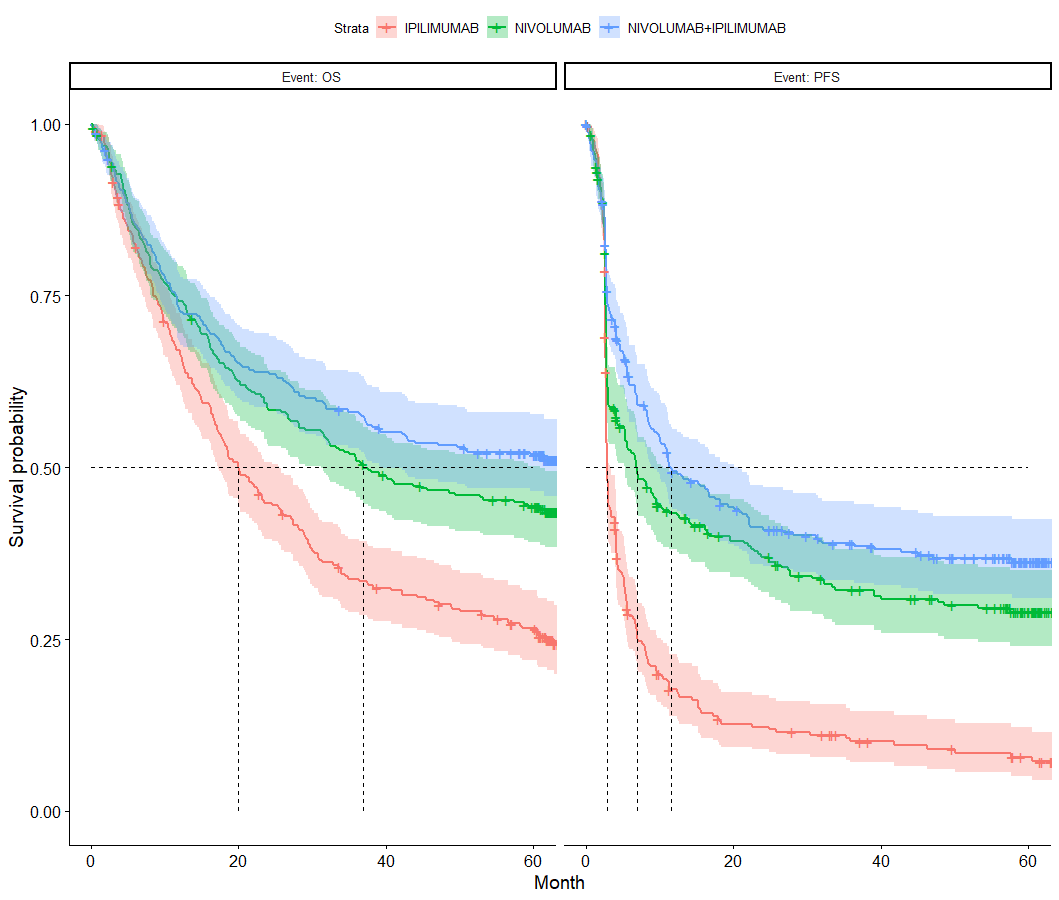
\includegraphics[width=0.6\linewidth]{S_raw_data_with_CI.png}
\caption{\label{fig:S_raw_data} Kaplan-Meier curves of OS and PFS times with 95\% CI for the Checkmate 067 study data and {\it Ipilimumab}, {\it Nivolumab} and combination treatments.
Median survival times are shown with dashed lines.}
\end{figure}

The data source for the analysis is the patient-level data from the CheckMate 067 trial [ref?].
Our dataset contains $n = 945$ subjects (8 with a missing treatment indicator, i.e. the actual treatment received).
The treatment groups are as  follows:
\begin{description}
\item[Nivolumab monotherapy] 3 mg/kg intravenous (IV) once every 2 weeks (Q2W). 313 patients were treated (203 PFS events and 175 OS events).
Median PFS and OS are 6.93 months (95\% confidence interval (CI) 5.32 - 10.41) and 36.9 months (95\% CI 31.24 - 60.9), respectively. {\it should time be in months/days?}
\item[Ipilimumab monotherapy] 3 mg/kg IV once every 3 weeks (Q3W) for a total of 4 doses.
311 patients have been treated (261 PFS events and 228 OS events). Median PFS and OS are 2.86 months (95\% CI 2.79 - 3.29) and 20.0 months (95\% CI 17.22 - 25.6), respectively.
\item[Combined nivolumab with ipilimumab] 1 mg/kg IV and 3 mg/kg IV Q3W for 4 doses followed by nivolumab 3 mg/kg IV Q2W.
313 patients were treated (182 PFS events and 151 OS events). Median PFS is 11.50 months (95\% CI 9.26 - 20.80) and median OS not reached. 
\end{description}

A full set of summary statistics can be found in the supplementary material.
%table

{\it How it compares with dataset prevalent in our field/applications? BMS?}

%
\section{Modelling framework}\label{sec:methods}
In this section, we firstly present the standard mixture cure model for a single event of interest.
Then we given our general modelling framework before focusing on the application of interest.
The model improves the typical approach used by linking multiple event-type modules using a hierarchical cure fraction.
Throughout we refer to our motivating example of jointly modelling PFS and OS.

There are two main approaches for formulating the MCM likelihood.
The first is to consider the group membership of an individual to either cured or uncured as missing data [ref].
Then the likelihood is defined in terms of the complete data and the augmented data are estimated along with the other parameters in the model, commonly using an EM algorithm.
The second approach is not to be concerned with the individual classification but rather estimate a single cure fraction for the whole sample.
This is the method used in this paper.

Assume that some patient-level time to event data are collected from a trial on $i = 1, \ldots, n$ individuals who are given treatments $j = 1, \ldots, m_i$.
Denote $T_{ij}$ to be the non-negative event times for the $i$th individual and treatment $j$.
Observe a sample of event times for some parametric distribution
\[
T \mid \bm{\theta} \sim p(t \mid \bm{\theta}).
\]
Denote $C_{ij}$ a censoring time for the $i$th individual and treatment $j$.
Then define the censoring indicator $\delta_{ij} = I(T_{ij} < C_{ij})$ and variable denoting the observed survival time $t_{ij} = \min(T_{ij}, C_{ij})$.
Either $\delta_{ij} = 1$ or $0$ denoting an event or censored observation at $t_{ij}$.
The observed data on the $i$th individual and treatment $j$ are thus
$\mathcal{O}_{ij} = (t_{ij}, \delta_{ij}, \boldsymbol{x}_{ij}),\; i = 1, \ldots, N, \; j = 1, \ldots, m_i \leq M$,
where $\boldsymbol{x}_{ij} = (x_{ij1}, \ldots, x_{ijS})$ is the individual covariate vector.
Covariates may be experimental (e.g. treatment assignment) or prognostic factors.


\subsection{The standard mixture cure model} \label{section:basic_model}

We believe the individuals to be a mixture of two distinct groups but do not observe to which group each individual belongs.
Thus, the full set of model parameters consist of two separate groups of parameters $\bm\theta = (\bm\alpha, \bm\mu)$.
The standard mixture cure model (MCM) (sometimes called a long-term survival model) has such a set-up and is the basis of the proposed model.
The MCM is a type of cure model where survival is modelled as a mixture of those who are cured and those who are not.
In the simplest case, this consists of those who will never experience the event of interest and those who remain at risk of the event.
The more general case adopted in this paper is when cured does not mean that an individual will never experience the event of interest but the chance of doing so reverts to a general or background population probability e.g. all-cause mortality.
The combined survival for a population with a cure fraction can be written as follows

\begin{equation}
\label{eqn:mcm}
S(t \mid \bm\theta, \bm{x}) = S_b(t \mid \bm\alpha, \bm{x}) [\pi(\bm{x}) + (1 - \pi(\bm{x})) S_u(t \mid \bm\mu, \bm{x})],
\end{equation}
\\
\noindent
where $S(t) = 1 - \int_0^t p(s \mid \theta) \text{d}s$ denotes survival at time $t$,
$S_b(t \mid \bm\alpha, \bm{x})$ is a function of the background mortality at time $t$ conditional on covariates $x$,
% some papers denote \pi as _uncured_ fraction
$\pi(x)$ denotes the probability of being cured conditional on covariates $x$,
and $S_u(t \mid \bm\mu, \bm{x})$ is a function of the (excess) mortality due to cancer at time $t$ conditional on covariates $x$.

The survival distributions parameters $\bm\alpha$ and $\bm\mu$ comprise of a {\it rate} $\lambda_{\alpha}$, $\lambda_{\mu}$ and a set of {\it ancillary} parameters $\phi_{\alpha}$ and $\phi_{\mu}$.
We can model the rate parameter using a generalised linear structure, e.g.
$$
g(\lambda_i) = \beta^{\lambda}_0 + \beta^{\lambda}_1 x_{age, i} \; [+ \ldots ],
$$
where $\beta^{\lambda}_0$ represents an intercept and $\beta^{\lambda}_1$ the coefficients for an individual's age $x_{age}$.
The $[+ \ldots]$ term indicates additional covariates.
All treatments are included in the same model with the following fixed effect model for the cure fraction
\begin{equation}
\label{eqn:pi_regn}
\mbox{logit}(\pi_j) = \sum_j \beta^{\pi}_j \mbox{TRT}_j \;[+ \ldots]
\end{equation}
\noindent
where $\beta^{\pi}_j$ are the regression coefficients quantifying the impact of treatment $\mbox{TRT}_j$.
The $[+ \ldots]$ term could include a frailty term in the model.
{\it Also, this would be naturally considered a "structured"/random effect in a Bayesian context - worth expanding on that?...}\\
The treatment identifier is included in the covariate vector $x$.
We will assume without loss of generalisability that all individuals have all treatments.

In many cure fraction models it is common to have $S_b(t, x) = 1$ which is reasonable in the short-term.
However, we are focused on the full life-course of an individual and so include this as a general population all-cause mortality.

%
\subsubsection{Background survival}
We used the World Health Organisation (WHO) life tables by country for the latest year available of 2016
\cite{wholifetables} to inform the background mortality $S_b(t, x)$ in (\ref{eqn:mcm}).
The baseline hazards are the expected mortality rate for each
patient at the age at which they experience the event. The mortality
data are country, age and gender adjusted, thus providing a granular account of
the different patient profiles in the trial.
The WHO reports conditional probabilities of death in 5-year intervals until age 85.
A constant annual mortality rate is reported for individuals over 85.
They assumed that no-one lives beyond 100 years.

In a Bayesian analysis there are alternative ways in which we could
model the background mortality.
For this work we shall use WHO hazard point estimates as fixed and known.
We could consider the WHO estimates to provide sufficiently accurate estimates
given the sample size and so incorporating uncertainty is not necessary.
This also forces consistency across fits.
Denote the WHO estimates for individual $i$ and treatment $j$ as
$\hat{p}_{ij}, \hat{S}_{ij}, \hat{h}_{ij}$ for the density,
survival and hazard respectively, and include these in the set of observed
data $\mathcal{O}$.

This gives
\begin{equation*}
p(t_{ij} \mid \bm\theta, \mathcal{O}_{ij}) = \hat{S}_{ij} \hat{h}_{ij}^{\delta_{ij}} \left[\pi(x_{ij}) + (1 - \pi(x_{ij})) S_u(t_{ij} \mid, \boldsymbol{x}_{ij}) h_u(t_{ij} \mid \boldsymbol{x}_{ij})^{\delta_{ij}} \right]
\end{equation*}

{\it Sharples ref re Gamma process?}


\subsection{The hierarchical mixture cure model}
{\it There may be information in one sample of event times which we can use to improve the inference from another.\\
Follow-up time can be relatively short for some of the event types and so there is missing data due to censoring.
In this case it is even more important to make use of what information we do have available from related event times, possibly with more complete data.\\
In particular, OS times are necessarily longer than PFS times so will be subject to more censoring.
The limited data can lead to considerable uncertainty.}\\

The event times are often correlated because they are for the same individual.
In our motivating example, $t_i^{OS} = t_i^{PFS} + t_i^{PPS}$ where $t_i^{PPS}$ is the duration in a post-progression state and can be $0$.\\
PFS and OS need not be for the same sample of patients.

Bivariate Normal places on the OS and PFS rates could be one option for modelling the connection\cite{Tan2018} but we will impose dependency with hyperparameters.
% Tan2018 model log HR rather than cure fraction

Figure~\ref{fig:hier_dag} shows a graphical representation of the general modelling framework described for OS and PFS.

\begin{figure}
\centering
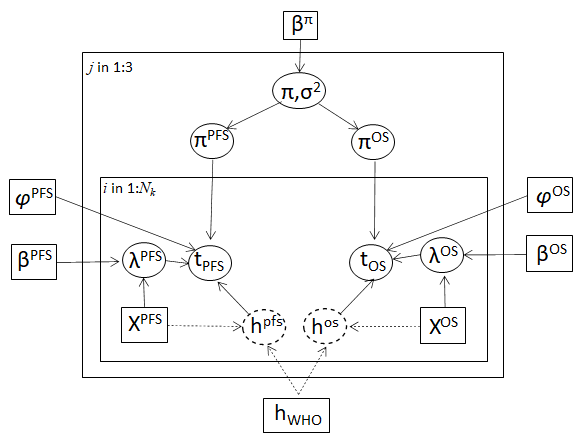
\includegraphics[width=0.6\linewidth]{DAG_with_Tx.png}
\caption{\label{fig:hier_dag} Hierarchical cure fraction DAG for PFS and OS.
Solid lines represent stochastic and dashed lines deterministic relationships, respectively.
Cured patients have fixed hazards taken from WHO life-tables.
The distribution of times for uncured patient regresses on covariates for the rate parameter and $\phi$ is the set of ancillary parameters.
Censoring has been omitted for brevity.}
\end{figure}

We extend the observed data notation and introduce index $k$ for multiple event types of interest
i.e. for the $i$th individual, $j$th treatment and $k$th event type 
$\mathcal{O} = (t_{ijk}, \delta_{ijk}, \boldsymbol{x}_{ij}), \; k = 1, \ldots, K$.
In our motivating example $K = 2$ for progression-free survival and overall survival.
The set of covariates used can be different for each $k$ and $\pi$.

The joint model is
$$
p(t \mid \boldsymbol{\beta^{\pi}}, \boldsymbol{\alpha^1}, \ldots, \boldsymbol{\alpha^K}, \boldsymbol{\mu}, \mathcal{O}) =
\prod_k p(t_k \mid \boldsymbol{\beta^{\pi}}, \boldsymbol{\alpha^{k}}, \boldsymbol{\mu}, \mathcal{O})
$$
A multilevel frailty cure fraction model for the latent variable formulation was considered by \cite{Tawiah2020}.
A related generalisation by \cite{Balogun2020} consider a single event type but multiple co-infections with different cure fractions,
similar to how we have different cure fractions for each treatment.

%
\subsubsection{Representing the cure fraction when there are multiple event types}
In this section we consider how to construct the extended model.
We consider three alternatives.

Firstly, we can model the cure fraction corresponding to each event type completely separately, assuming that they are independent.
$$
\pi_k \perp \pi_{k'}, \; k,k' = 1, \ldots, K.
%\text{logit}(\pi_k) \sim \text{N}(\mu_k, \sigma_k^2), \; k = 1, \ldots, K.
$$
Secondly, we can assume that the cure fraction is the same for all event types and so pool the samples.
In our example, PFS can be used as a proxy for OS since there are fewer missing data.
There may be no reason why the cure fraction should be different between different event types, especially if individuals are observed for long enough.
In this case
$$
\pi_k = \pi_{k'}, \; k,k' = 1, \ldots, K.
$$
Lastly, and the approach adopted in this paper, is a compromise between the first two approaches called partial-pooling.
We propose a hierarchical structure on the cure fraction assuming exchangeability between all event types $k$ for each treatment $j$ with mean value from (\ref{eqn:pi_regn}).
$$
\text{logit}(\pi_{jk}) \sim \text{N}(\pi_j, \sigma_j^2), \; k = 1, \ldots, K.  
$$


\subsubsection{Prior specification for OS, PFS model}
Where possible the choice of priors should be informed by expert opinion and prior results.
We specify vague priors on log-scale for the coefficients of the OS and PFS rates $\log(\lambda_{OS}),  \log(\lambda_{PFS})$.
Centering the ages, the baseline is a vague prior ${\beta_0^{PFS} \sim \text{N}(0, 100),}\; {\beta_0^{OS} \sim \text{N}(0, 100)}$
and for age $\beta_{age}^{PFS} \sim \text{N}(0, 100),\; \beta_{age}^{OS} \sim \text{N}(0, 100)$.
Alternatively, we could specify the cure fraction directly using a a Beta prior distribution $\pi \sim \text{Beta}(a, b)$.
The parameters can be obtained via transformation of mean and standard deviation to allow a more natural scale for elicitation.

The hierarchical cure fraction is modelled as a fixed effect linear regression with logistic link. Each treatment coefficient prior is $\beta^{\pi}_j \sim \text{N}(-0.1, 0.4)$.
This corresponds to a prior mean cure fraction of just under 0.5, and 10\% and 1\% chance of exceeding 0.6 and 0.7 respectively.  

The random effect variance on the global cure fraction is a noninformative (folded) half-Normal \cite{Gelman2006} with 
${\sigma^2 \sim \text{N}(0, 2.5)I(0,)}$, where $\text{N}(0, 2.5)I(0,)$ denotes a normal distribution truncated at mean 0.
Alternatively, a noninformative uniform prior density on standard deviation parameters $\sigma$ is expected to generally work well when $J > 5$.
For small hierarchical variance a $\text{Gamma}(2, 0.1)$ may be preferred \cite{Chung2013}.


The background is taken directly from the WHO life-tables.
However, it is believed that the patients in the trial have a worse background survival than the average individual in the general population.
Using only the complete responders in the sample, who are clinically confirmed as cured, it is possible to obtain a posterior distribution for a hazard ratio between these and a WHO estimate baseline.
This can serve as a prior in the main model in a two-step approach.
Alternatively, prior belief could be defined explicitly using expert knowledge.
This could be elicited directly for the hazard ratio or on a natural scale, such as mean life time, and transformed.


\subsubsection{Performance measures}
We evaluated the goodness of fit of the models using out-of-sample predictions estimated with the widely applicable information criterion (WAIC) and leave-one-out cross-validation (LOO) \cite{Vehtari2017}.
These have various advantages to more common AIC and DIC and are easily obtained using the posterior sample of the Stan output.\\
% The effective number of parameters is not uniquely defined because it depends on the level of the hierarchy that is in {it focus} \cite{spiegelhalter}.
The set of parameters in the hierarchical model (and their dimensions) are
$\mathbf{\beta^{\pi}}$ (3), $\mathbf{\sigma}$ (3), $\mathbf{\beta^{\lambda}_{PFS}}$ (2), $\mathbf{\beta^{\lambda}_{OS}}$ (2), $\mathbf{\phi_{OS}}$ (1), $\mathbf{\phi_{PFS}}$ (1), $\mathbf{\pi_{OS}}$ (3), $\mathbf{\pi_{PFS}}$ (3).
Depending on the number of ancillary parameters the total is 16, 17 or 18.

{\it We also calculated the 
$\Delta S$ at months $t = 10, 20, 30, ...$\\
clinical significant vs statistical significant differences.
hazard ratio?\\
median/mean survival?}\\
\\
{\it In order to investigate potential decrease in the degree of uncertainty of the estimates as a result of borrowing of information across event-types, we calculated ratios of the width of the 95\% CrIs.
Define as the ratio of the widths of the CrIs of $\pi_{os}$ and $\pi_{pfs}$ from the hierarchical model to the width of the CrIs of the separate model.}


\section{Application}\label{sec:application}

{\it BMS data and results, with various scenarios/distributions and all the plots and tables, similar to the ones already provided.}\\
We fit our model to the Checkmate 067 data set and Exponential, Weibull, Gompertz, Log-Normal, Log-Logistic to the OS and PFS event times.\\


%% journal template
% \begin{center}
% \begin{table*}[t]%
% \caption{This is sample table caption.\label{tab1}}
% \centering
% \begin{tabular*}{500pt}{@{\extracolsep\fill}lccD{.}{.}{3}c@{\extracolsep\fill}}
% \toprule
% &\multicolumn{2}{@{}c@{}}{\textbf{Spanned heading\tnote{1}}} &lticolumn{2}{@{}c@{}}{\textbf{Spanned heading\tnote{2}}} \\\cmidrule{2-3}\cmidrule{4-5}
% \textbf{col1 head} & \textbf{col2 head}  & \textbf{col3 head}  &lticolumn{1}{@{}l@{}}{\textbf{col4 head}}  & \textbf{col5 head}   \\
% \midrule
% col1 text & col2 text  & col3 text  & 12.34  & col5 text\tnote{1}   \\
% col1 text & col2 text  & col3 text  & 1.62  & col5 text\tnote{2}   \\
% col1 text & col2 text  & col3 text  & 51.809  & col5 text   \\
% \bottomrule
% \end{tabular*}
% \begin{tablenotes}%%[341pt]
% \item Source: Example for table source text.
% \item[1] Example for a first table footnote.
% \item[2] Example for a second table footnote.
% \end{tablenotes}
% \end{table*}
% \end{center}

\subsection{Results of the model performance assessment}

% \begin{landscape}
% \begin{sidewaystable}[H]
\begin{center}
\begin{table*}[t]
\caption{WAIC statistics for hierarchical and separate models, and all distributions. \label{tab:waic}}
\begin{tabular}{llrrrrrrrrrrrr}
\toprule
\multicolumn{1}{l}{} & \multicolumn{1}{l}{} & \multicolumn{6}{c}{\textbf{Hierarchical}} & \multicolumn{6}{c}{\textbf{Separate}}\\
\cmidrule{3-8}\cmidrule{5-6}\cmidrule{9-14}
\textbf{OS distn} & \textbf{PFS distn} & \textbf{ELPD\textsuperscript{$\dagger$}} & \textbf{SE} & \textbf{$p_D^{\ddagger}$} & \textbf{SE} & \textbf{WAIC} & \textbf{SE} & \textbf{ELPD} & \textbf{SE} & $p_D$ & \textbf{SE} & \textbf{WAIC} & \textbf{SE}\\
\midrule
exp & exp & -5064.70 & 80.37 & 11.13 & 0.46 & 10129.40 & 160.74 & -5066.38 & 81.40 & 10.46 & 0.43 & 10132.76 & 162.81\\
exp & gompertz & -5065.64 & 80.44 & 11.80 & 0.49 & 10131.29 & 160.88 & -5066.68 & 81.46 & 10.38 & 0.46 & 10133.37 & 162.92\\
exp & loglogistic & -4970.34 & 80.72 & 11.78 & 0.33 & 9940.68 & 161.45 & -4971.73 & 81.67 & 10.36 & 0.28 & 9943.46 & 163.34\\
exp & lognormal & -4730.47 & 92.79 & 18.04 & 0.91 & 9460.94 & 185.59 & -4732.41 & 93.18 & 18.56 & 0.99 & 9464.83 & 186.36\\
exp & weibull & -5062.99 & 81.69 & 14.63 & 0.80 & 10125.97 & 163.38 & -5064.87 & 82.86 & 14.39 & 0.86 & 10129.74 & 165.72\\
gompertz & exp & -5064.99 & 80.41 & 11.45 & 0.45 & 10129.99 & 160.82 & -5066.72 & 81.44 & 10.51 & 0.45 & 10133.43 & 162.89\\
gompertz & gompertz & -5065.61 & 80.44 & 11.66 & 0.48 & 10131.22 & 160.88 & -5066.76 & 81.49 & 10.19 & 0.44 & 10133.53 & 162.97\\
gompertz & loglogistic & -4970.42 & 80.79 & 11.68 & 0.34 & 9940.84 & 161.59 & -4972.24 & 81.70 & 10.70 & 0.28 & 9944.47 & 163.40\\
gompertz & lognormal & -4730.92 & 92.64 & 18.31 & 0.95 & 9461.84 & 185.29 & -4732.23 & 93.30 & 18.01 & 0.95 & 9464.46 & 186.61\\
gompertz & weibull & -5063.81 & 81.74 & 15.45 & 0.85 & 10127.61 & 163.48 & -5064.46 & 82.92 & 13.50 & 0.78 & 10128.91 & 165.83\\
loglogistic & exp & -5059.86 & 80.47 & 11.29 & 0.42 & 10119.73 & 160.93 & -5062.51 & 81.89 & 10.79 & 0.40 & 10125.02 & 163.78\\
loglogistic & gompertz & -5060.37 & 80.40 & 11.64 & 0.45 & 10120.74 & 160.80 & -5062.64 & 82.01 & 10.26 & 0.41 & 10125.27 & 164.02\\
loglogistic & loglogistic & -4966.22 & 80.75 & 12.77 & 0.35 & 9932.44 & 161.50 & -4968.45 & 82.36 & 11.63 & 0.28 & 9936.89 & 164.72\\
loglogistic & lognormal & -4726.57 & 93.17 & 19.43 & 0.91 & 9453.13 & 186.34 & -4728.25 & 94.20 & 18.18 & 0.92 & 9456.51 & 188.40\\
loglogistic & weibull & -5058.17 & 81.84 & 14.80 & 0.74 & 10116.33 & 163.67 & -5060.18 & 83.31 & 13.79 & 0.69 & 10120.37 & 166.62\\
lognormal & exp & -4972.55 & 84.58 & 16.35 & 0.61 & 9945.09 & 169.15 & -4973.43 & 85.26 & 14.63 & 0.55 & 9946.86 & 170.53\\
lognormal & gompertz & -4973.16 & 84.69 & 16.50 & 0.56 & 9946.32 & 169.38 & -4973.48 & 85.22 & 14.31 & 0.51 & 9946.96 & 170.44\\
lognormal & loglogistic & -4877.87 & 85.79 & 16.53 & 0.50 & 9755.74 & 171.59 & -4879.07 & 86.55 & 15.07 & 0.44 & 9758.14 & 173.09\\
lognormal & lognormal & -4638.85 & 100.27 & 23.58 & 1.00 & 9277.71 & 200.55 & -4638.43 & 100.40 & 21.30 & 0.96 & 9276.85 & 200.80\\
lognormal & weibull & -4970.22 & 86.17 & 19.01 & 0.89 & 9940.44 & 172.34 & -4972.48 & 87.07 & 19.54 & 0.91 & 9944.95 & 174.13\\
weibull & exp & -5063.26 & 80.70 & 11.93 & 0.46 & 10126.53 & 161.40 & -5064.74 & 81.52 & 11.11 & 0.45 & 10129.48 & 163.04\\
weibull & gompertz & -5064.37 & 80.64 & 12.67 & 0.52 & 10128.73 & 161.28 & -5065.16 & 81.59 & 11.16 & 0.44 & 10130.32 & 163.18\\
weibull & lognormal & -4729.78 & 93.18 & 19.54 & 0.97 & 9459.56 & 186.36 & -4730.93 & 93.78 & 19.04 & 0.96 & 9461.85 & 187.56\\
weibull & weibull & -5061.91 & 82.05 & 15.77 & 0.85 & 10123.81 & 164.11 & -5063.20 & 83.09 & 14.87 & 0.83 & 10126.41 & 166.17\\
\bottomrule
\end{tabular}
\begin{tablenotes}%%[341pt]
\textsuperscript{$\dagger$}ELPD: Expected log pointwise predictive density;
\textsuperscript{$\ddagger$}$p_D$: Effective number of parameters
\end{tablenotes}
\end{table*}
\end{center}
% \end{sidewaystable}
% \end{landscape}

% \begin{landscape}
% \begin{sidewaysfigure}[H]
\begin{figure}
\centering
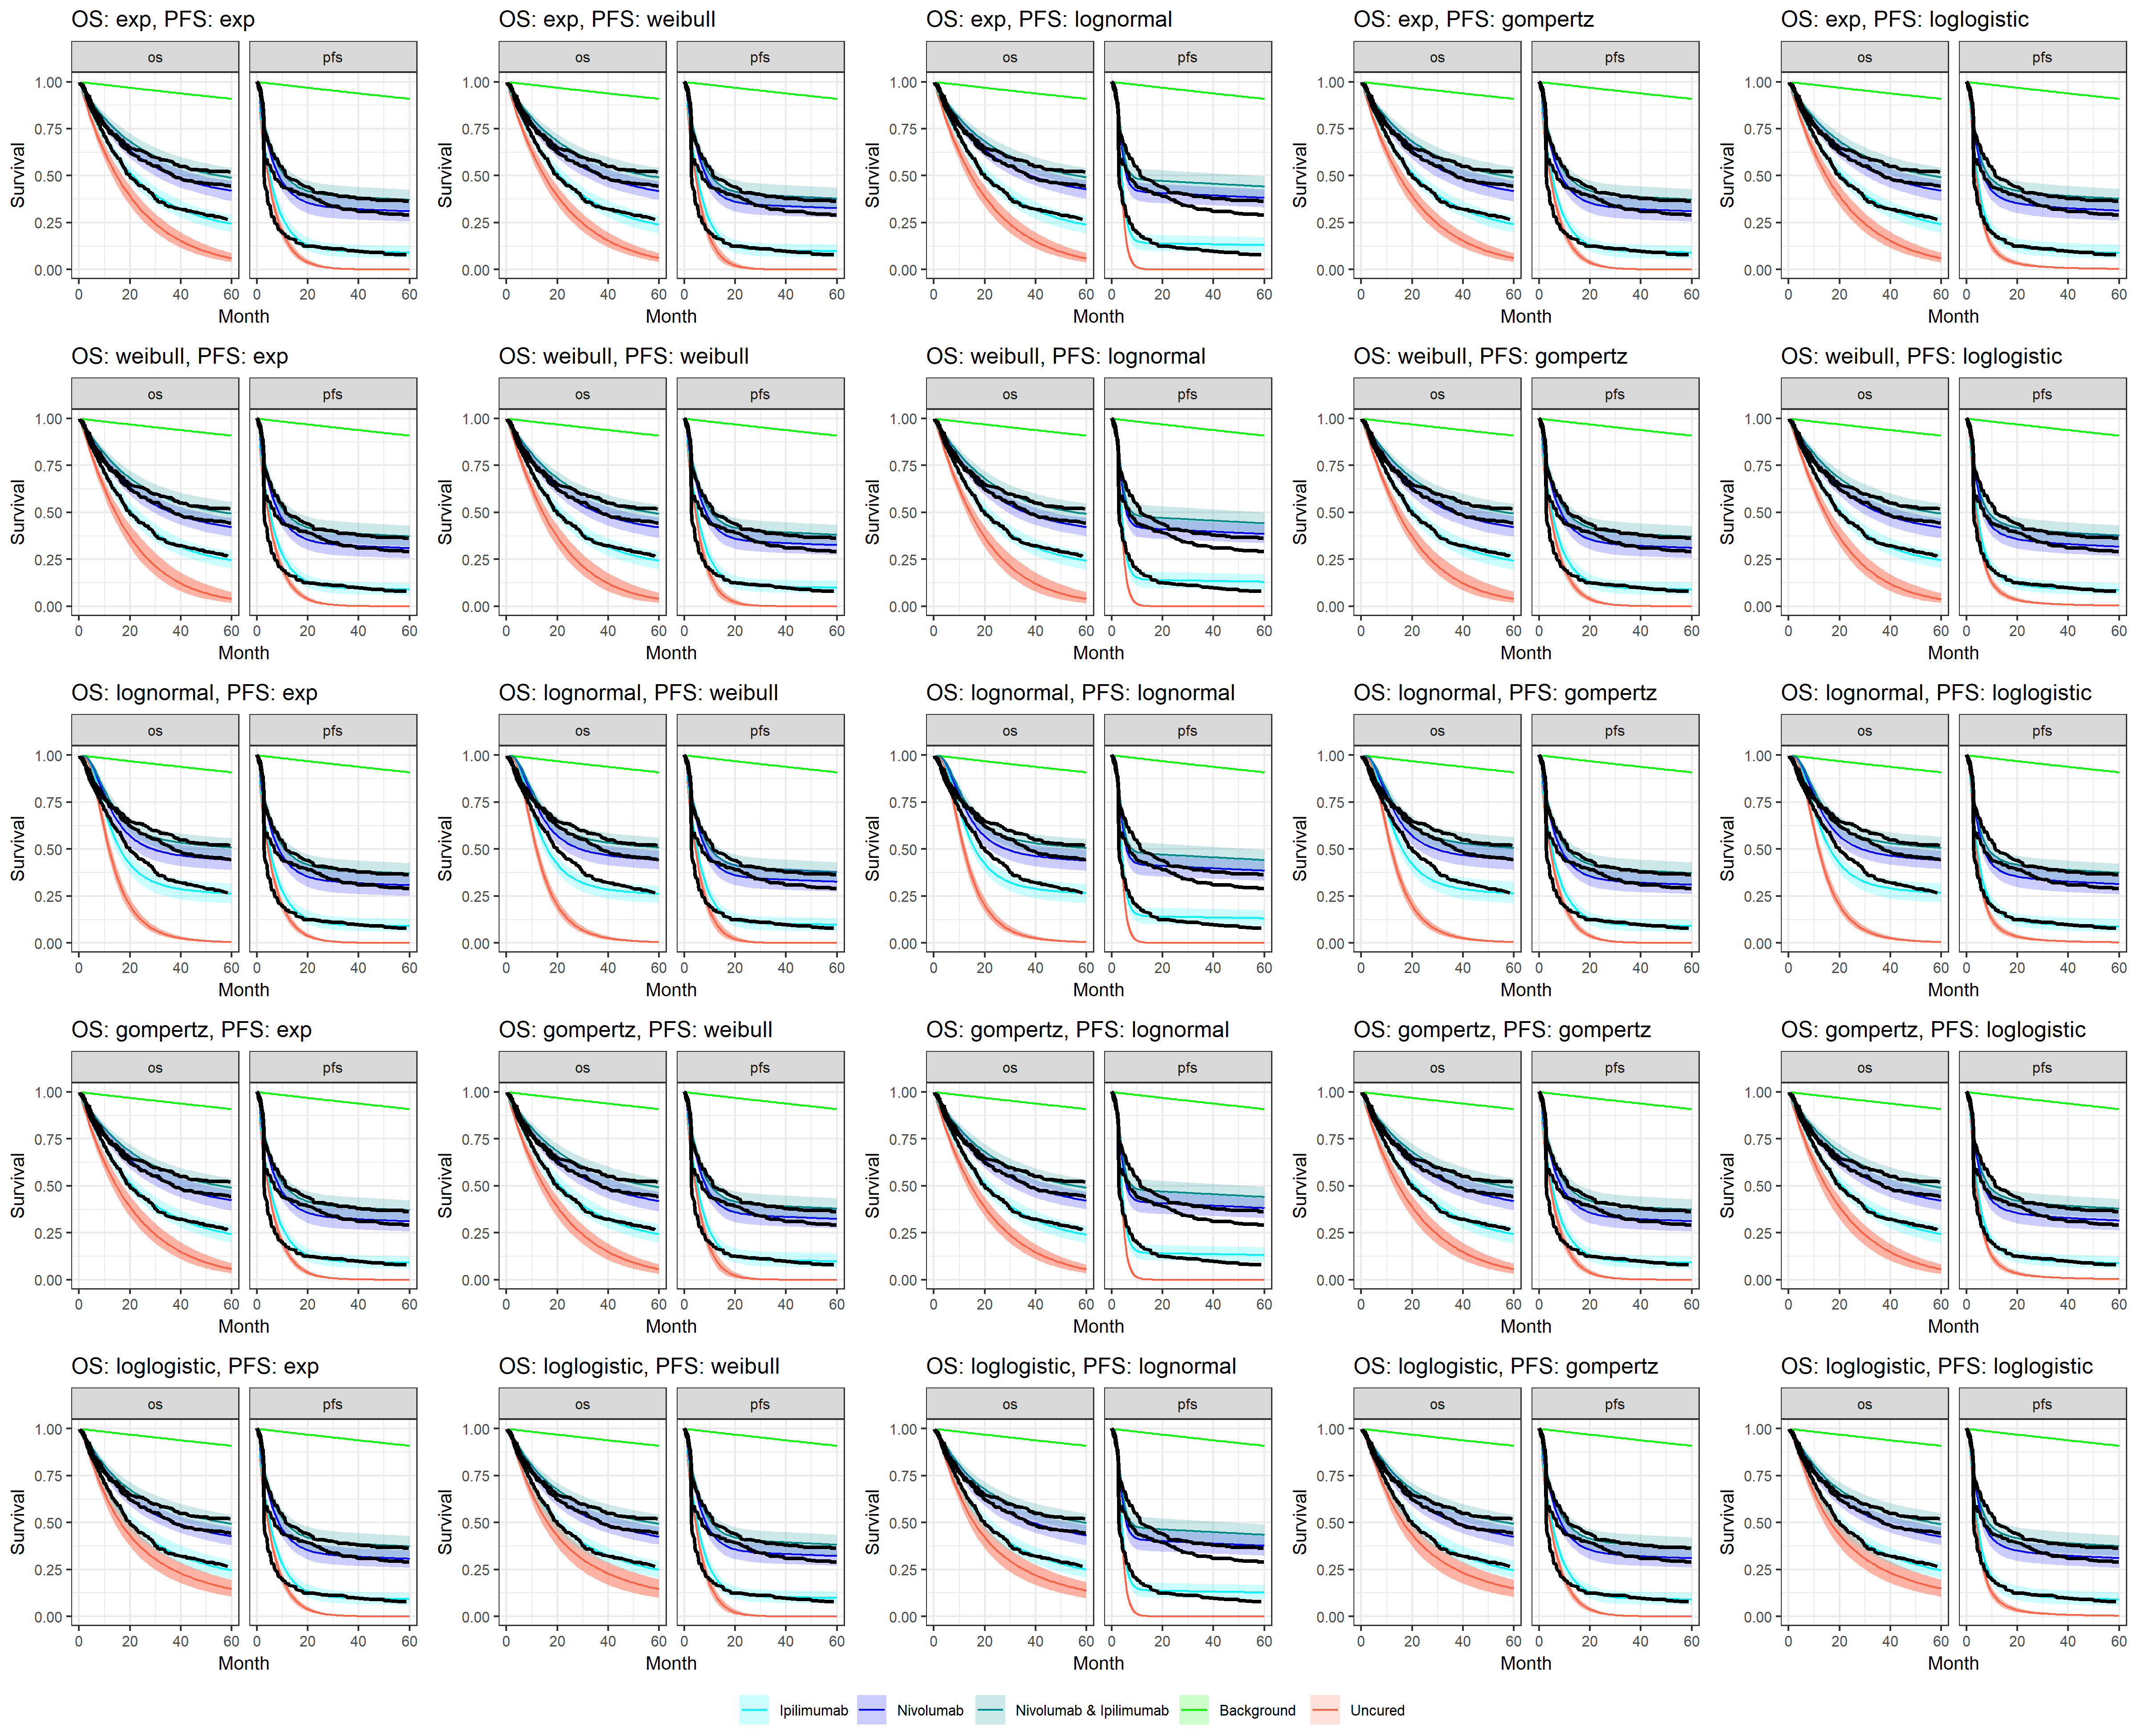
\includegraphics[width=0.9\linewidth]{plot_S_grid_cf_hier.png}
\caption{\label{fig:S_grid_cf_hier} Hierarchical model posterior survival curves for exponential, weibull, gompertz, log-logistic and log-Normal uncured fraction for OS and PFS events and {\it ipilimumab}, {\it nivolumab} and combination treatments. The black lines show the Kaplan-Meier curves.}
\end{figure}
% \end{sidewaysfigure}
% \end{landscape}

% \begin{sidewaysfigure}[H]
% 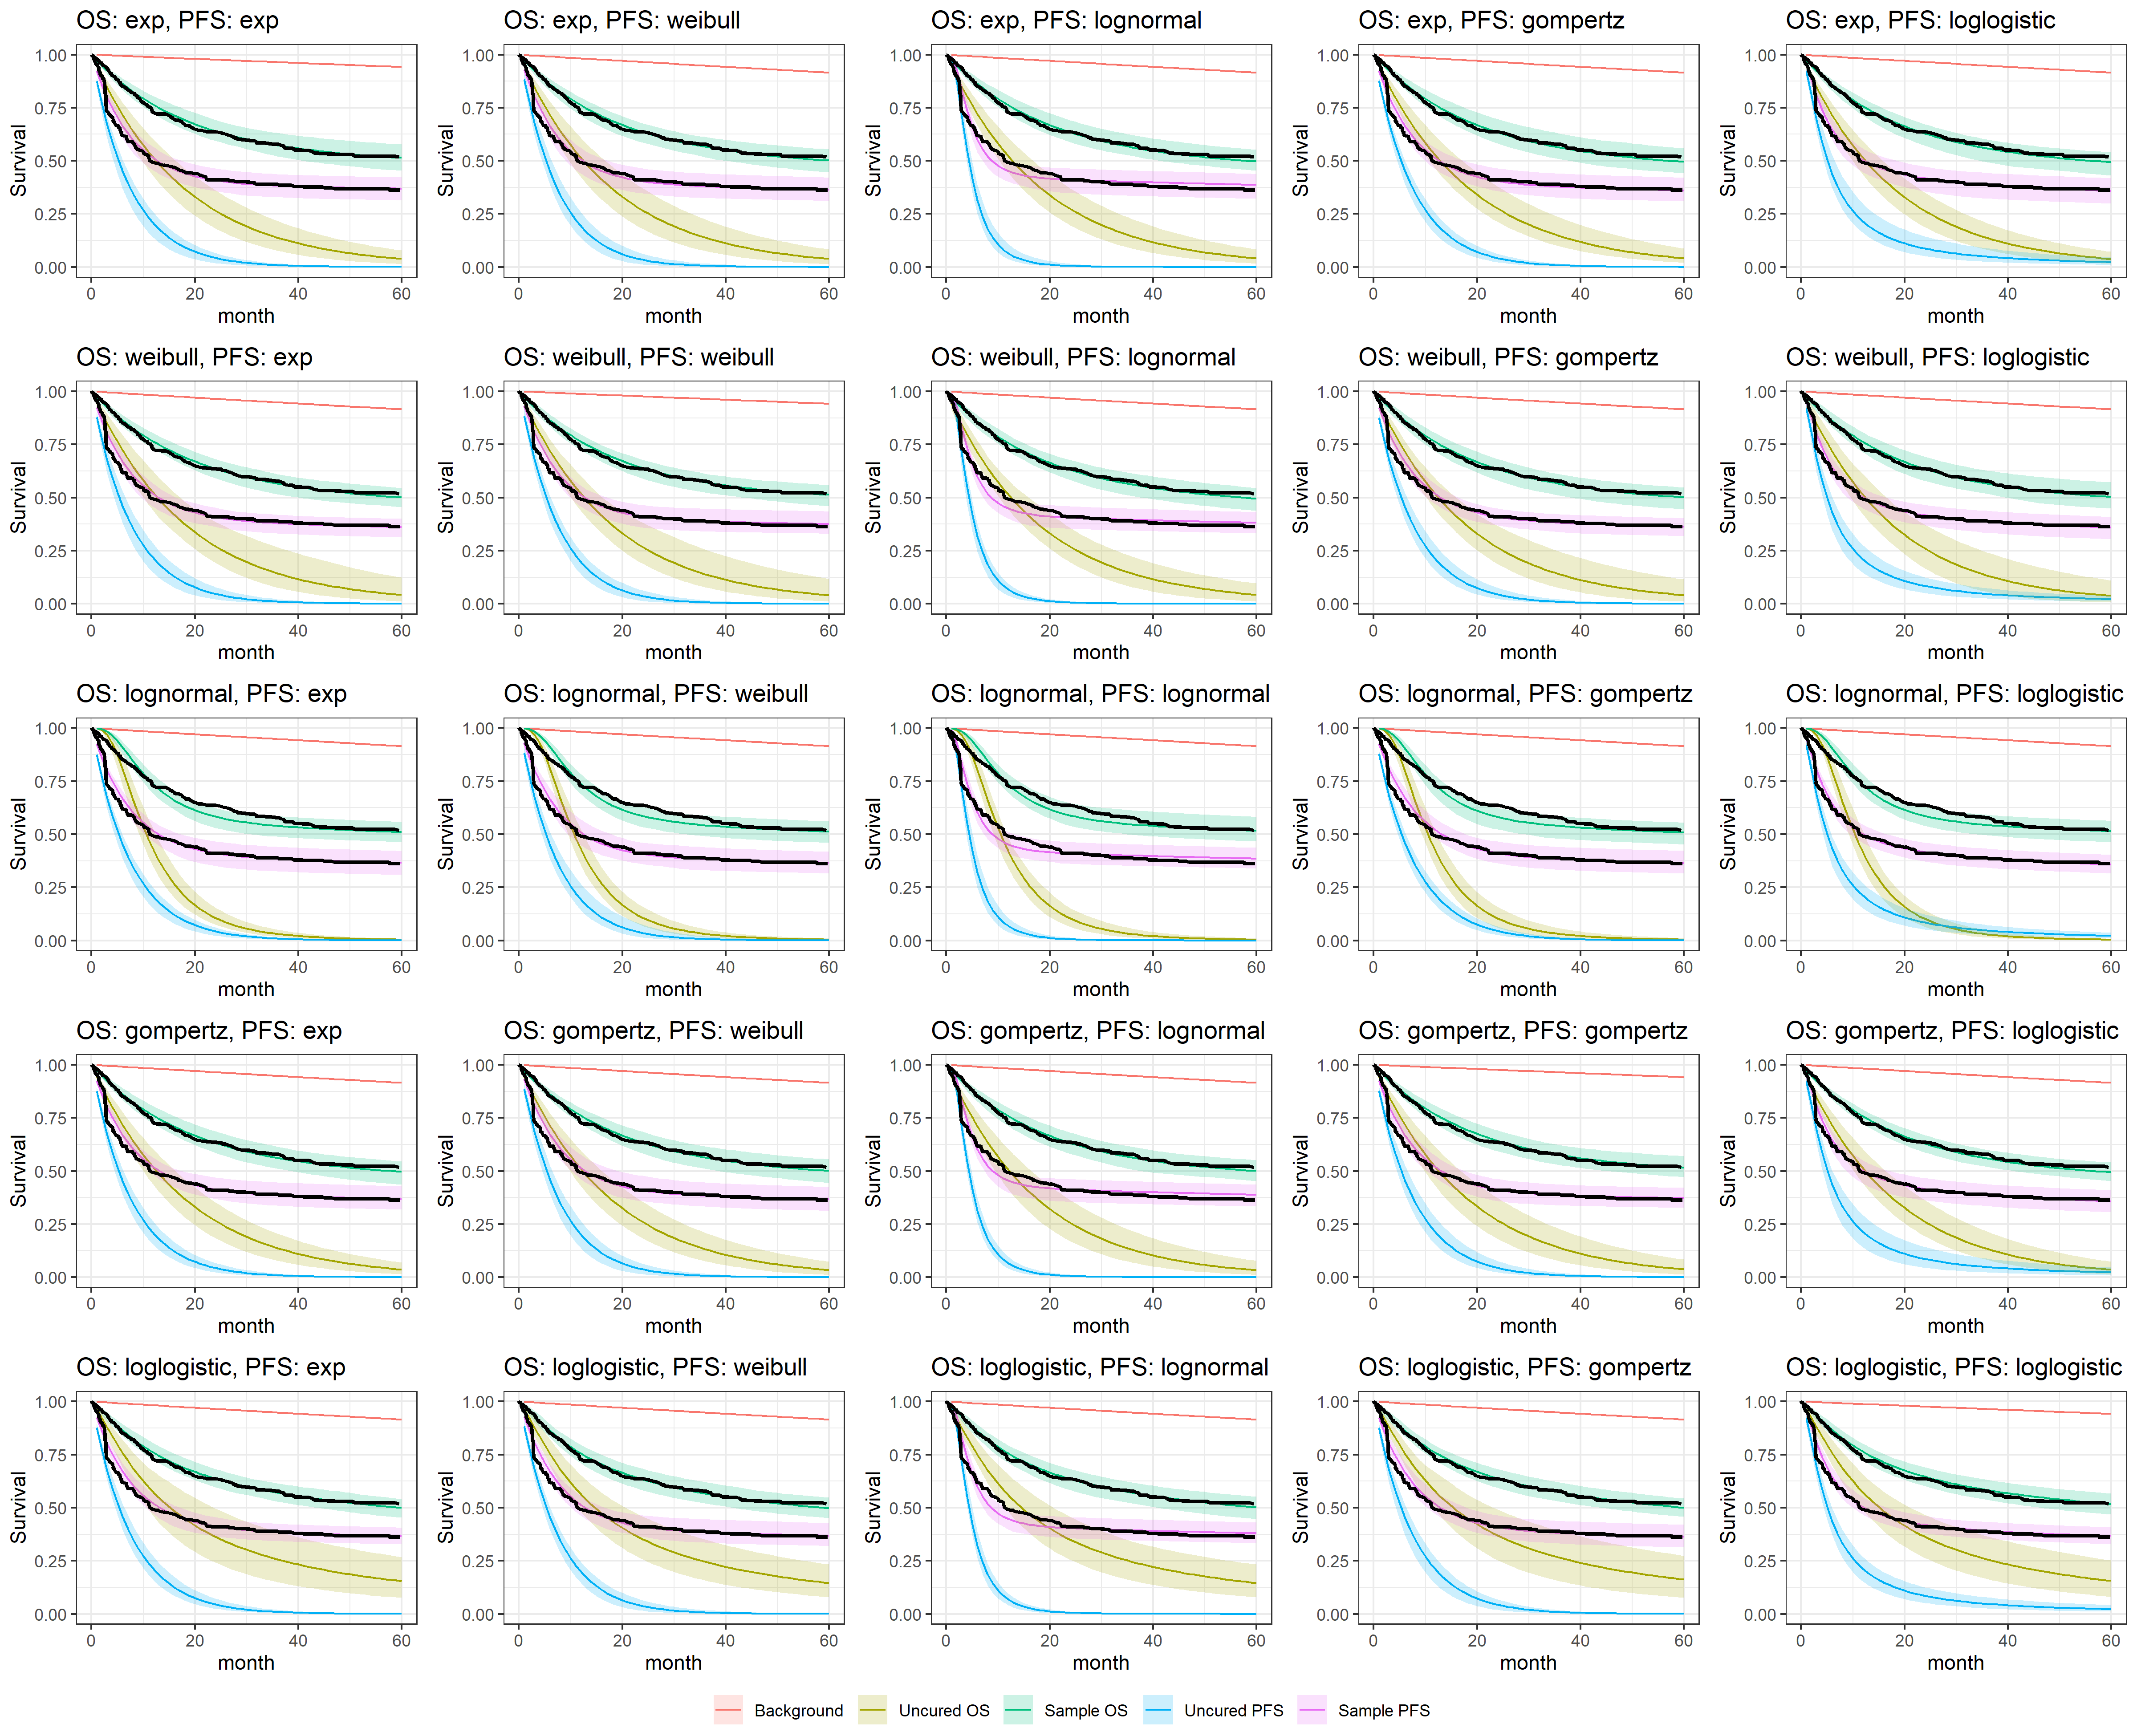
\includegraphics[width=0.9\linewidth]{plot_S_grid.png}
% \caption{\label{fig:S_grid_ipi_nivo} Hierarchical model posterior survival curves for exponential, weibull, gompertz, log-logistic and log-Normal uncured fraction for OS and PFS events and {\it nivolumab} and {\it ipilimumab} combination treatment. The black lines show the Kaplan-Meier curves.}
% \end{sidewaysfigure}

% \begin{sidewaysfigure}[H]
% 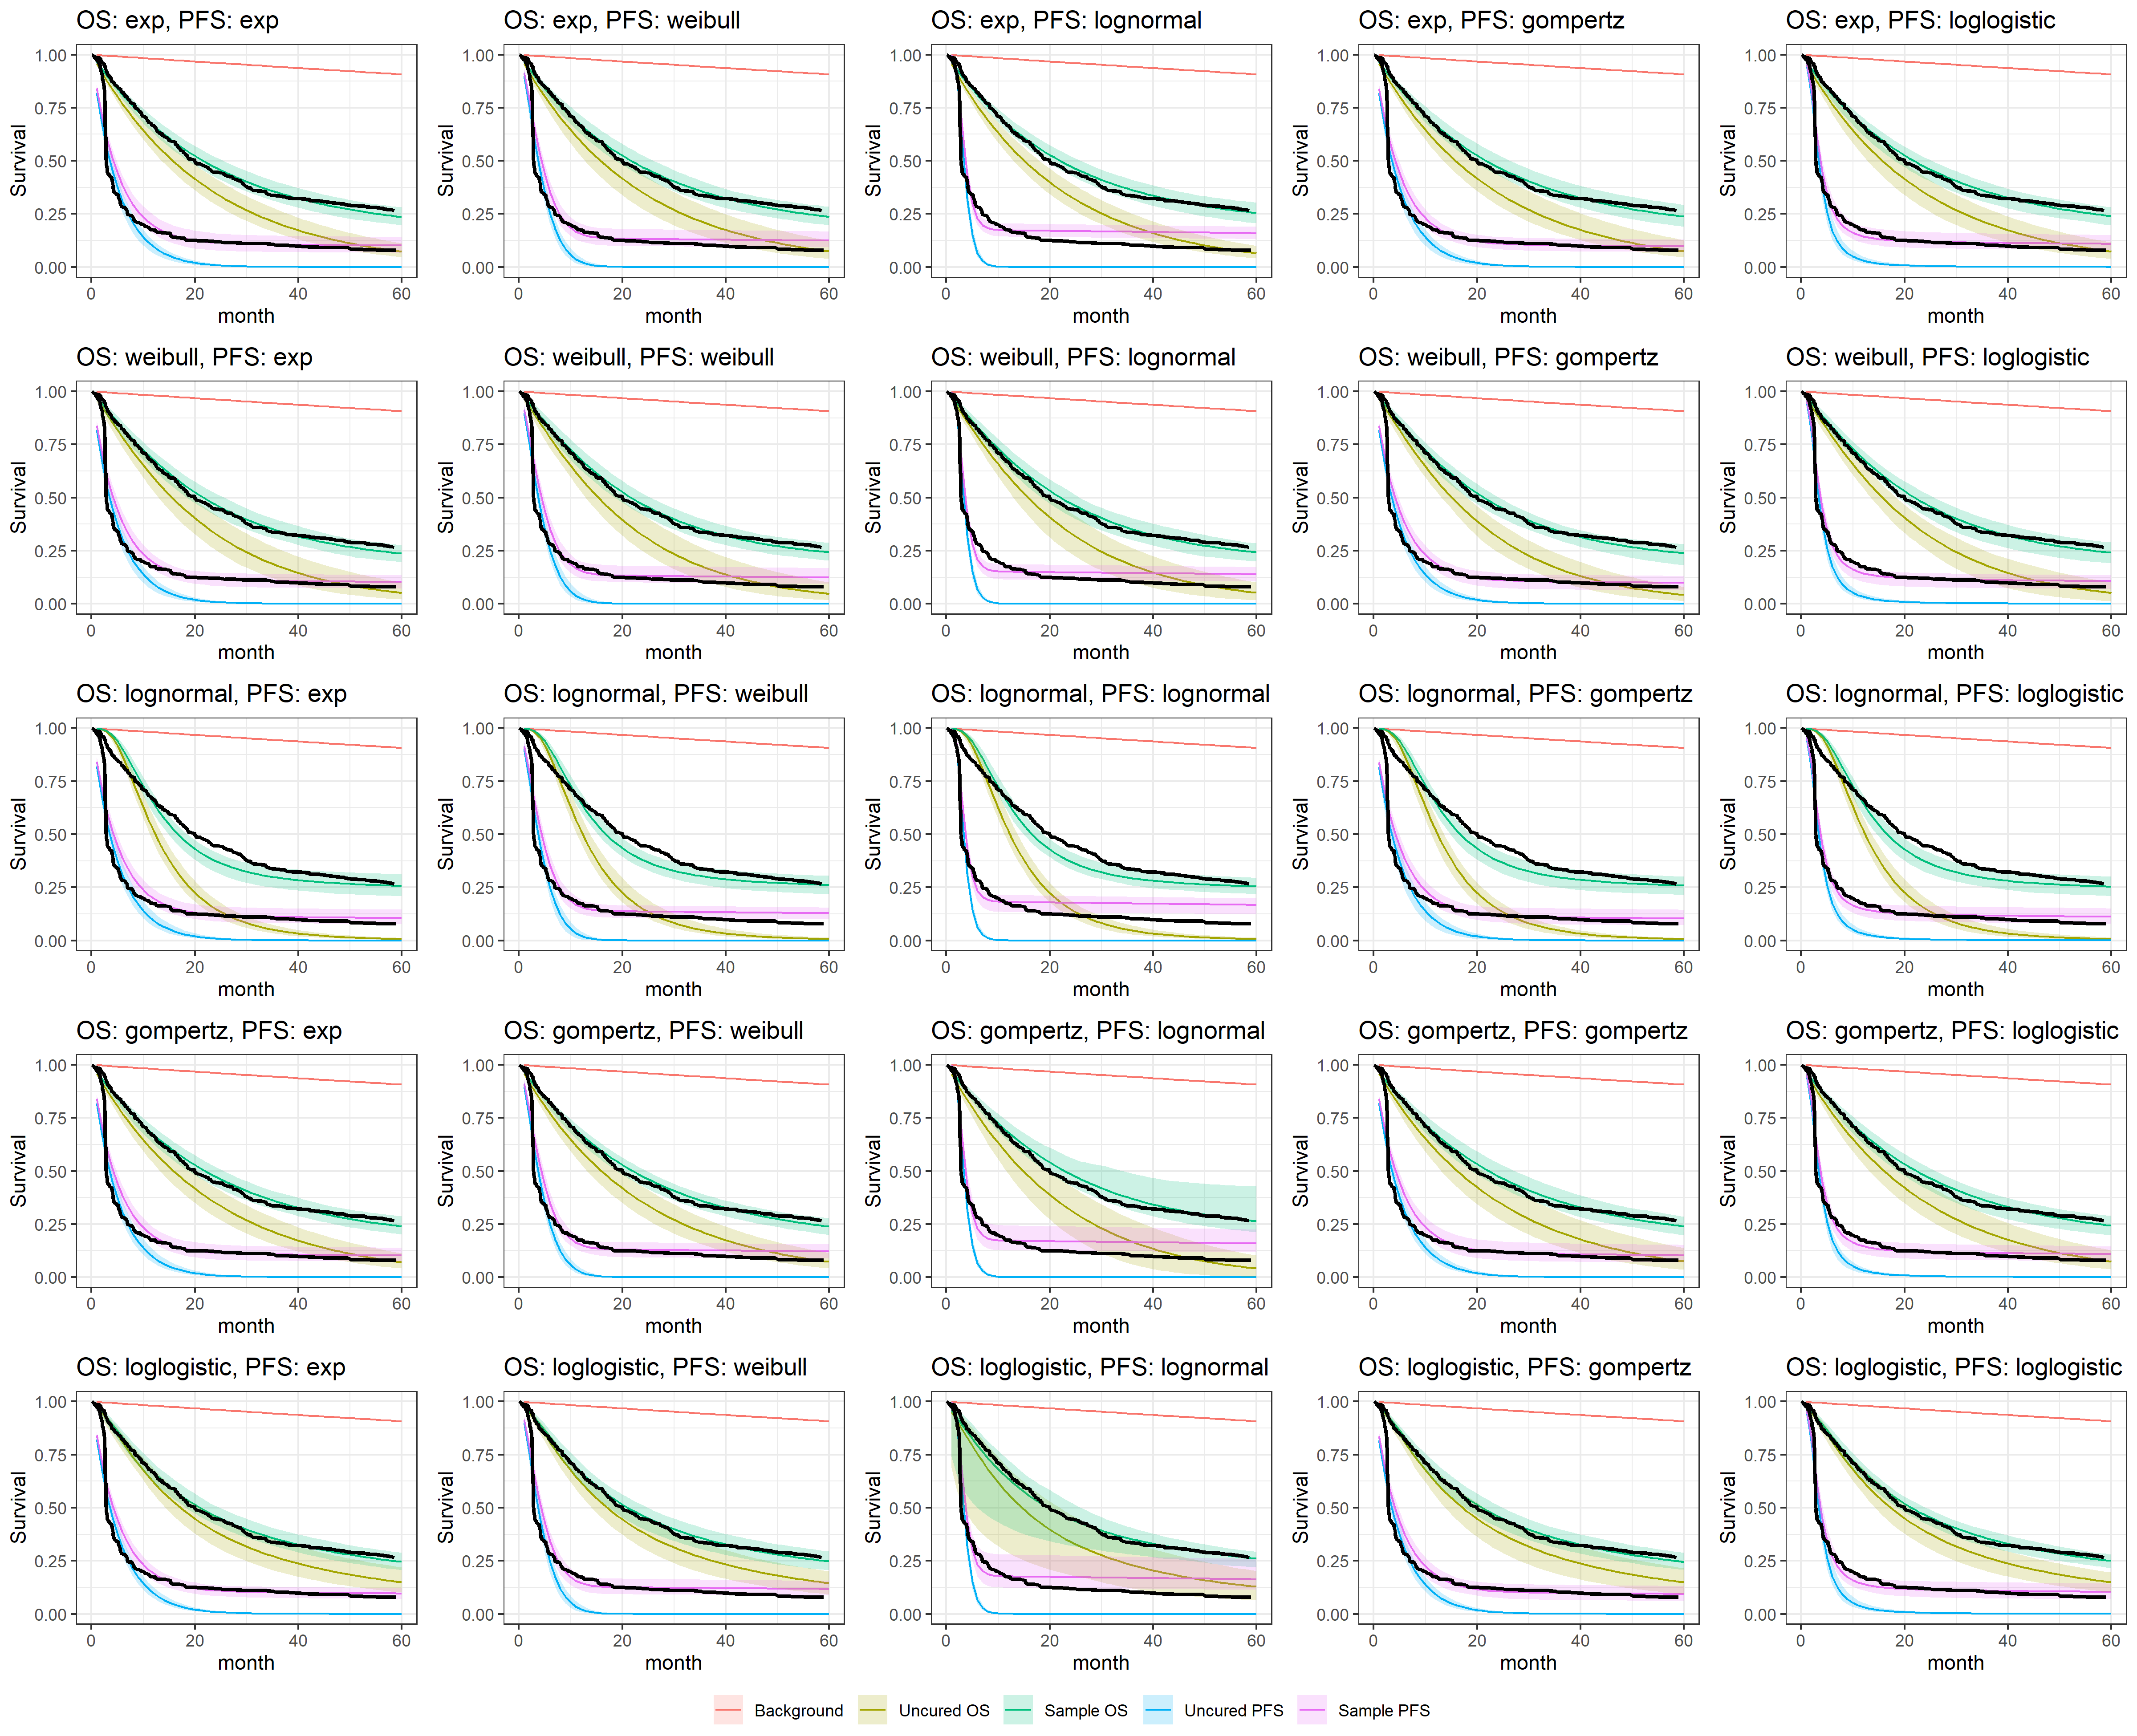
\includegraphics[width=0.9\linewidth]{plot_S_grid_IPILIMUMAB.png}
% \caption{\label{fig:S_grid_ipi} Hierarchical model posterior survival curves for exponential, weibull, gompertz, log-logistic and log-Normal uncured fraction for OS and PFS events and {\it ipilimumab} treatment. The black lines show the Kaplan-Meier curves.}
% \end{sidewaysfigure}

% \begin{sidewaysfigure}[H]
% 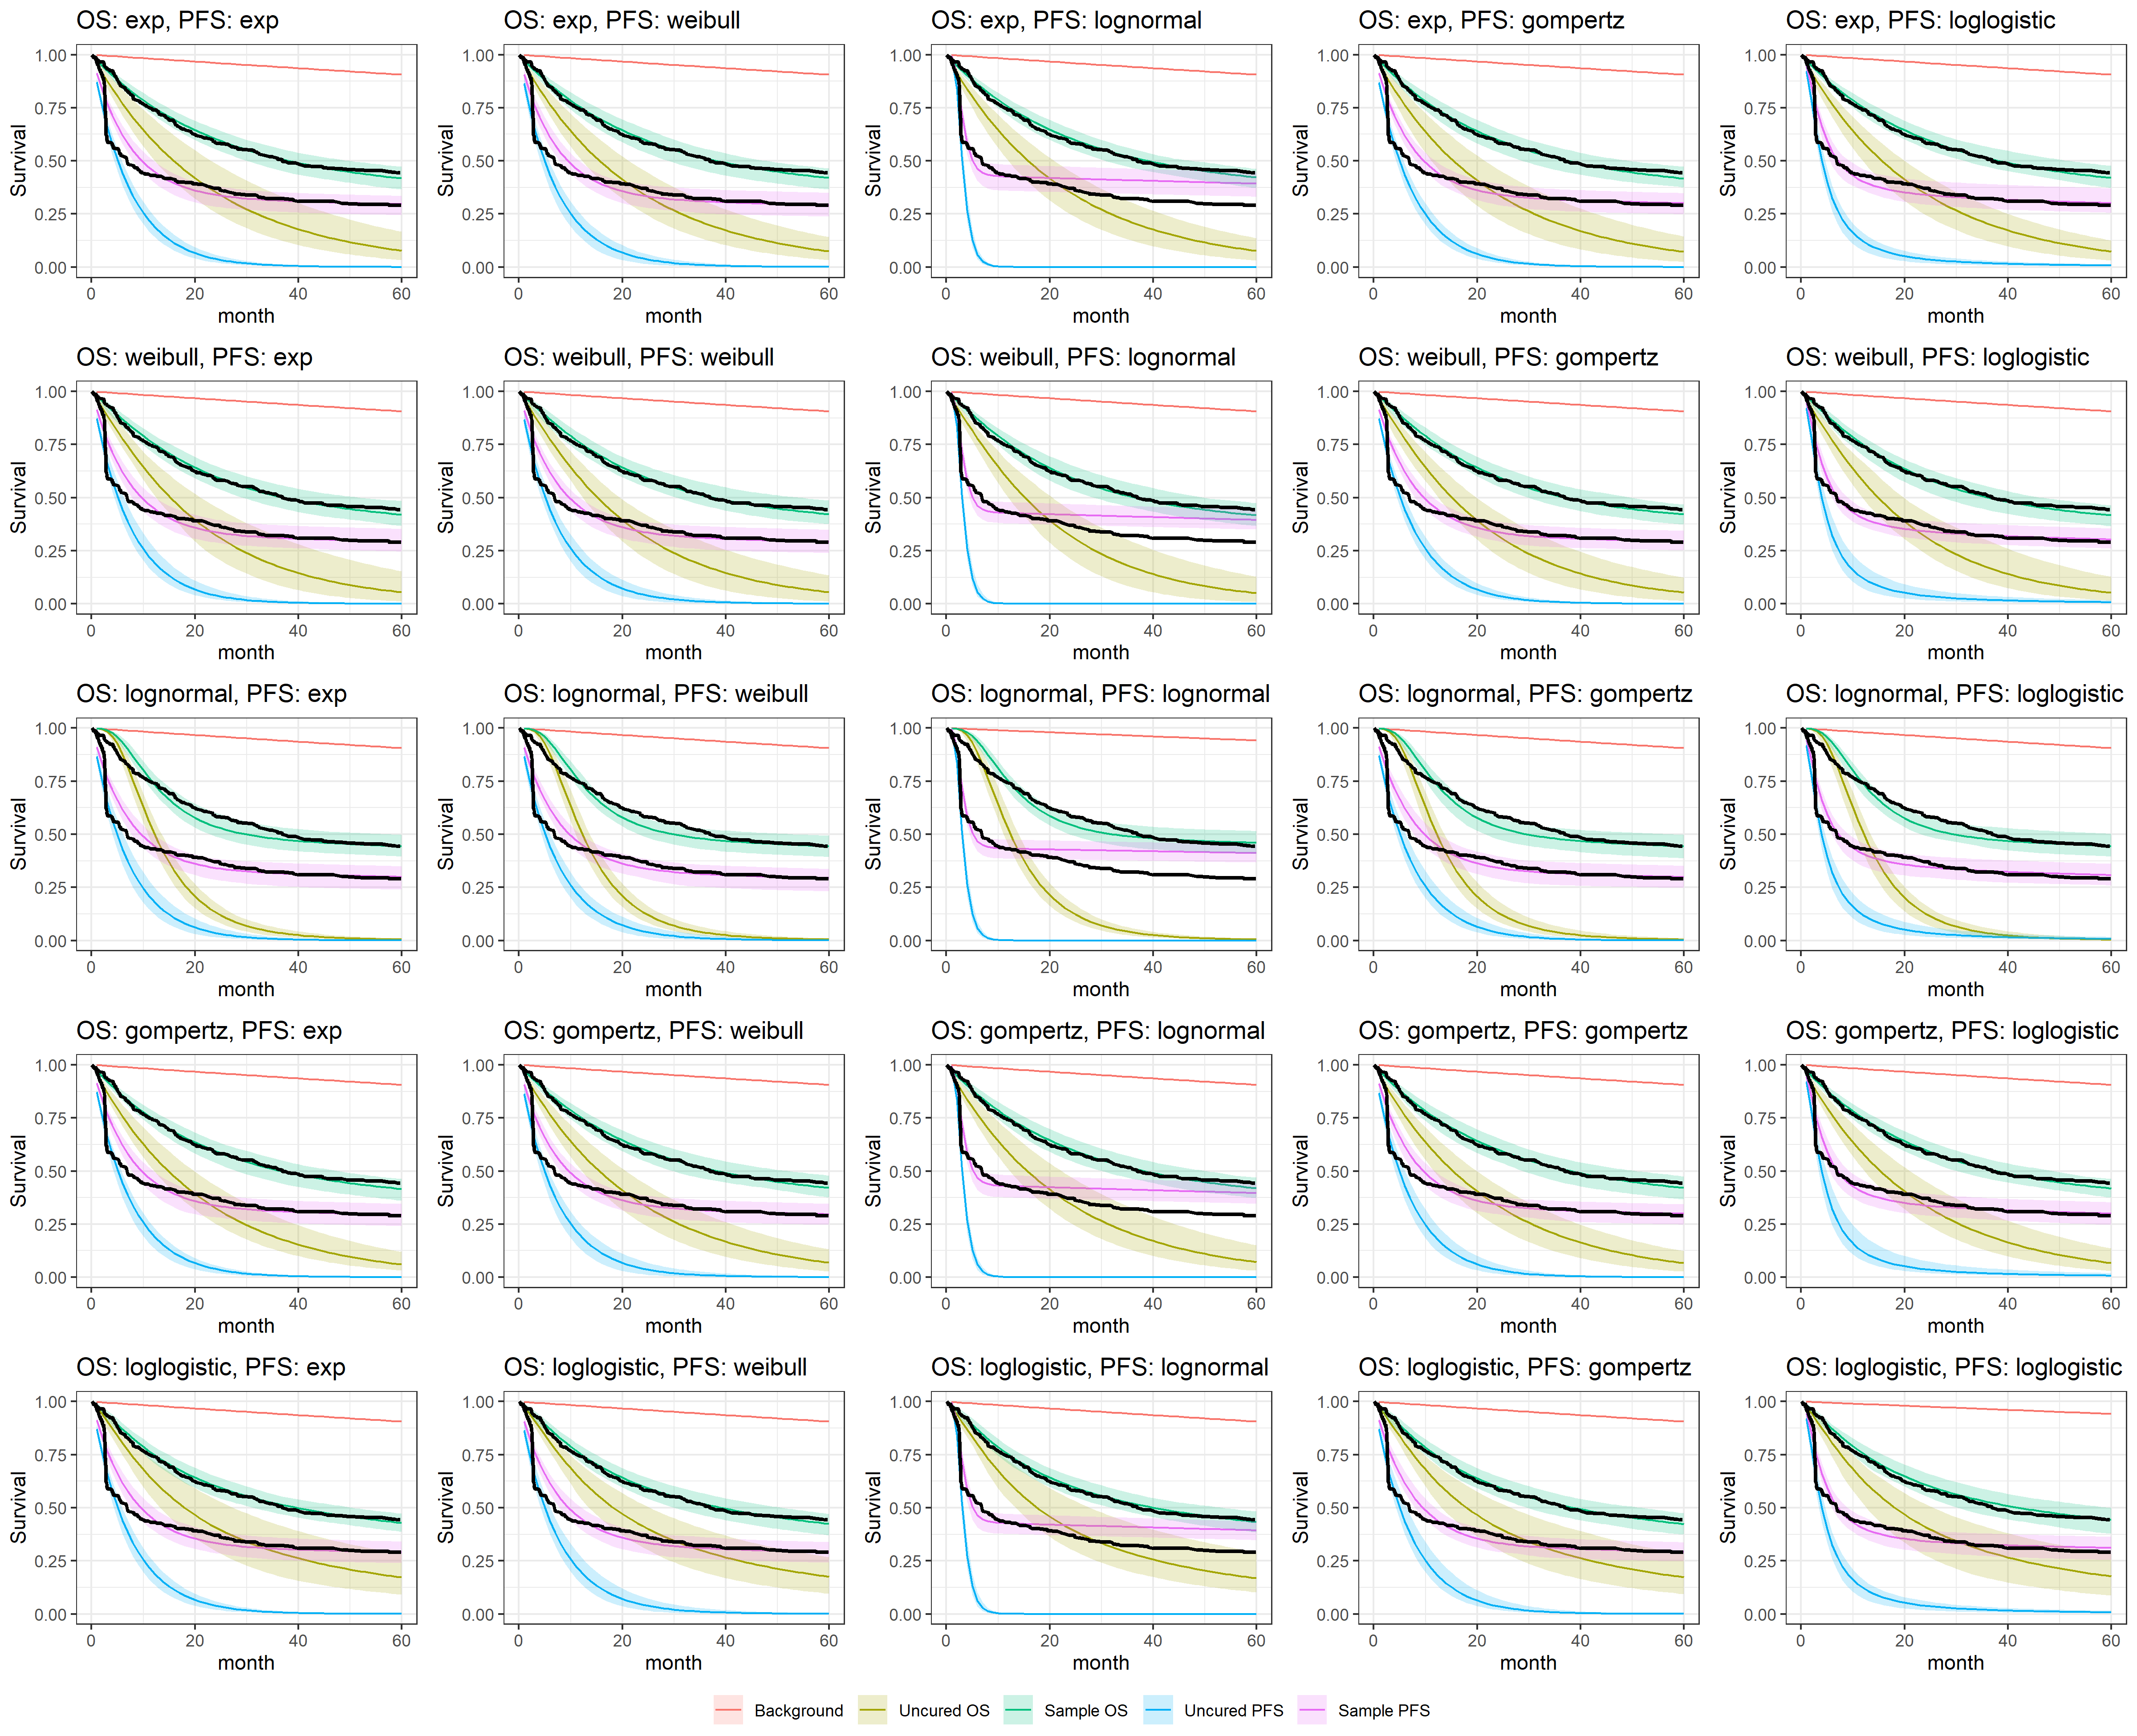
\includegraphics[width=0.9\linewidth]{plot_S_grid_NIVOLUMAB.png}
% \caption{\label{fig:S_grid_nivo} Hierarchical model posterior survival curves for exponential, weibull, gompertz, log-logistic and log-Normal uncured fraction for OS and PFS events and {\it nivolumab} treatment. The black lines show the Kaplan-Meier curves.}
% \end{sidewaysfigure}

% \begin{landscape}
% \begin{sidewaysfigure}[H]
\begin{figure}
\centering
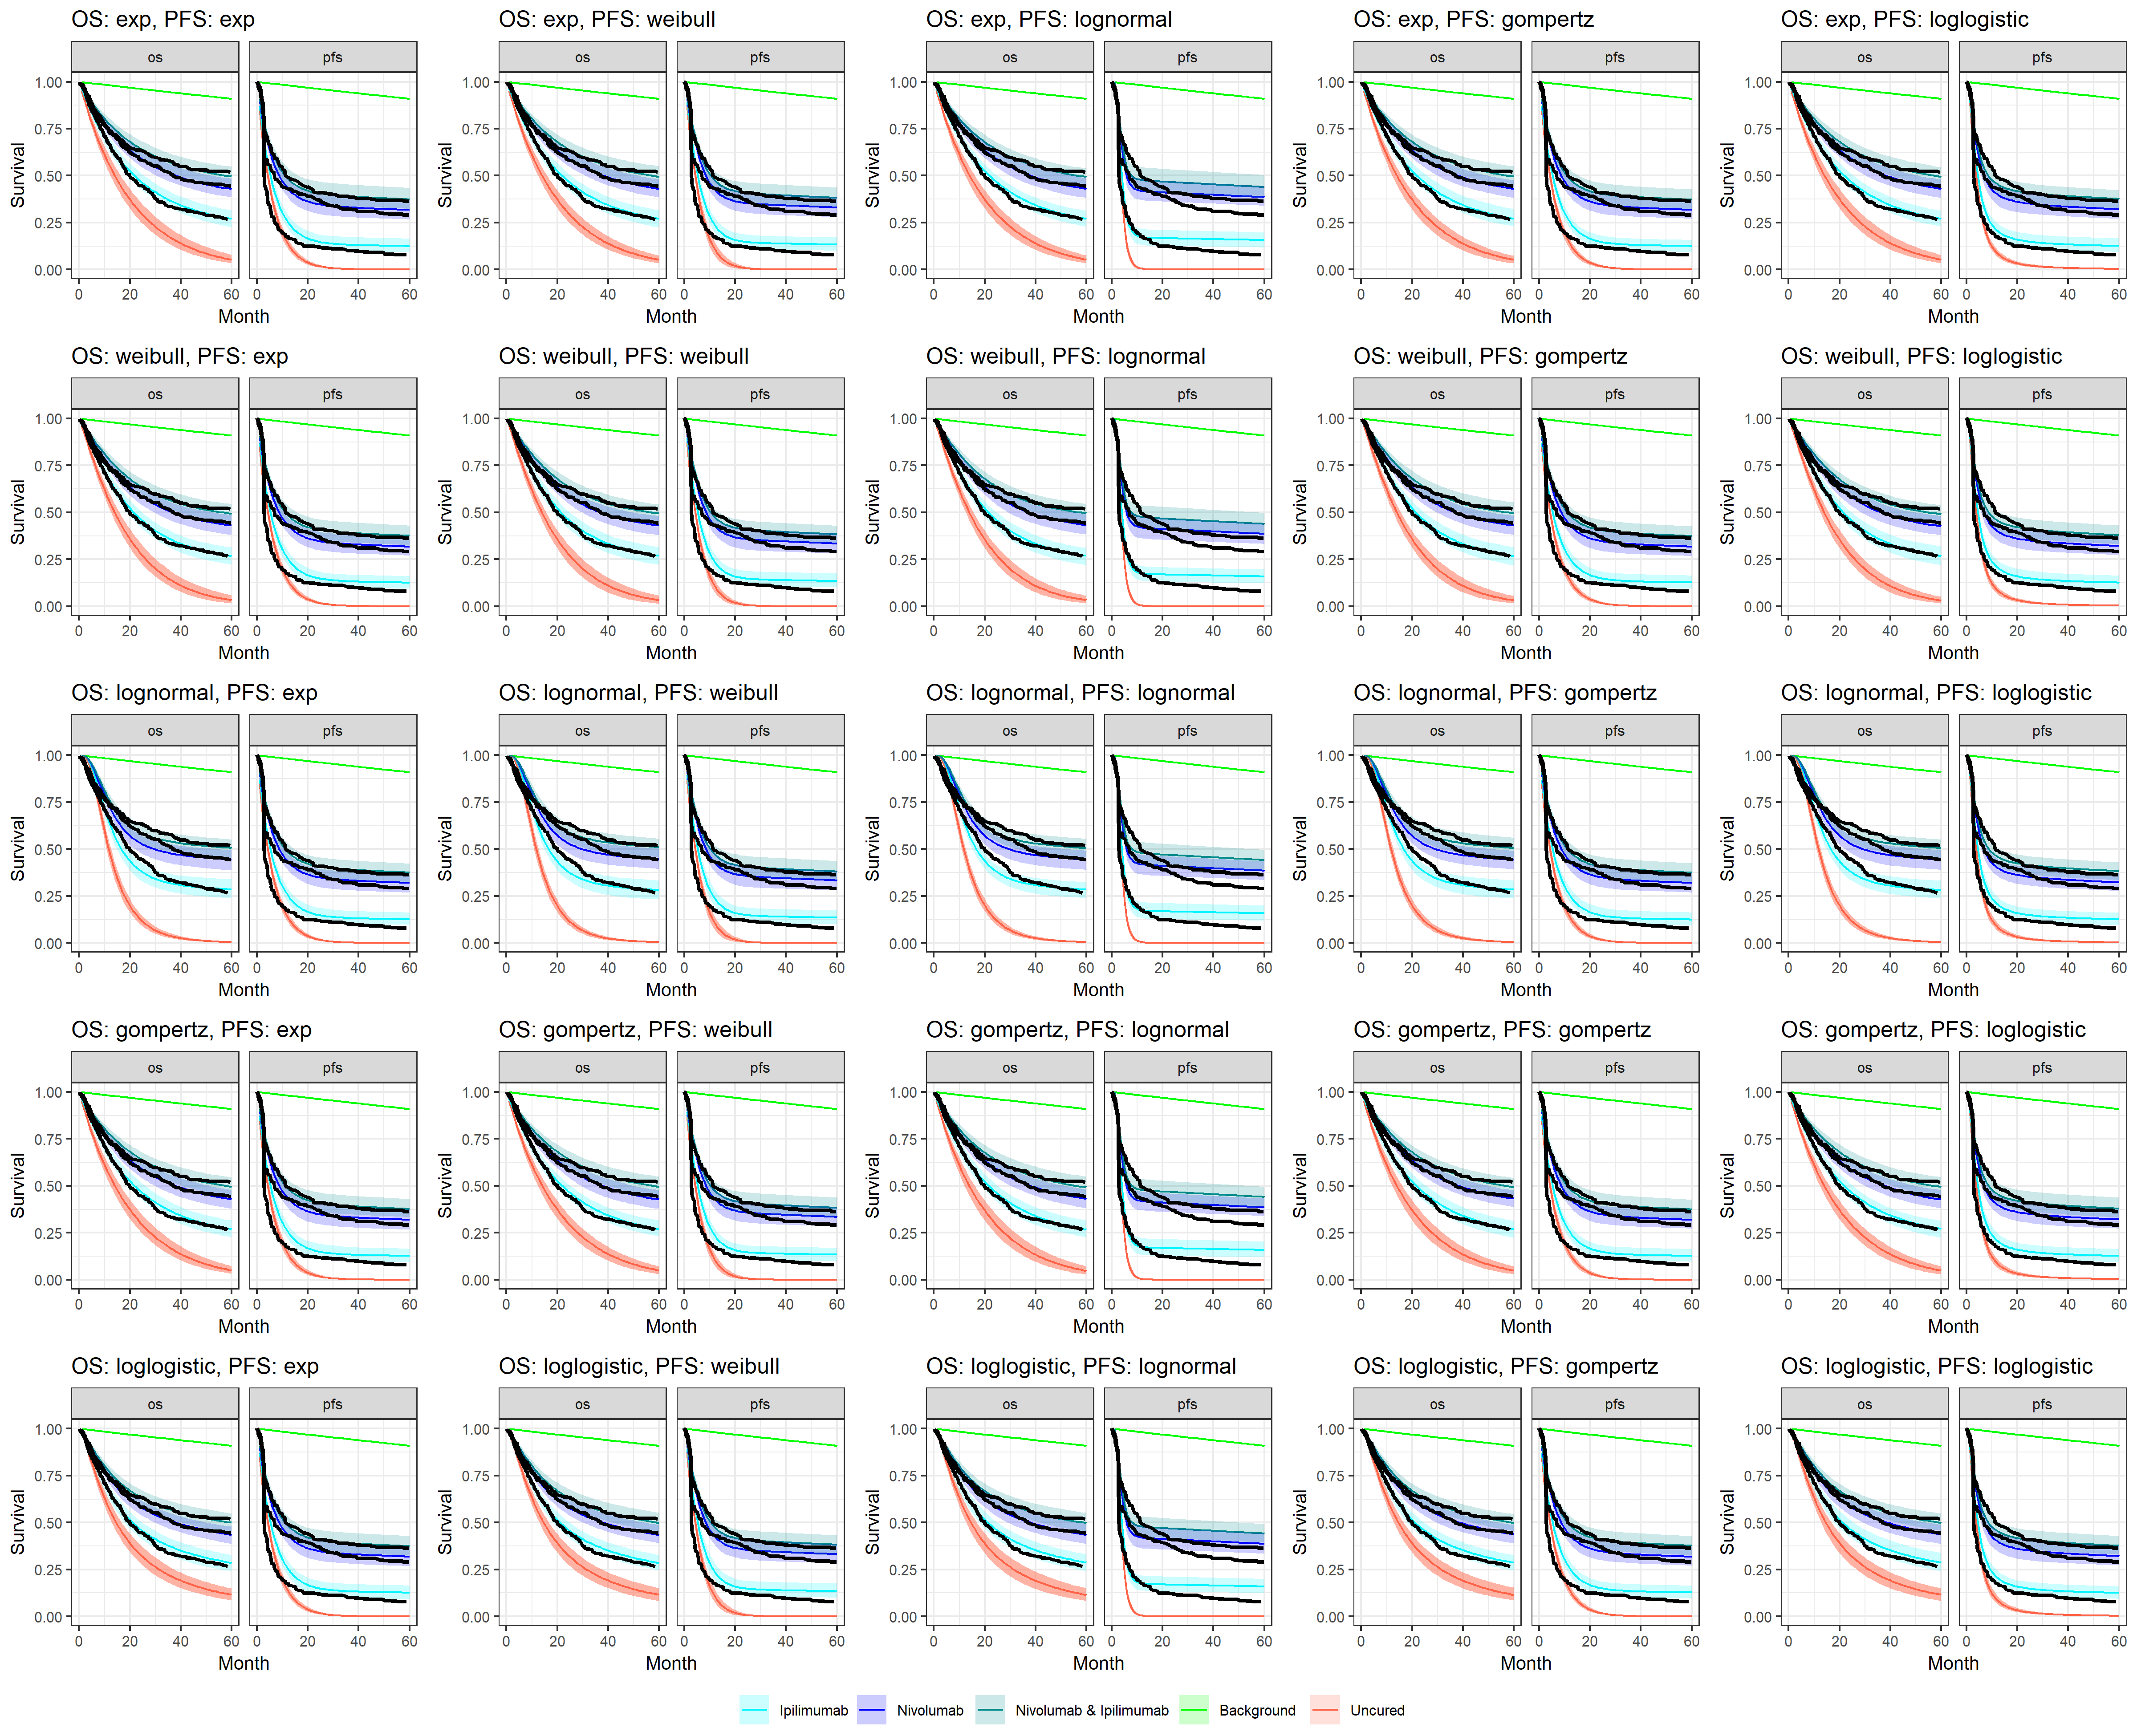
\includegraphics[width=0.9\linewidth]{plot_S_grid_cf_separate.png}
\caption{\label{fig:S_grid_separate} Separate model posterior survival curves for exponential, weibull, gompertz, log-logistic and log-Normal uncured fraction for OS and PFS events {\it ipilimumab}, {\it nivolumab} and combination treatments. The black lines show the Kaplan-Meier curves.}
\end{figure}
% \end{sidewaysfigure}
% \end{landscape}

% \begin{figure}[H]
% \centering
% 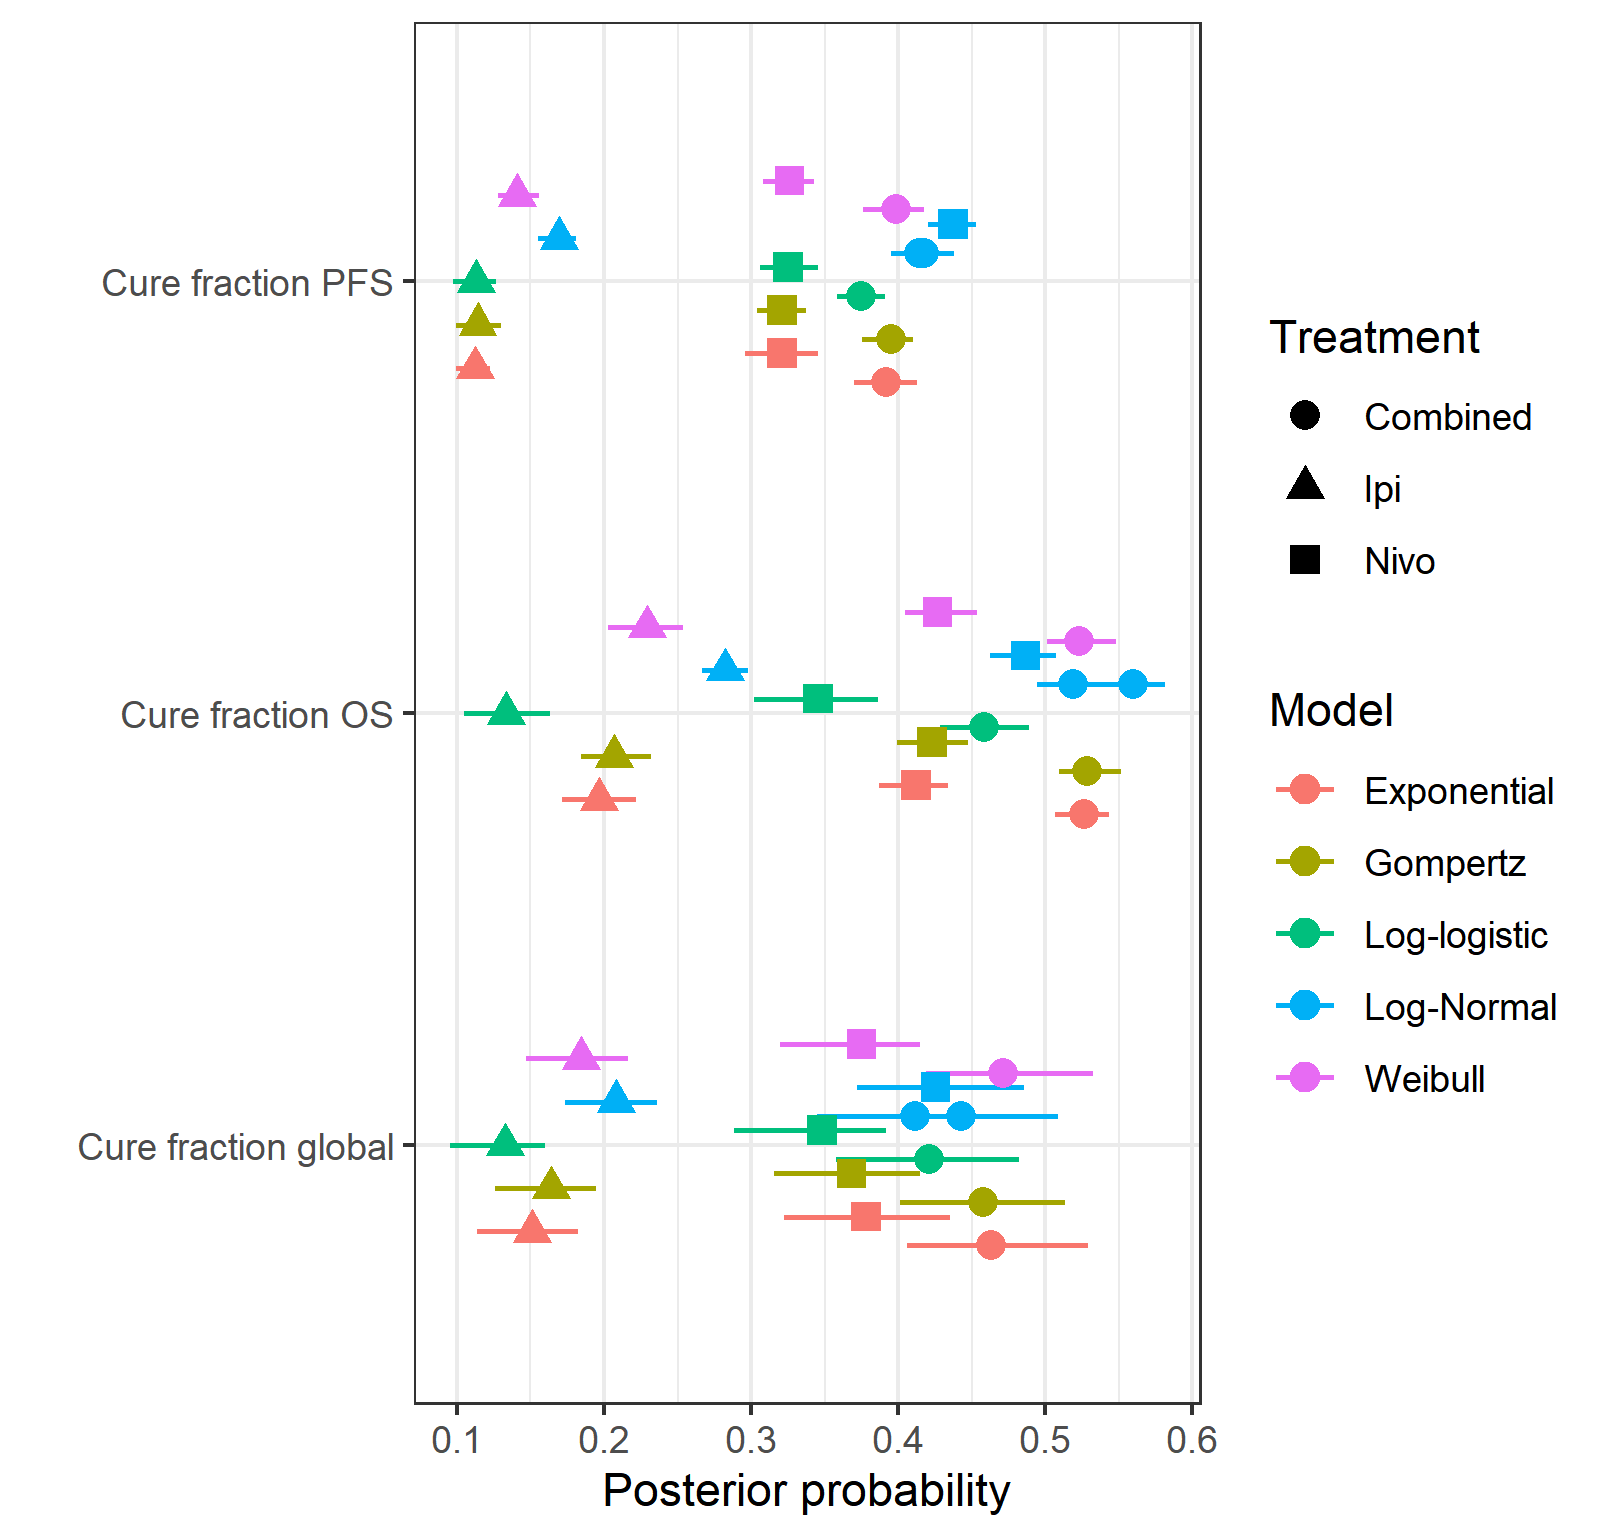
\includegraphics[width=0.6\linewidth]{cf hier_bg_fixed_forest_plot.png}
% \caption{\label{fig:cf_forest} Posterior cure fraction forest plot. Same distributions for OS and PFS. {\it is this how we want to split this up? E.g. do we want different OS and PFS distributions and same treatment? Or separate plots for each cure fraction type?}}
% \end{figure}

% \begin{figure}[H]
% \centering
% 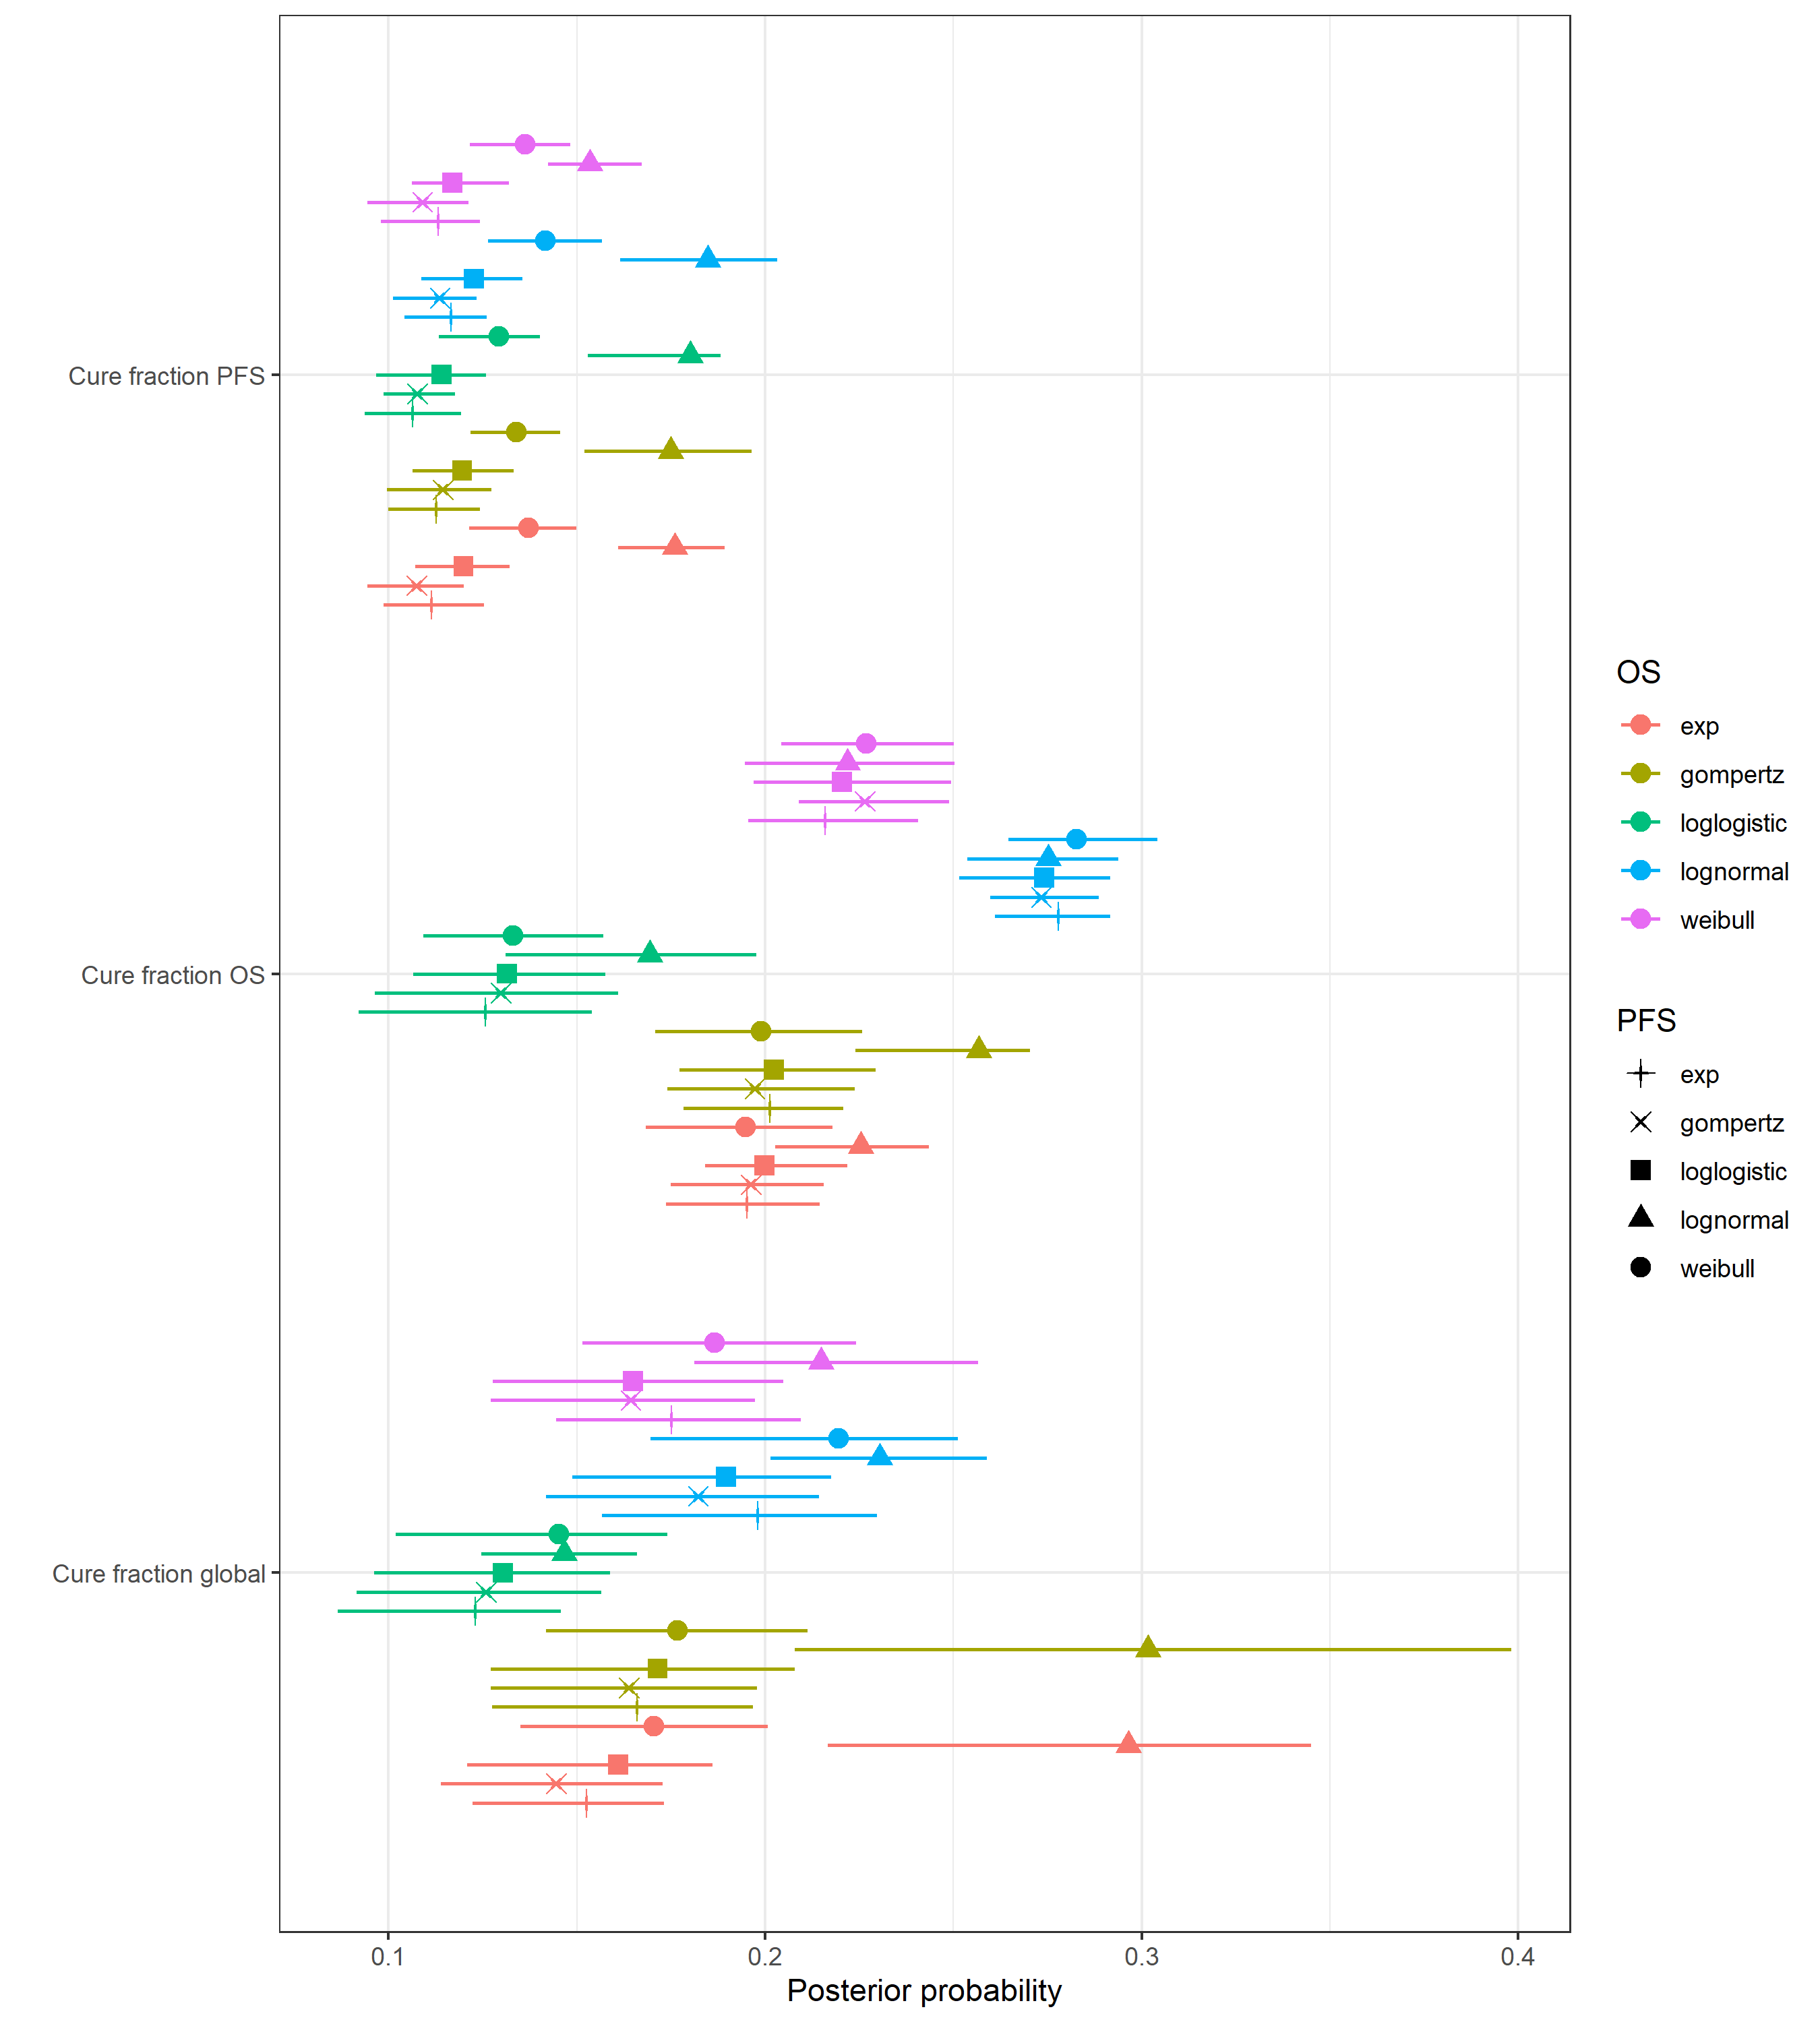
\includegraphics[width=0.6\linewidth]{forest_plot_IPILIMUMAB.png}
% \caption{\label{fig:cf_forest_ipi} Posterior cure fraction forest plot for {\it ipilimumab} treatment.}
% \end{figure}

% \begin{figure}[H]
% \centering
% 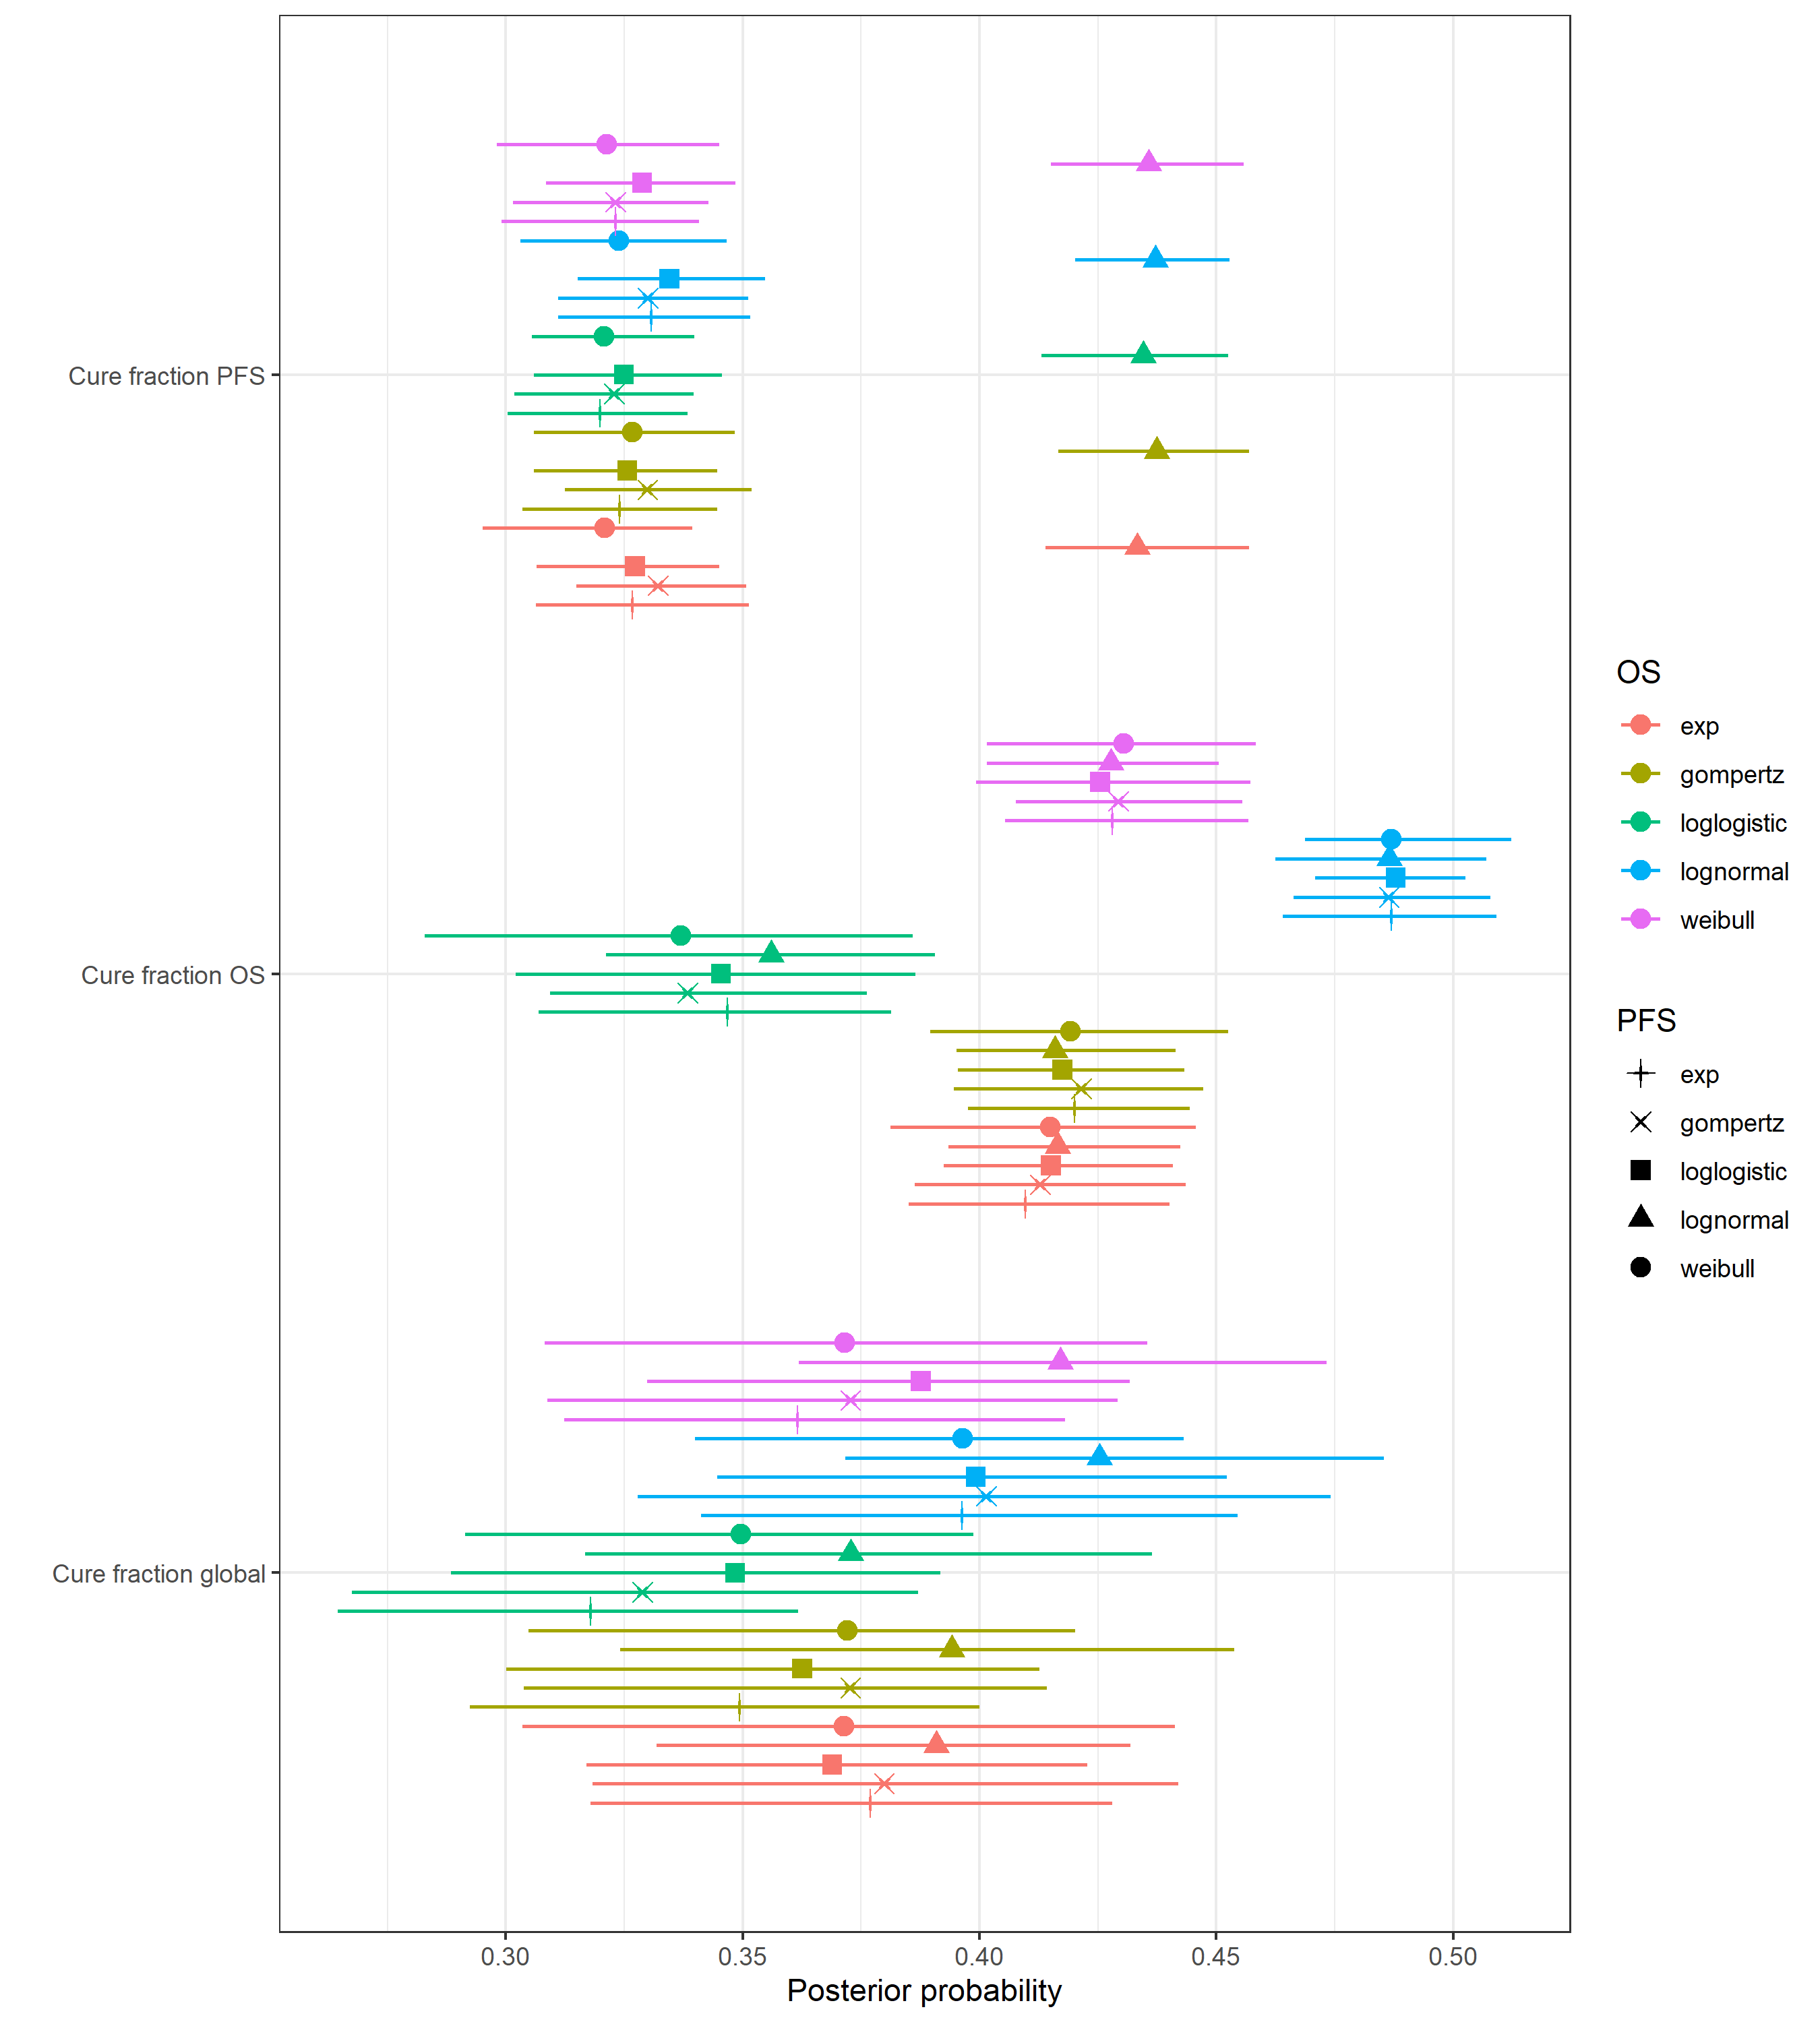
\includegraphics[width=0.6\linewidth]{forest_plot_NIVOLUMAB.png}
% \caption{\label{fig:cf_forest_nivo} Posterior cure fraction forest plot for {\it nivolumab} treatment.}
% \end{figure}

% \begin{figure}[H]
% \centering
% 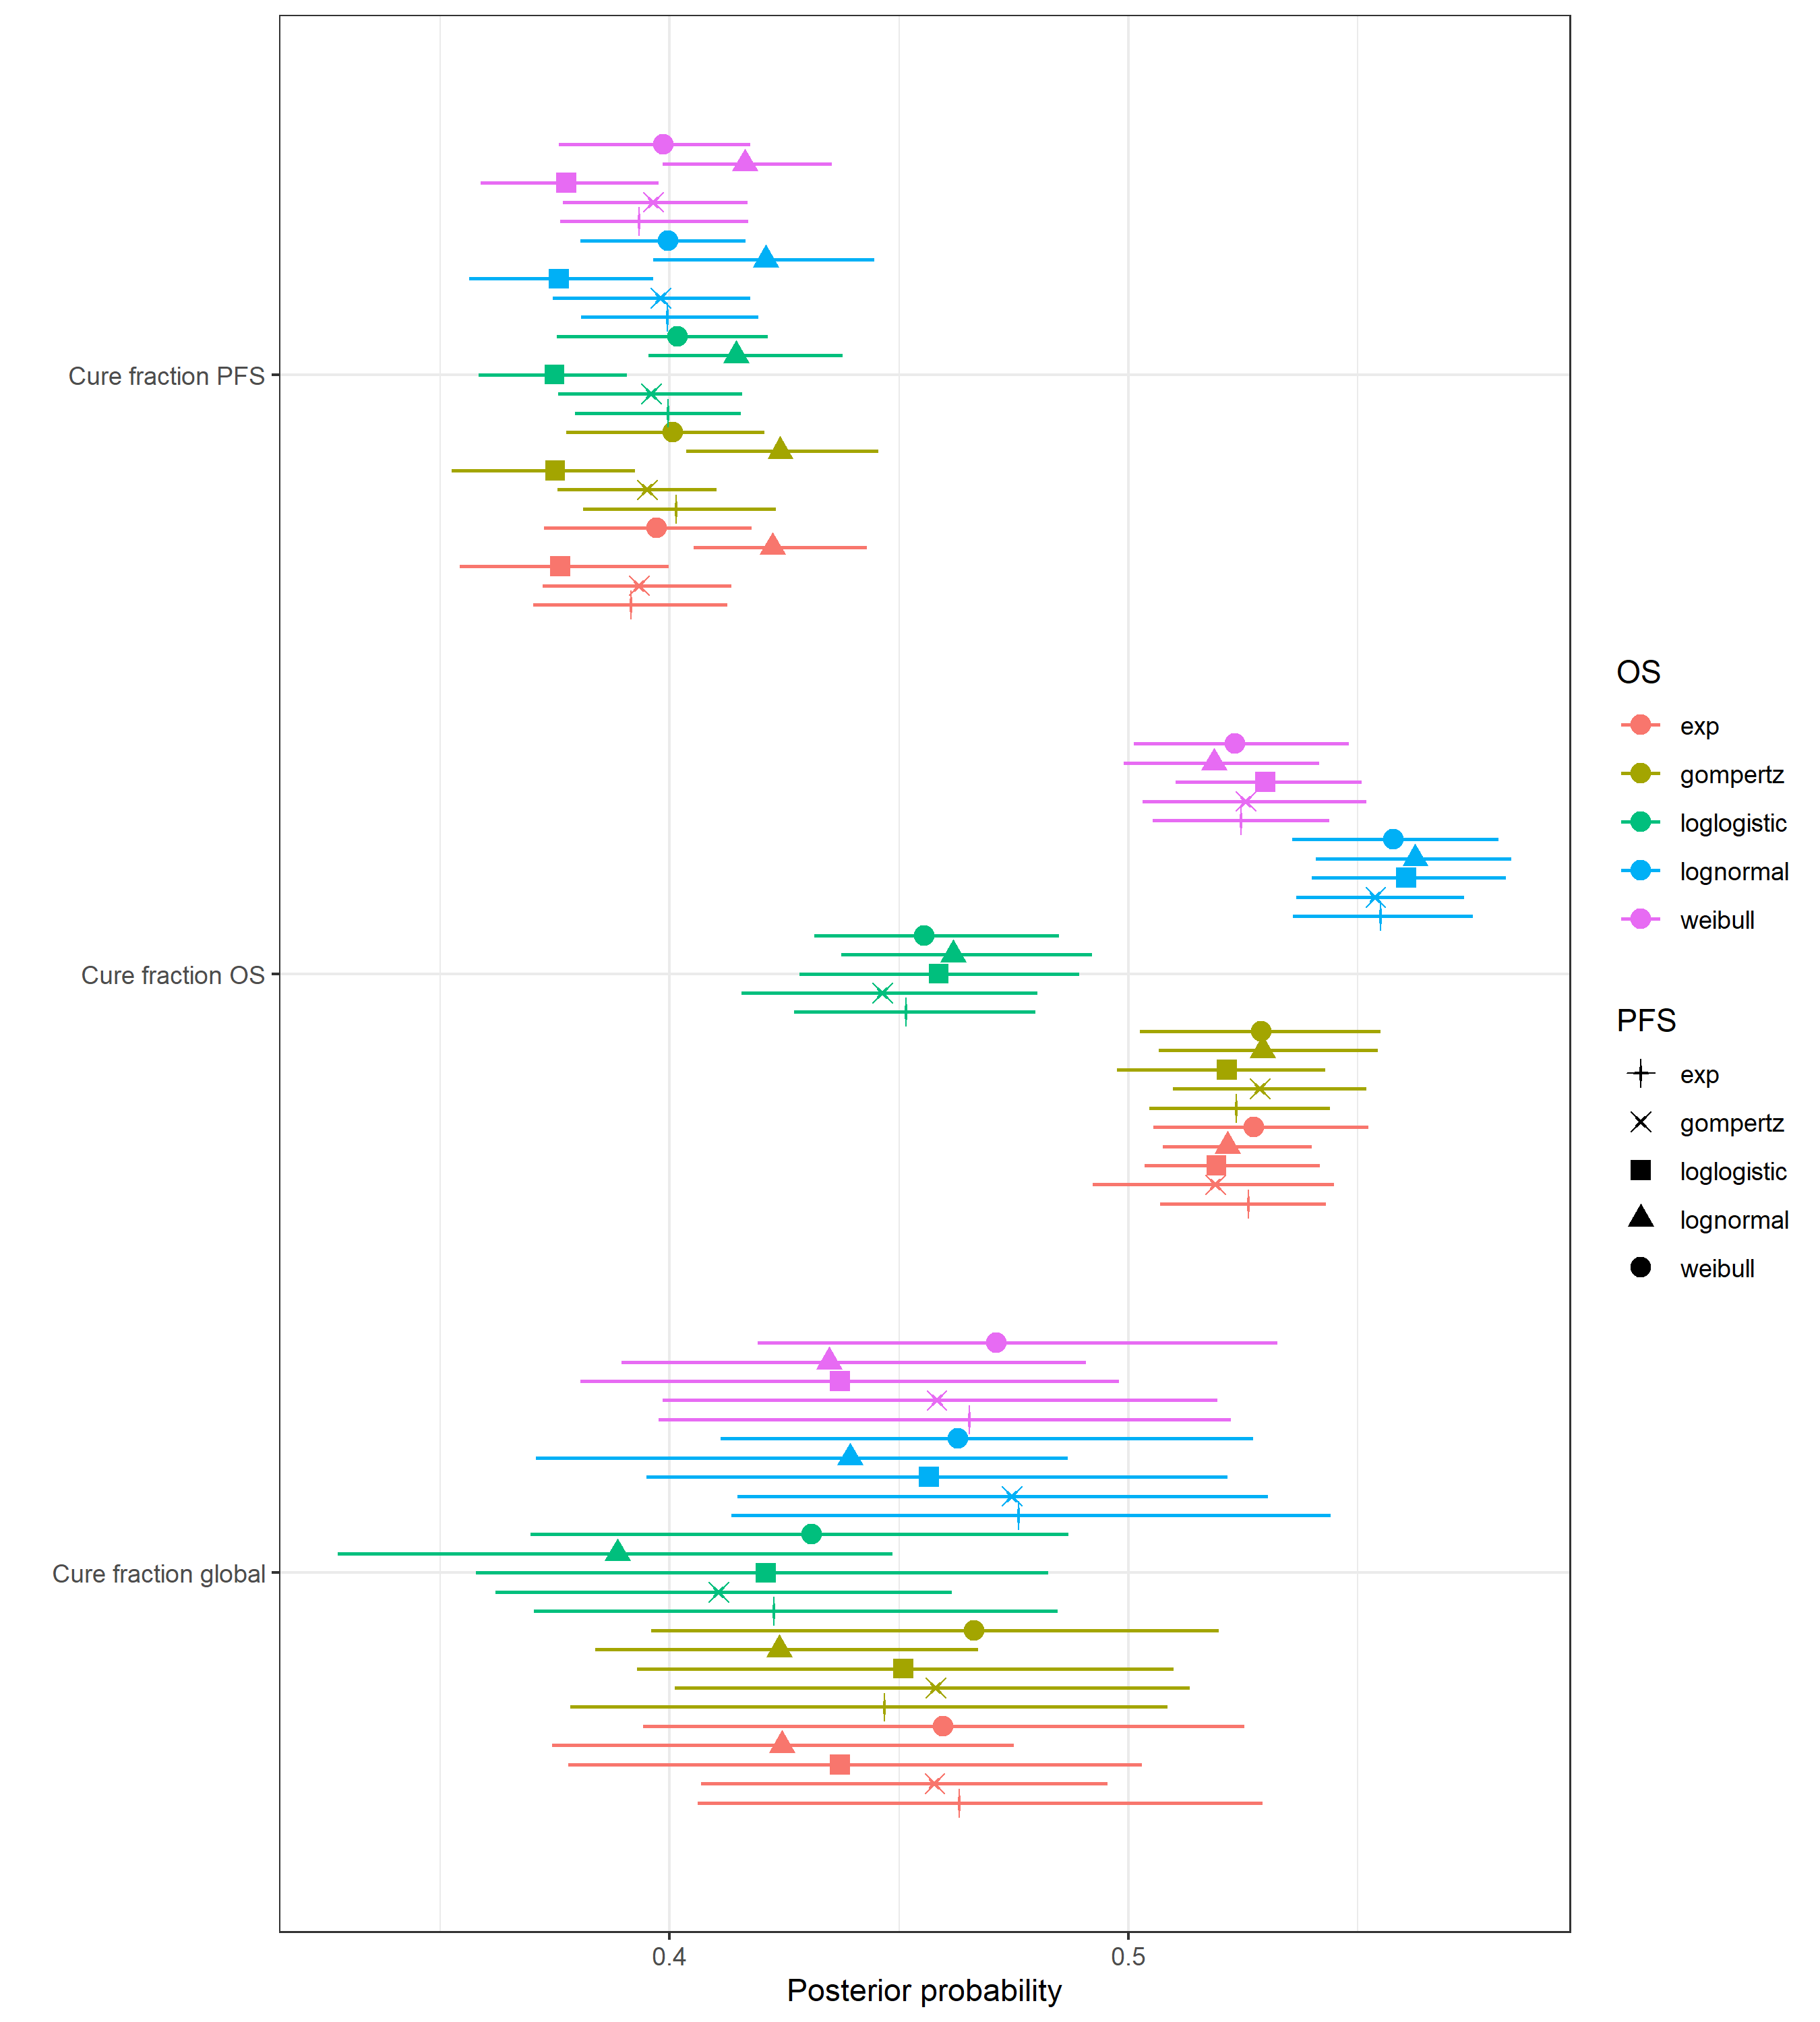
\includegraphics[width=0.6\linewidth]{forest_plot_NIVOLUMAB+IPILIMUMAB.png}
% \caption{\label{fig:cf_forest_ipi_nivo} Posterior cure fraction forest plot for {\it nivolumab} and {\it ipilimumab} combination treatment.}
% \end{figure}

% \begin{sidewaysfigure}[H]
% 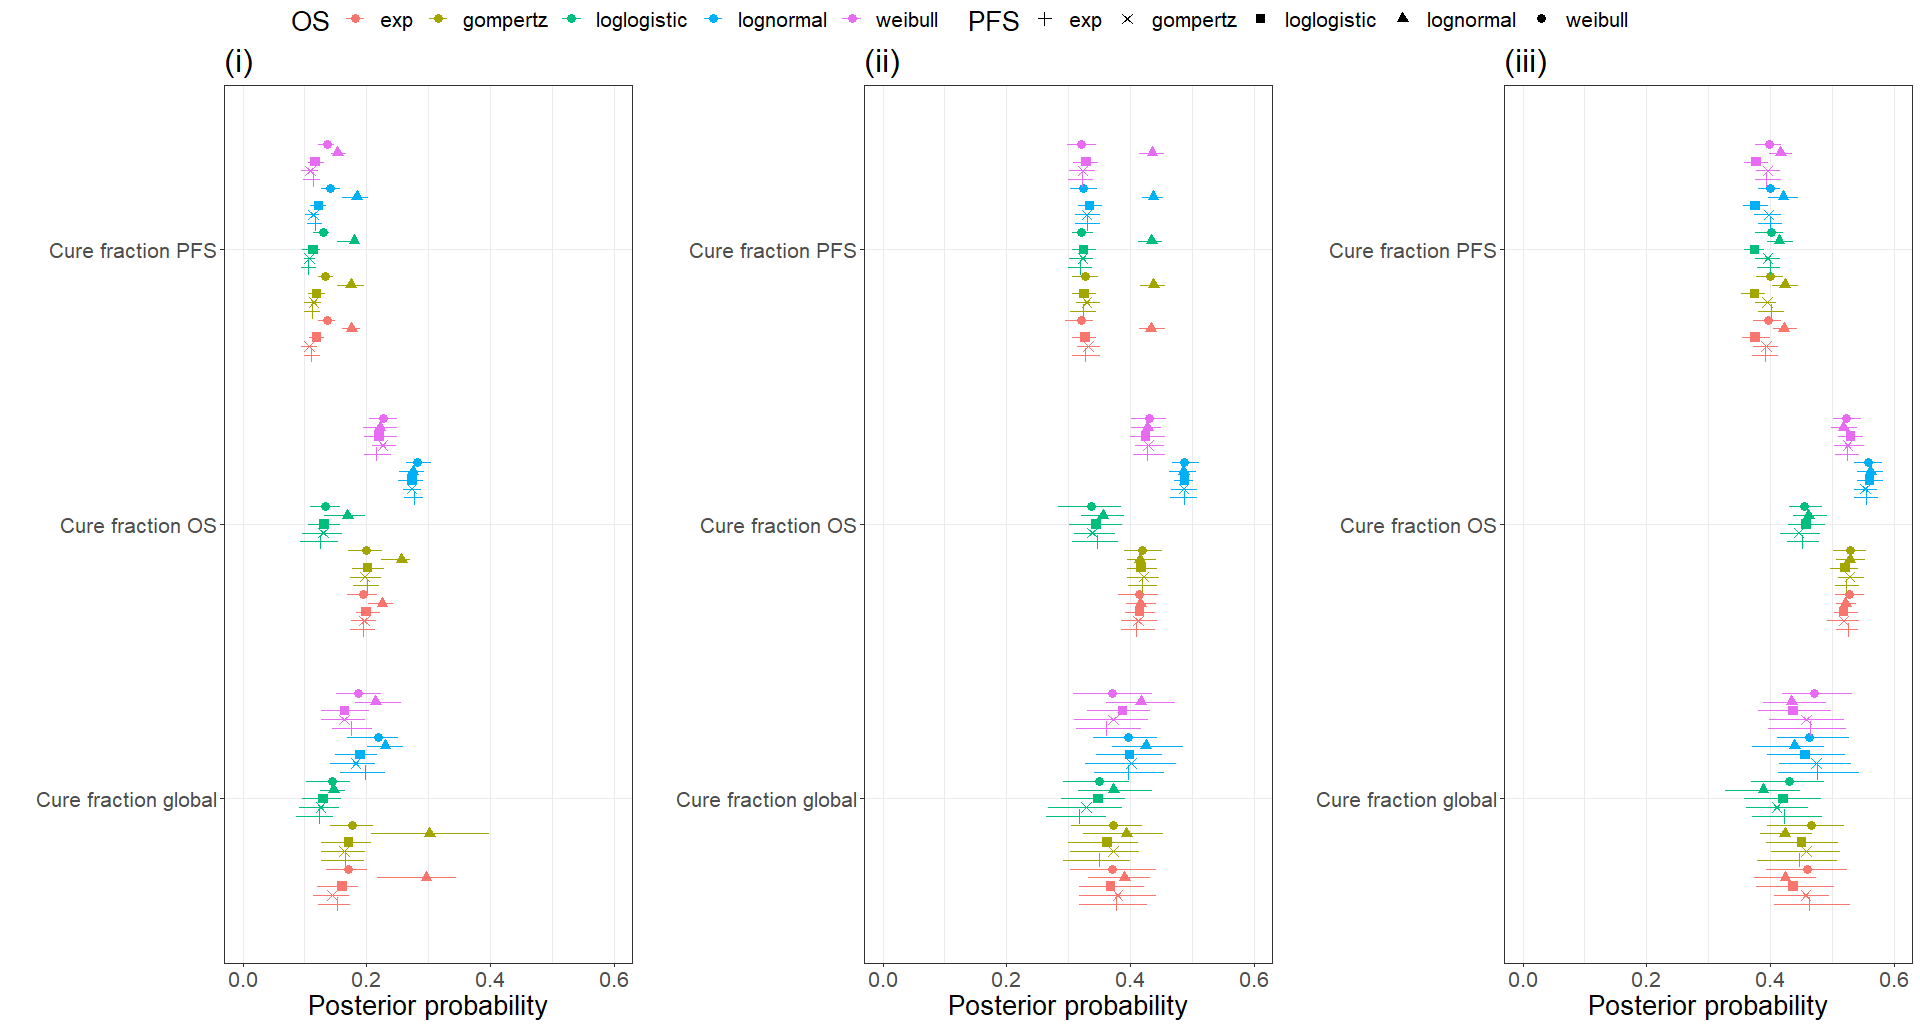
\includegraphics[width=0.9\linewidth]{forest_plot_all_tx.png}
% \caption{\label{fig:cf_forest_all_tx} Posterior cure fraction forest plots for (i) {\it ipilimumab} only (ii) {\it nivolumab} only and (iii) combination treatment.}
% \end{sidewaysfigure}

% \begin{landscape}
% \begin{sidewaysfigure}[H]
\begin{figure}
\centering
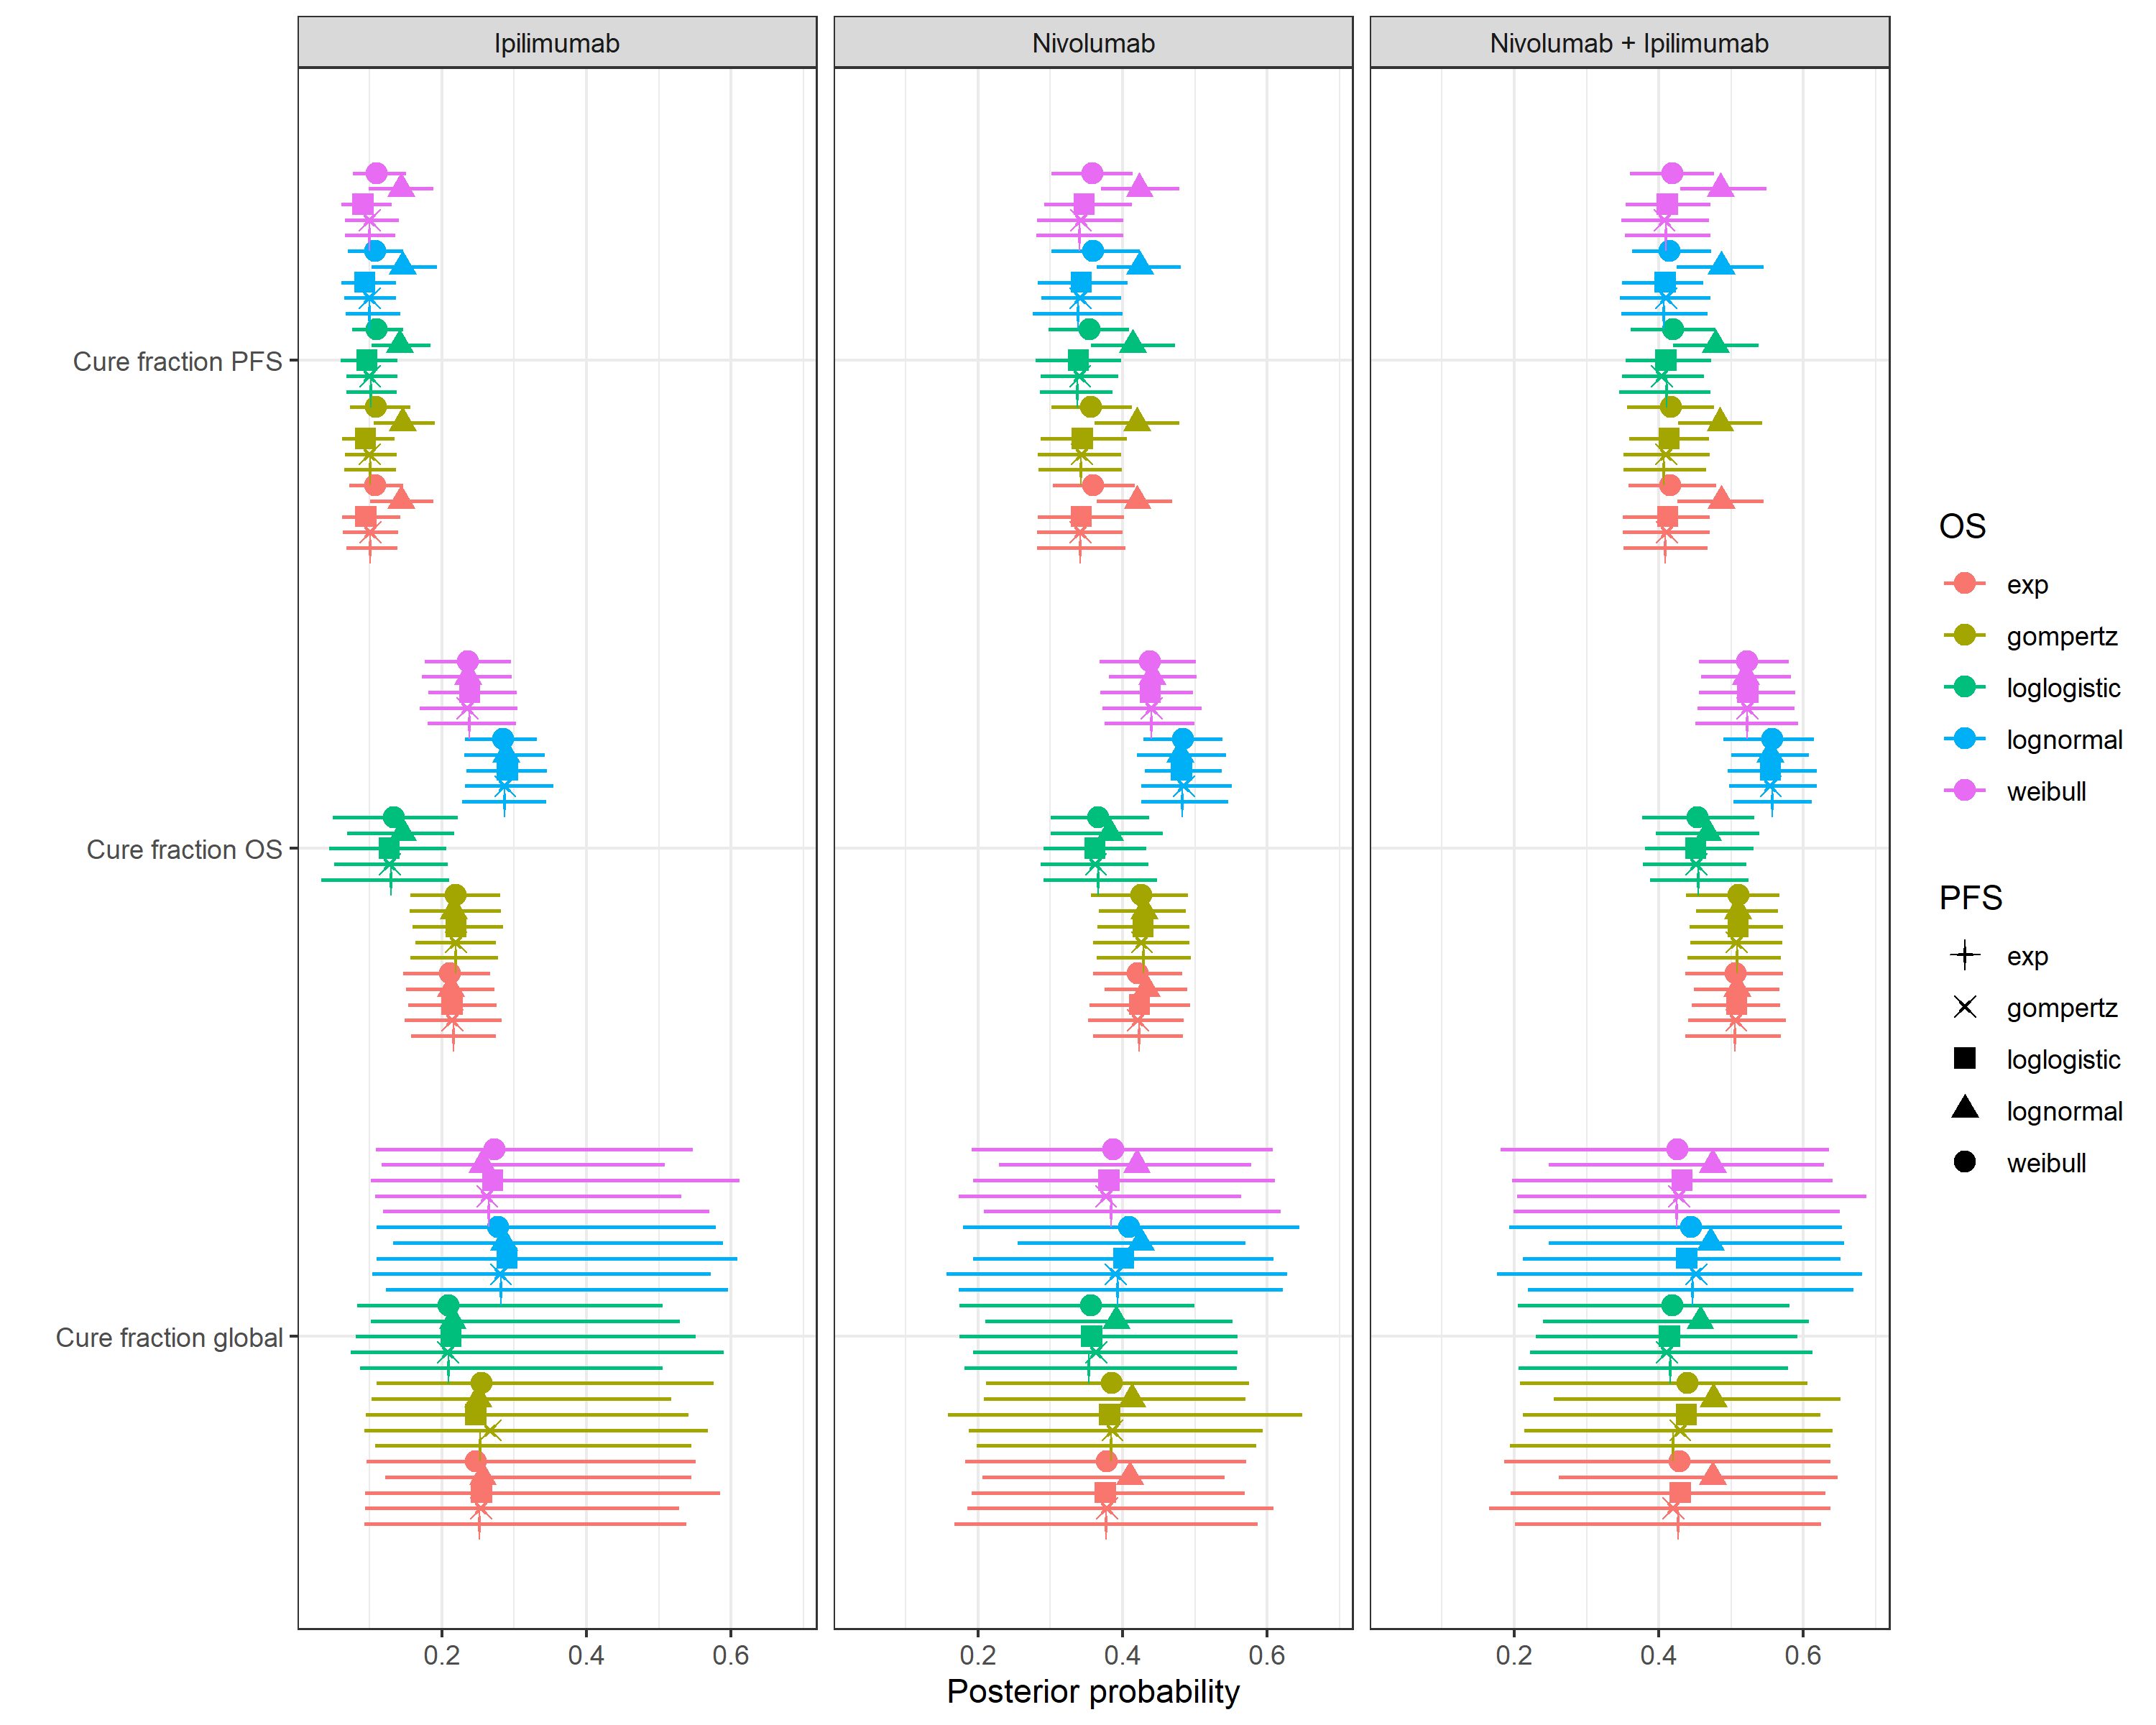
\includegraphics[width=0.9\linewidth]{forest_plot_joint_cf_hier.png}
\caption{\label{fig:cf_forest_all_tx} Hierarchical model posterior cure fraction forest plots with 95\% credible intervals for (i) {\it ipilimumab} only (ii) {\it nivolumab} only and (iii) combination treatment.}
% \end{sidewaysfigure}
\end{figure}
% \end{landscape}

% \begin{landscape}
% \begin{sidewaysfigure}[H]
\begin{figure}
\centering
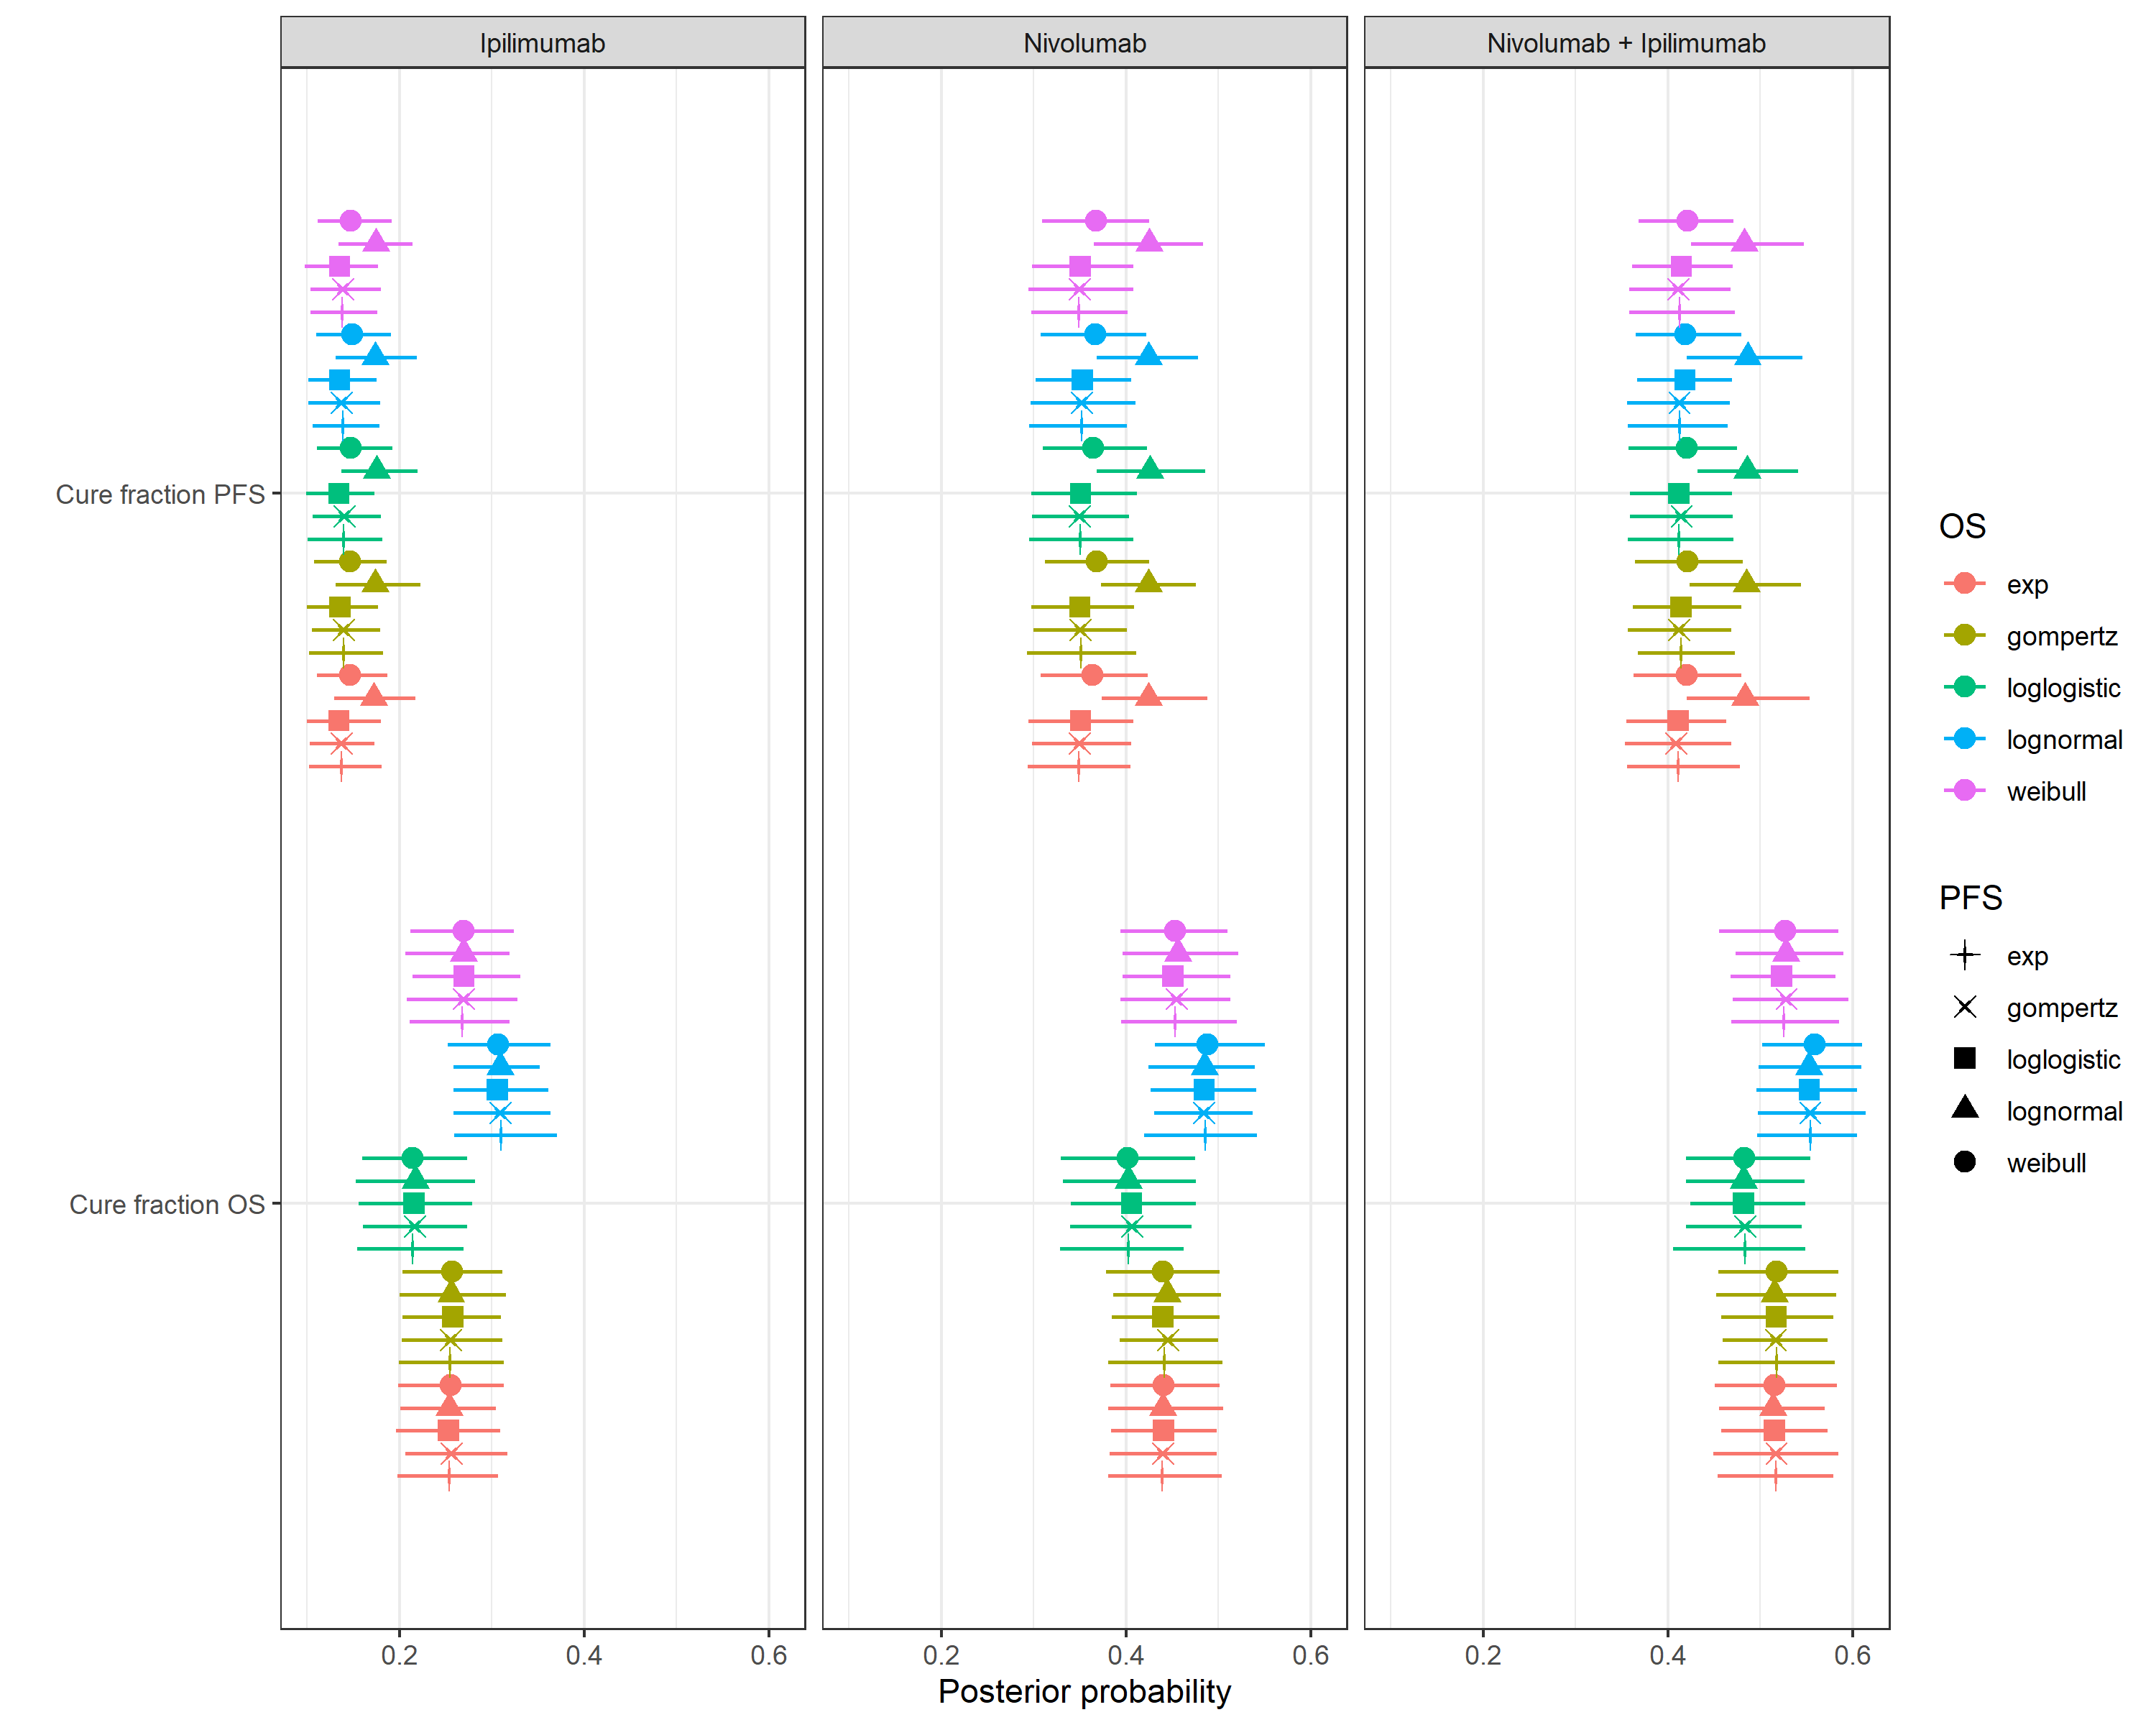
\includegraphics[width=0.9\linewidth]{forest_plot_joint_all_tx_separate.png}
\caption{\label{fig:cf_forest_all_tx_sep} Separate model posterior cure fraction forest plots with 95\% credible intervals for (i) {\it ipilimumab} only (ii) {\it nivolumab} only and (iii) combination treatment.}
% \end{sidewaysfigure}
\end{figure}
% \end{landscape}

The mixed survival curves only show the background mortality survival from when the uncured survival curves meet the x-axis so since this is user-supplied then there is no additional insight. This is the particularly the case for PFS and the log-Normal distribution.


\subsection{Different sample sizes due to cut-point censoring}
Consider that we do not have access to the complete study follow-up data set.
We shall select sensible cut-point times for demonstration purposes at 12 and 30 months.
One of the benefit of adopting a hierarchical Bayesian approach is robustness to smaller sample sizes due to prior information and borrowing of strength.


Stabilisation of the cure fraction
Global cure fraction is stable but uncertain

For separate PFS and OS analysis there are conflicting results.

DIC values for 12 and 30 months are...

For the separate models, for 12 months the exp/exp underestimates the OS cure fraction and then approaches the true value from below for more data.
Whereas the OS cure fraction for log-Normal/log-Normal overestimates the cure fraction 12 months and then approaches the true value (for the complete data set) from above for more data.
These are clearly two very different behaviours but we would not know which is correct until later on in the trial.
Conversely, for the hierarchical model the cure fraction estimate is more stable about the true value.

Figures~\ref{fig:forest_plot_cf_cutpoint_sep} and \ref{fig:forest_plot_cf_cutpoint_hier} show forest plots of the cure fraction estimate for 12, 30 and all months, the exp/exp and log-Normal/log-Normal models and for the separate and hierarchical models respectively.

Figures~\ref{fig:S_cutpoint_12mo_sep} and \ref{fig:S_cutpoint_12mo_hier} show
the survival curves for 12 months of follow-up data for the the exp/exp and log-Normal/log-Normal models and for the separate and hierarchical models respectively.

We can see that in Figure~\ref{fig:forest_plot_cf_cutpoint_sep} for the exp-exp in the OS survival curves for the separate model there is more uncertainty than in the equivalent plot for the hierarchical model in \ref{fig:forest_plot_cf_cutpoint_hier}.

Also, Figure~\ref{fig:forest_plot_cf_cutpoint_sep} for the log-Normal/log-Normal in the OS survival curves for separate and hierarchical models it over-estimates the cure fraction. It appears to revert to the background survival at the time of the last observed data point.

The forest plots demonstrate the same behaviour.
Figure~\ref{fig:S_cutpoint_12mo_sep}
Figure~\ref{fig:S_cutpoint_12mo_hier}


\begin{figure}[!H]
\centering
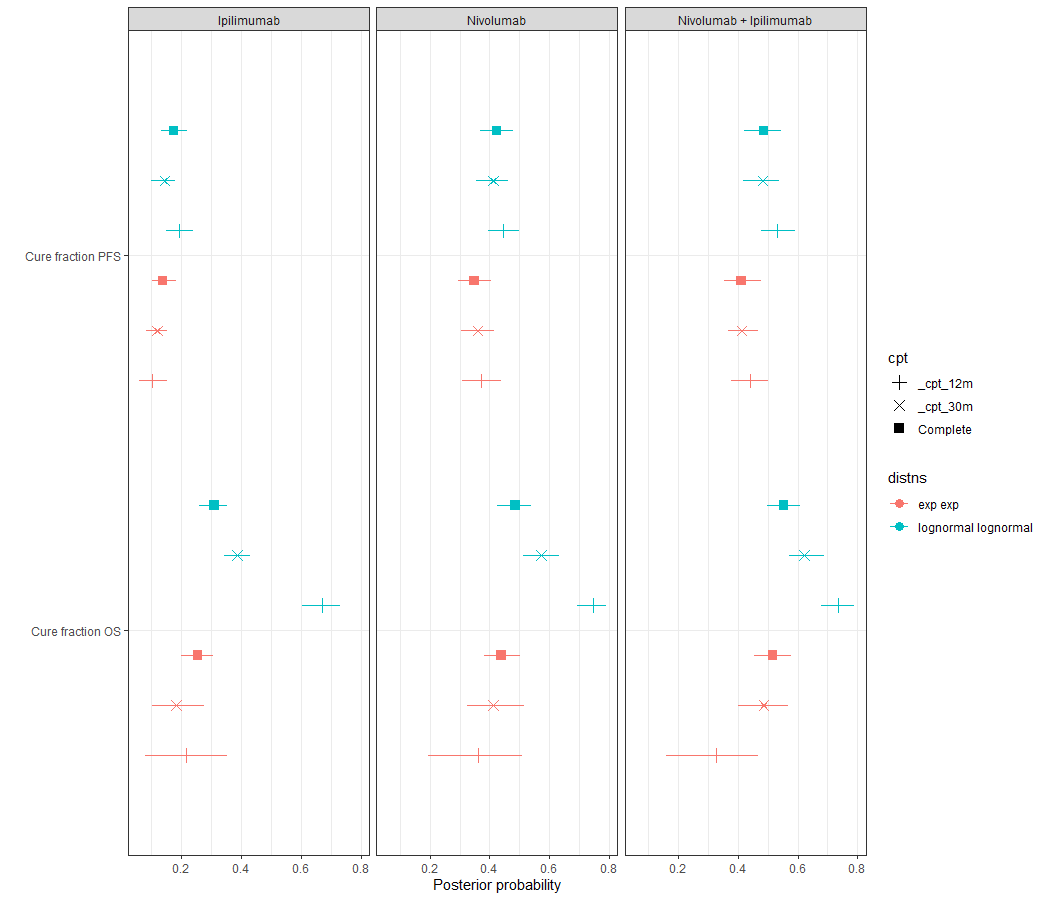
\includegraphics[width=0.6\linewidth]{forest_plot_cf_sep_cpt.png}
\caption{\label{fig:forest_plot_cf_cutpoint_sep} Posterior cure fraction forest plot for study data censored at 12 months, 30 months and the complete data set using the separate model.}
\end{figure}

\begin{figure}[!H]
\centering
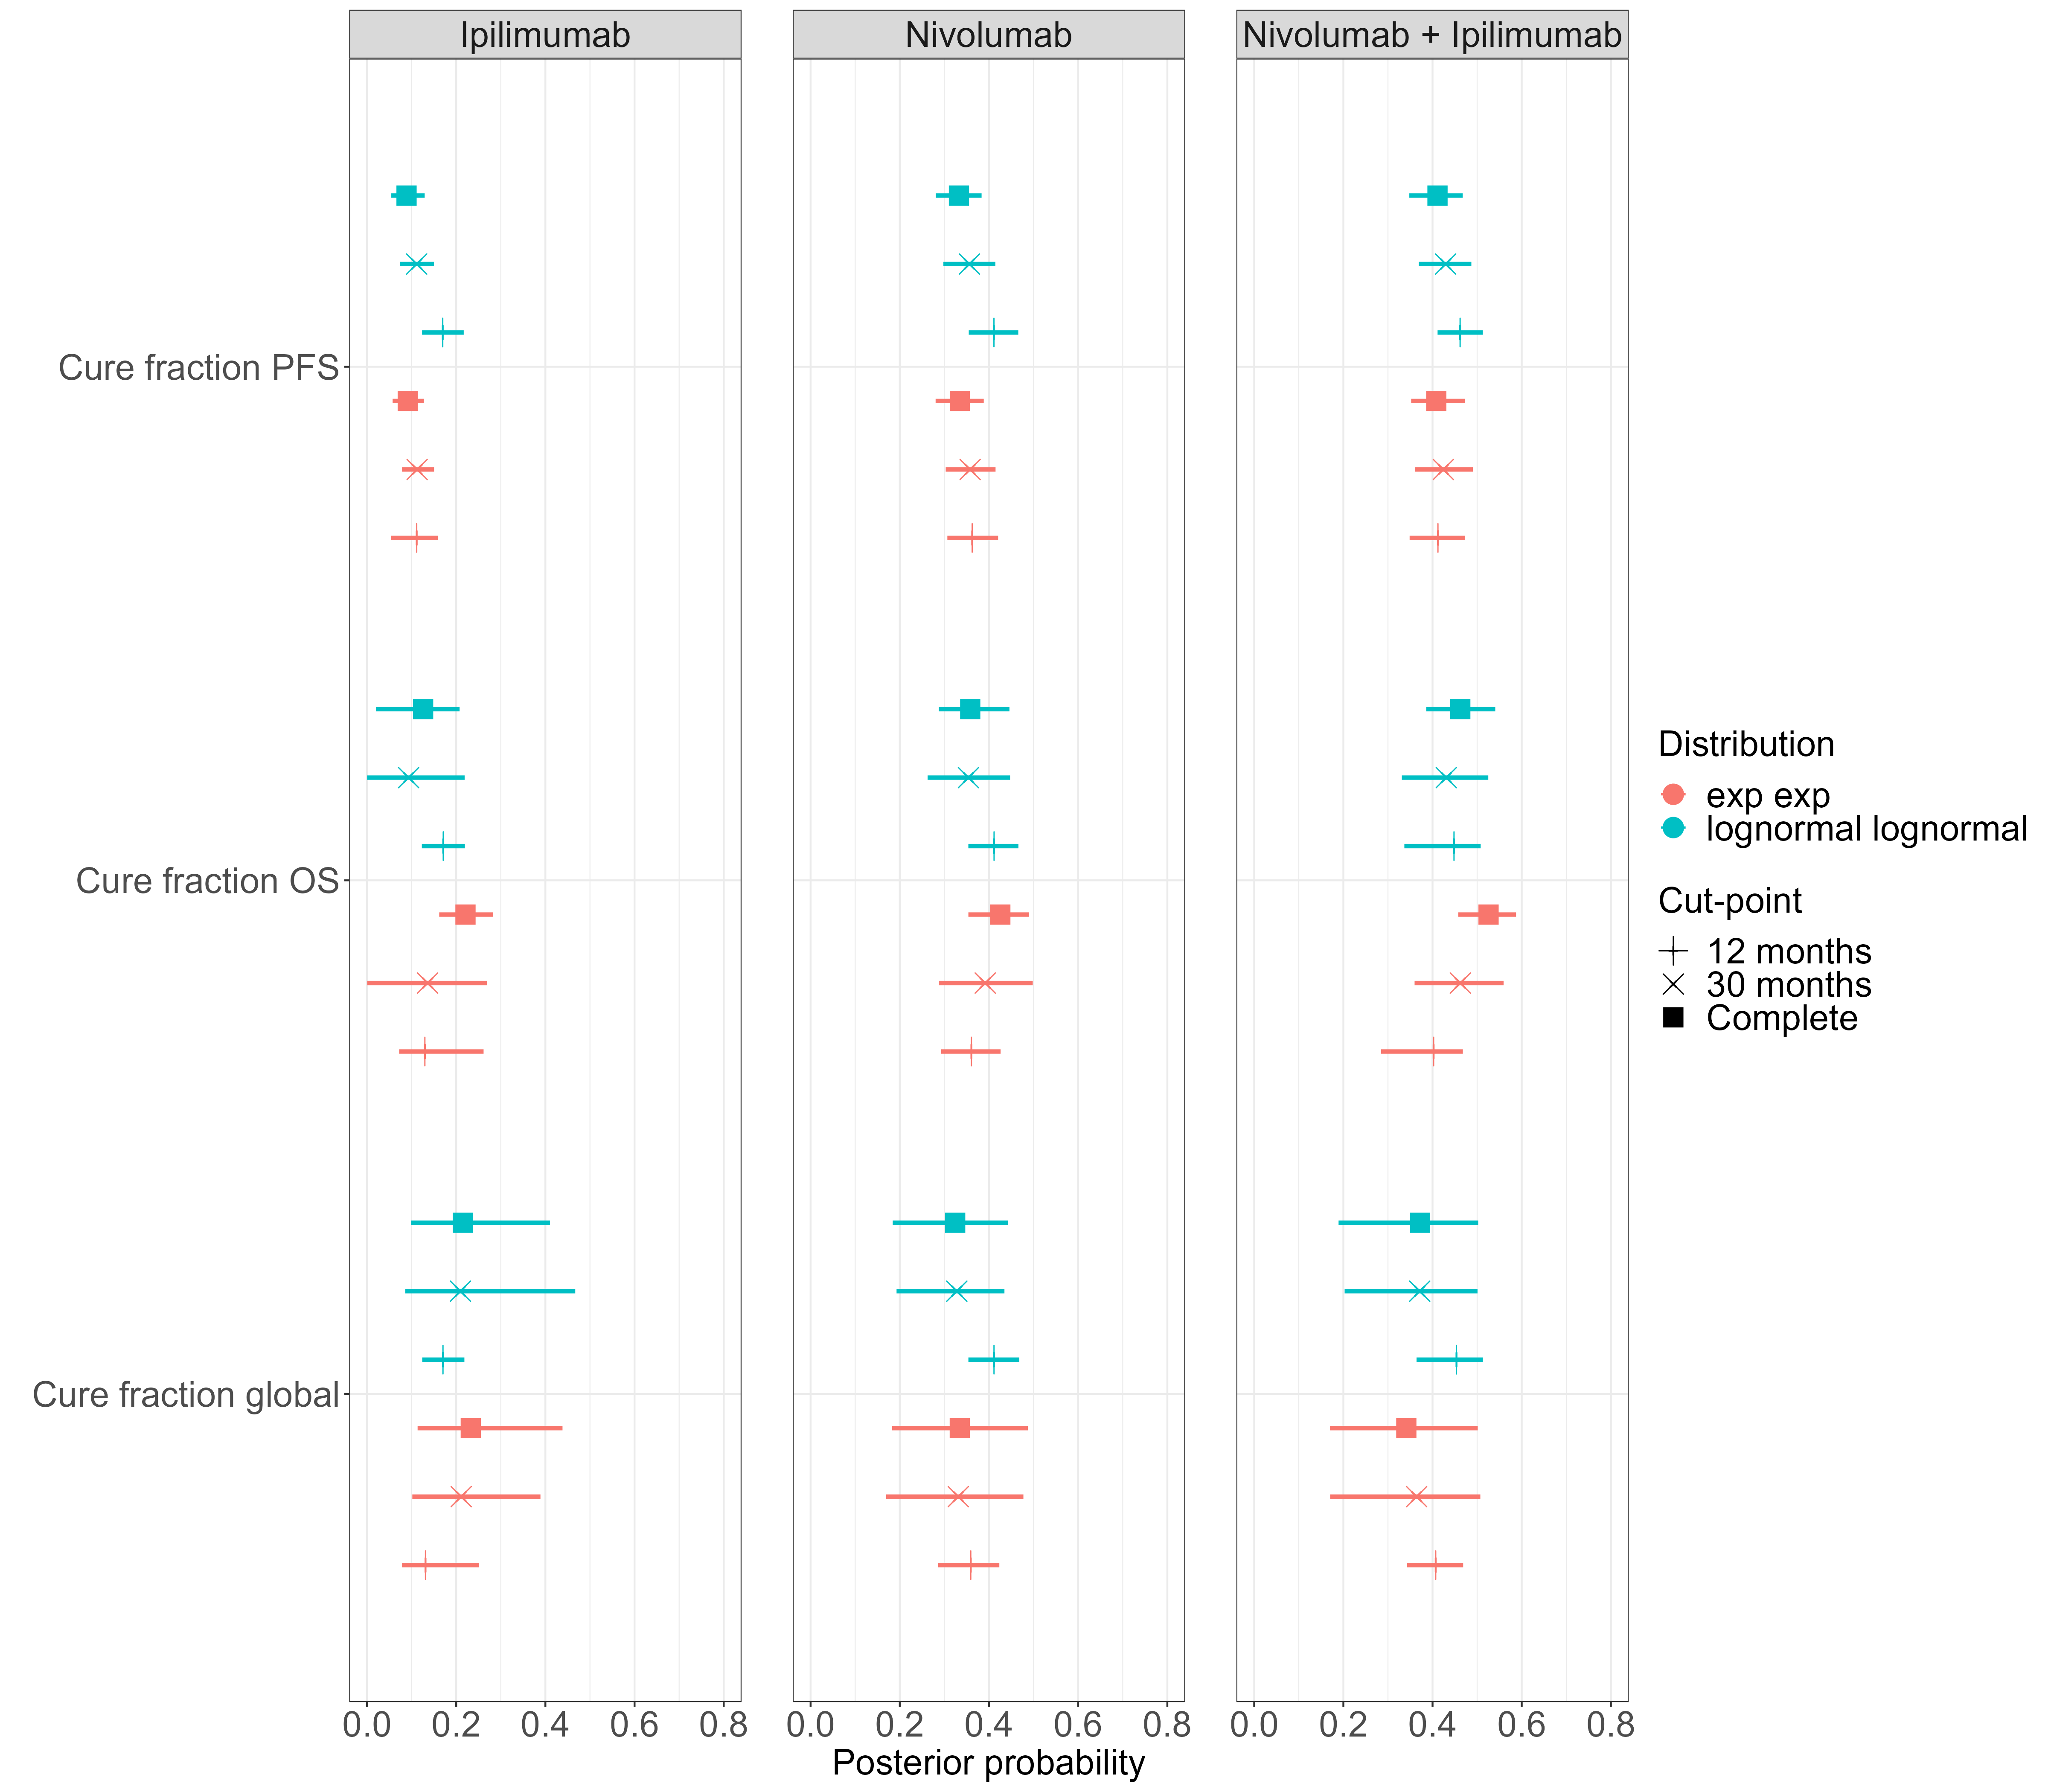
\includegraphics[width=0.6\linewidth]{forest_plot_cf_hier_cpt.png}
\caption{\label{fig:forest_plot_cf_cutpoint_hier} Posterior cure fraction forest plot for study data censored at 12 months, 30 months and the complete data set using the hierarchical model.}
\end{figure}

\begin{figure}[!H]
\centering
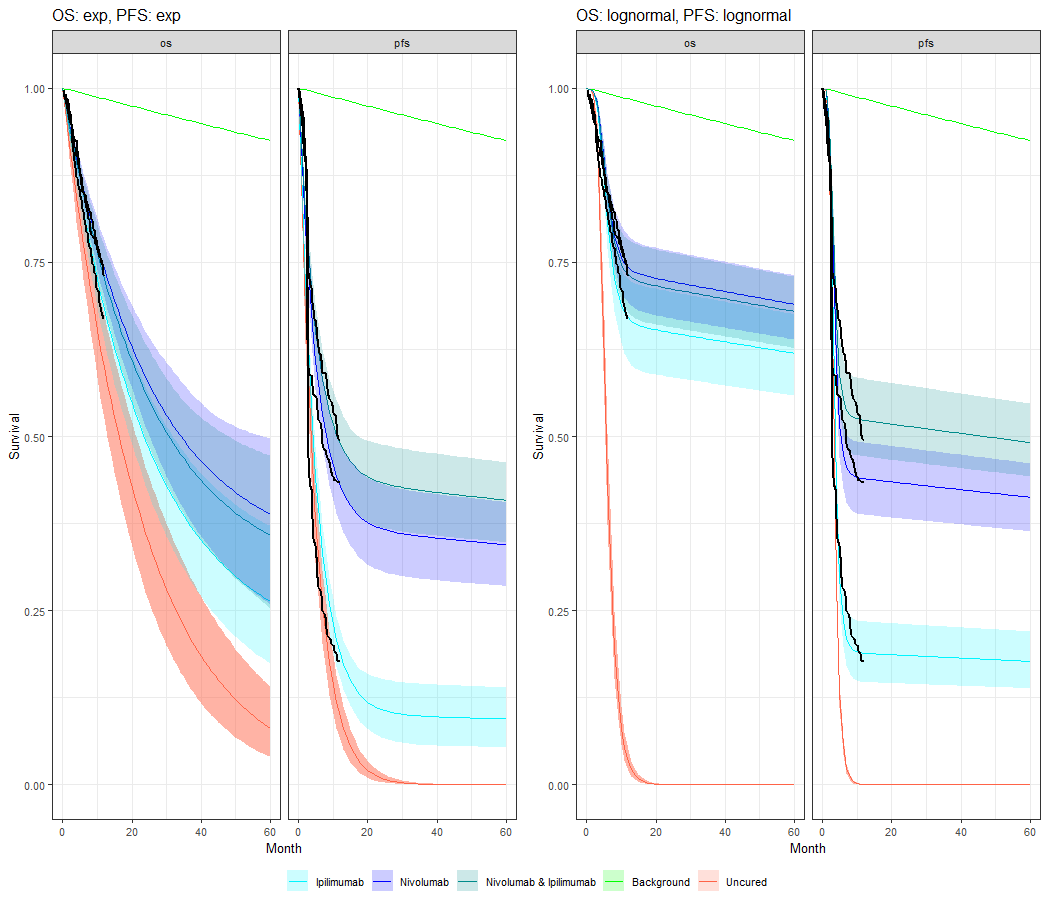
\includegraphics[width=0.6\linewidth]{S_cp_12mo_exp_lognormal_sep.png}
\caption{\label{fig:S_cutpoint_12mo_sep} Separate model posterior survival curves for exponential/exponential and log-Normal/log-Normal uncured fraction for OS/PFS events and censored times at 12 months. The black lines show the observed data Kaplan-Meier curves.}
\end{figure}

\begin{figure}[!H]
\centering
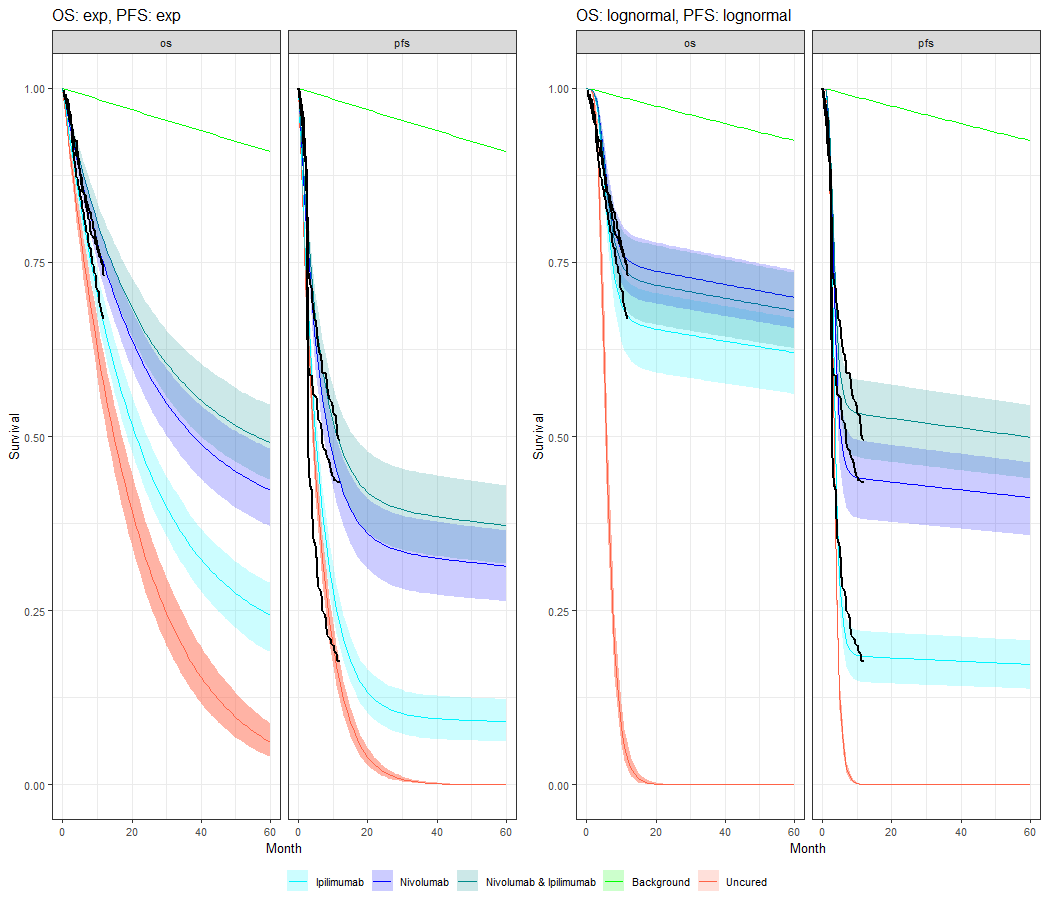
\includegraphics[width=0.6\linewidth]{S_cp_12mo_exp_lognormal_hier.png}
\caption{\label{fig:S_cutpoint_12mo_hier} Hierarchical model posterior survival curves for exponential/exponential and log-Normal/log-Normal uncured fraction for OS/PFS events and censored times at 12 months. The black lines show the observed data Kaplan-Meier curves.}
\end{figure}



\section{Discussion}\label{sec:discussion}

Our approach allows for the incorporation of sensible information.
Stabilise the inference on the cure fraction but restricting/constraining it values via the prior distributions.

% choice of priors
In comparison to some previous frequentist approaches, our framework is able to include contextual information about the parameters of the model via the prior distributions.
For this analysis we chose uninformative priors.
This allows the data to dominate the posterior even if the dataset is relatively small.
In practice there may be additional information from clinical experience or previous data that can better inform the prior selection.
The priors can be specified on the natural scale to aid elicitation and interpretation.
For example, we may have clinical knowledge that a drug treatment could generate a cure fraction greater than, say, 30\%.
If a (cancer) patient enters the study at 60 years old then there is a high degree of certainty that they will not live for, say, over 40 years.
In the case of sparse data e.g. when there is a large amount of missing data perhaps due to right censoring, then 'regularising' the inference based on available prior information could make a significant and important difference.

How to elicit this prior information in practice may not be simple and a formal protocol should be adopted \cite{OHagan2019}.


The regulators may value the fact that a hierarchical model can embed some form of prior knowledge to account for scepticism.
This will prevent the cure rates to be taken at face value, particularly with limited data.
The hierarchical model seems to give a more precise estimate of the cure rate, even with earlier data cuts (especially for the Exponential model).
The hierarchical model is more aligned, which means possibly you have more reliable estimates early on, which is a good argument to complement modelling based on earlier cuts.
Earlier cuts can lead to quicker introduction in the market and reimbursement decisions.

% optimal stopping
Another way to think about the cut-point data is to think about what time should we choose to halt the trial and end the data collection which would maximise some expected overall utility.
That is what is the optimal stopping time $\tau^*$ for the total utility $V$.
$$
\mathbb{E} V_{\tau^*} = \sup_{\tau} \mathbb{E} V_{\tau}
$$
The stopping utility may include benefits such as smaller costs, freed-up time from the trial for patients and those running the study, quicker time to market for a drug, avoidance of side-effects etc.
The utility would also depend on estimating 'correct' parameters values from the available data i.e. that they are within some acceptable threshold of the true values.
This could be directly on the parameters of interest or an order statistics for which drug is deemed the preferable.

This may be framed in terms of value of information (VoI) [ref].
For example, in the case given above, what is the additional value of obtaining further data after 12 and 30 months.

In practice, deriving a set of heuristics may be better than formalising a general rule.
A discrete set of cut-point may be used, similar to our selection of 12 and 30 months, rather than considering the whole real line.

% use in cost-effectiveness models
An important use of the output from this work is in cost-effectiveness analysis.
The survival times are use directly as an effectiveness measure or in a function to obtain e.g. QALYS or QALE. For unstable cure fraction estimates, such as was the case for a small sample of data for OS in the separate model, would give very different QALY estimates and thus cost-effectiveness statistics and potentially differing optimal decisions.
The hierarchical model, which exhibited more stable estimation, would be more reliable in this situation.


{\it how should the complete responders be included in the main model? If they enter via the background adjustment why double-count them? Landmarking?}

% model structure
It may be that there is excessive borrowing of information between cure fractions when the event types are distinctly different.
In our example, this is not necessary since there are only two event types but for a larger number this may be appropriate.
Partial-exchangeability can be used instead in this case \cite{Neuenschwander2016}.

In terms of an outcome of interest and a surrogate end-point Papanikos~(2020) \cite{Papanikos2020} modelled their relationship using a Bivariate Normal distribution.
We could have done something similar for the OS and PFS event times, especially since the latter is a lower bound for the former.

{\it model averaging using all distributions and weights from LOO/WAIC?}

{\it extensions of the implementation could be to generalise to have different distributions for each treatment in a single model fit, rather than at the moment where they are assumed to be the same for all treatments.}


%\backmatter

\section*{Acknowledgements}
This is acknowledgement text.

\subsection*{Author contributions}

This is an author contribution text.

\subsection*{Financial disclosure}

None reported.

\subsection*{Conflict of interest}

The authors declare no potential conflict of interests.


% \section*{Supporting information}

% The following supporting information is available as part of the online article:

\appendix

\section{Posterior parameter statistics \label{app1}}


% \begin{center}
% \begin{table*}[t]
% \caption{Posterior summary statistics separate treatment models \label{tab:posterior}}
% \centering
% \begin{tabular}{llll}
% \toprule
% Variable & IPILIMUMAB & NIVOLUMAB & NIVOLUMAB+IPILIMUMAB\\
% \midrule
% $\beta^{os}_0$ & -3.167 (-3.408, -2.947) & -3.157 (-3.476, -2.899) & -2.922 (-3.219, -2.657)\\
% $\beta^{os}_1$ & -0.014 (-0.025, -0.002) & -0.014 (-0.029, 0.004) & -0.012 (-0.036, 0.012)\\
% $\beta^{pfs}_0$ & 1.575 (1.471, 1.672) & 1.985 (1.798, 2.148) & 2.014 (1.847, 2.206)\\
% $\beta^{pfs}_1$ & -0.005 (-0.012, 0.001) & 0.013 (0.003, 0.023) & -0.001 (-0.01, 0.008)\\
% $\pi_{global}$ & 0.17 (0.09, 0.291) & 0.371 (0.205, 0.568) & 0.46 (0.271, 0.659)\\
% $\pi_{os}$ & 0.195 (0.148, 0.253) & 0.415 (0.34, 0.485) & 0.527 (0.458, 0.591)\\
% $\pi_{pfs}$ & 0.137 (0.102, 0.185) & 0.321 (0.262, 0.386) & 0.397 (0.34, 0.46)\\
% \bottomrule
% \end{tabular}
% \begin{tablenotes}%%[341pt]
% \item Source: Example for table source text.
% \item[1] Example for a first table footnote.
% \item[2] Example for a first table footnote.
% \end{tablenotes}
% \end{table*}
% \end{center}


%%%%%%%%%%%%%%%%%%
% hierarchical

\begin{landscape}
% \begin{sidewaystable}[H]
\begin{center}
\begin{table*}[t]
\caption{Posterior summary statistics for hierarchical model parameters and all OS distributions with exponential PFS distribution. \label{tab:post_hier_pfs_exp}}
\centering
\begin{tabular}{l c c c c c c c c c c c c c c c}
\toprule
\multicolumn{1}{l}{} & \multicolumn{2}{c}{$\textbf{Exp/Exp}^1$} & & \multicolumn{2}{c}{\textbf{Weibull/Exp}} & & \multicolumn{2}{c}{\textbf{Gompertz/Exp}} & & \multicolumn{2}{c}{\textbf{Log-logistic/Exp}} & & \multicolumn{2}{c}{\textbf{log-Normal/Exp}}\\
\cmidrule{2-3}\cmidrule{5-6}\cmidrule{8-9}\cmidrule{11-12}\cmidrule{14-15}
\textbf{Parameter} & \textbf{Mean} & \textbf{95\% CrI} & & \textbf{Mean} & \textbf{95\% CrI} & & \textbf{Mean} & \textbf{95\% CrI} & & \textbf{Mean} & \textbf{95\% CrI} & & \textbf{Mean} & \textbf{95\% CrI}\\
\midrule
$\beta_{os, 0}$ & -3.093 & (-3.249, -2.956) &  & 3.032 & (2.903, 3.221) &  & -3.094 & (-3.264, -2.948) &  & 2.831 & (2.659, 3.023) &  & 2.478 & (2.406, 2.559) & \\
$\beta_{os, 1}$ & -0.014 & (-0.023, -0.005) &  & 0.011 & (0.003, 0.021) &  & -0.014 & (-0.024, -0.003) &  & 0.011 & (0, 0.021) &  & 0.001 & (-0.004, 0.006) & \\
$\beta_{pfs, 0}$ & -1.825 & (-1.939, -1.728) &  & -1.828 & (-1.925, -1.738) &  & -1.827 & (-1.92, -1.73) &  & -1.831 & (-1.921, -1.734) &  & -1.831 & (-1.924, -1.732) & \\
$\beta_{pfs, 1}$ & -0.003 & (-0.009, 0.004) &  & -0.003 & (-0.009, 0.003) &  & -0.003 & (-0.01, 0.003) &  & -0.003 & (-0.009, 0.003) &  & -0.003 & (-0.009, 0.004) & \\
$\beta^{\pi}_1$ & -1.179 & (-2.283, 0.153) &  & -1.102 & (-2.009, 0.28) &  & -1.168 & (-2.115, 0.18) &  & -1.447 & (-2.351, 0.022) &  & -1.005 & (-1.966, 0.386) & \\
$\beta^{\pi}_2$ & -0.527 & (-1.604, 0.351) &  & -0.494 & (-1.337, 0.485) &  & -0.496 & (-1.4, 0.341) &  & -0.625 & (-1.509, 0.231) &  & -0.463 & (-1.565, 0.498) & \\
$\beta^{\pi}_3$ & -0.311 & (-1.382, 0.508) &  & -0.324 & (-1.392, 0.62) &  & -0.348 & (-1.422, 0.565) &  & -0.354 & (-1.35, 0.318) &  & -0.228 & (-1.269, 0.706) & \\
$\sigma_1$ & 1.403 & (0.339, 3.87) &  & 1.486 & (0.325, 4.266) &  & 1.542 & (0.302, 4.395) &  & 1.268 & (0.058, 4.274) &  & 1.514 & (0.399, 3.907) & \\
$\sigma_2$ & 0.791 & (0.056, 2.834) &  & 0.868 & (0.111, 3.433) &  & 0.846 & (0.064, 2.911) &  & 0.701 & (0.012, 2.897) &  & 1.132 & (0.197, 4.121) & \\
$\sigma_3$ & 0.852 & (0.091, 2.636) &  & 0.985 & (0.146, 3.444) &  & 1.008 & (0.116, 3.424) &  & 0.703 & (0.016, 2.906) &  & 1.102 & (0.213, 3.506) & \\
$\pi_{global, 1}$ & 0.252 & (0.093, 0.538) &  & 0.265 & (0.118, 0.57) &  & 0.253 & (0.108, 0.545) &  & 0.209 & (0.087, 0.505) &  & 0.282 & (0.123, 0.595) & \\
$\pi_{global, 2}$ & 0.377 & (0.167, 0.587) &  & 0.384 & (0.208, 0.619) &  & 0.384 & (0.198, 0.584) &  & 0.354 & (0.181, 0.557) &  & 0.393 & (0.173, 0.622) & \\
$\pi_{global, 3}$ & 0.427 & (0.201, 0.624) &  & 0.425 & (0.199, 0.65) &  & 0.420 & (0.194, 0.638) &  & 0.416 & (0.206, 0.579) &  & 0.447 & (0.219, 0.67) & \\
$\pi_{os, 1}$ & 0.216 & (0.158, 0.275) &  & 0.238 & (0.181, 0.302) &  & 0.219 & (0.156, 0.278) &  & 0.130 & (0.033, 0.211) &  & 0.286 & (0.228, 0.344) & \\
$\pi_{os, 2}$ & 0.423 & (0.359, 0.484) &  & 0.440 & (0.375, 0.499) &  & 0.429 & (0.364, 0.494) &  & 0.366 & (0.291, 0.447) &  & 0.483 & (0.426, 0.546) & \\
$\pi_{os, 3}$ & 0.505 & (0.437, 0.569) &  & 0.523 & (0.45, 0.593) &  & 0.508 & (0.439, 0.569) &  & 0.455 & (0.388, 0.524) &  & 0.557 & (0.503, 0.611) & \\
$\pi_{pfs, 1}$ & 0.101 & (0.068, 0.139) &  & 0.099 & (0.065, 0.135) &  & 0.100 & (0.065, 0.137) &  & 0.102 & (0.068, 0.137) &  & 0.099 & (0.067, 0.142) & \\
$\pi_{pfs, 2}$ & 0.341 & (0.282, 0.404) &  & 0.340 & (0.281, 0.401) &  & 0.342 & (0.284, 0.398) &  & 0.338 & (0.285, 0.386) &  & 0.338 & (0.276, 0.4) & \\
$\pi_{pfs, 3}$ & 0.409 & (0.351, 0.468) &  & 0.410 & (0.353, 0.472) &  & 0.407 & (0.351, 0.466) &  & 0.411 & (0.345, 0.472) &  & 0.407 & (0.348, 0.467) & \\
\bottomrule
\end{tabular}
\begin{tablenotes}%%[341pt]
\item[1] OS distribution/PFS distribution.
\end{tablenotes}
\end{table*}
\end{center}
% \end{sidewaystable}
\end{landscape}

\begin{landscape}
% \begin{sidewaystable}[H]
\begin{center}
\begin{table*}[t]
\caption{Posterior summary statistics for hierarchical model parameters and all OS distributions with weibull PFS distribution. \label{tab:post_hier_pfs_weibull}}
\centering
\begin{tabular}{l c c c c c c c c c c c c c c c}
\toprule
\multicolumn{1}{l}{} & \multicolumn{2}{c}{$\textbf{Exp/Weibull}^1$} & & \multicolumn{2}{c}{\textbf{Weibull/Weibull}} & & \multicolumn{2}{c}{\textbf{Gompertz/Weibull}} & & \multicolumn{2}{c}{\textbf{Log-logistic/Weibull}} & & \multicolumn{2}{c}{\textbf{log-Normal/Weibull}}\\
\cmidrule{2-3}\cmidrule{5-6}\cmidrule{8-9}\cmidrule{11-12}\cmidrule{14-15}
\textbf{Parameter} & \textbf{Mean} & \textbf{95\% CrI} & & \textbf{Mean} & \textbf{95\% CrI} & & \textbf{Mean} & \textbf{95\% CrI} & & \textbf{Mean} & \textbf{95\% CrI} & & \textbf{Mean} & \textbf{95\% CrI}\\
\midrule
$\beta_{os, 0}$ & -3.097 & (-3.247, -2.968) &  & 3.032 & (2.894, 3.198) &  & -3.092 & (-3.243, -2.949) &  & 2.826 & (2.661, 3.011) &  & 2.478 & (2.408, 2.548) & \\
$\beta_{os, 1}$ & -0.014 & (-0.023, -0.005) &  & 0.011 & (0.002, 0.02) &  & -0.013 & (-0.023, -0.004) &  & 0.011 & (0.002, 0.022) &  & 0.000 & (-0.004, 0.005) & \\
$\beta_{pfs, 0}$ & 1.799 & (1.705, 1.899) &  & 1.797 & (1.7, 1.899) &  & 1.798 & (1.711, 1.904) &  & 1.802 & (1.711, 1.901) &  & 1.795 & (1.696, 1.903) & \\
$\beta_{pfs, 1}$ & 0.002 & (-0.004, 0.007) &  & 0.001 & (-0.005, 0.007) &  & 0.001 & (-0.005, 0.008) &  & 0.002 & (-0.004, 0.007) &  & 0.001 & (-0.005, 0.008) & \\
$\beta^{\pi}_1$ & -1.208 & (-2.243, 0.204) &  & -1.056 & (-2.104, 0.188) &  & -1.159 & (-2.094, 0.307) &  & -1.450 & (-2.403, 0.021) &  & -1.035 & (-2.091, 0.319) & \\
$\beta^{\pi}_2$ & -0.518 & (-1.498, 0.286) &  & -0.482 & (-1.445, 0.439) &  & -0.487 & (-1.319, 0.3) &  & -0.612 & (-1.554, -0.001) &  & -0.393 & (-1.525, 0.595) & \\
$\beta^{\pi}_3$ & -0.306 & (-1.473, 0.563) &  & -0.324 & (-1.51, 0.557) &  & -0.259 & (-1.334, 0.428) &  & -0.340 & (-1.353, 0.327) &  & -0.239 & (-1.429, 0.632) & \\
$\sigma_1$ & 1.359 & (0.223, 4.202) &  & 1.485 & (0.267, 4.21) &  & 1.335 & (0.247, 3.67) &  & 1.089 & (0.036, 3.606) &  & 1.568 & (0.389, 3.867) & \\
$\sigma_2$ & 0.764 & (0.026, 3.09) &  & 0.851 & (0.071, 3.113) &  & 0.704 & (0.033, 2.6) &  & 0.639 & (0.015, 2.502) &  & 0.984 & (0.174, 3.182) & \\
$\sigma_3$ & 0.888 & (0.09, 2.978) &  & 1.081 & (0.125, 3.455) &  & 0.825 & (0.09, 2.732) &  & 0.572 & (0.01, 2.264) &  & 1.032 & (0.179, 3.115) & \\
$\pi_{global, 1}$ & 0.247 & (0.096, 0.551) &  & 0.273 & (0.109, 0.547) &  & 0.255 & (0.11, 0.576) &  & 0.209 & (0.083, 0.505) &  & 0.277 & (0.11, 0.579) & \\
$\pi_{global, 2}$ & 0.378 & (0.183, 0.571) &  & 0.387 & (0.191, 0.608) &  & 0.385 & (0.211, 0.574) &  & 0.356 & (0.175, 0.5) &  & 0.409 & (0.179, 0.644) & \\
$\pi_{global, 3}$ & 0.429 & (0.186, 0.637) &  & 0.426 & (0.181, 0.636) &  & 0.440 & (0.209, 0.605) &  & 0.419 & (0.205, 0.581) &  & 0.445 & (0.193, 0.653) & \\
$\pi_{os, 1}$ & 0.211 & (0.147, 0.266) &  & 0.236 & (0.177, 0.296) &  & 0.219 & (0.156, 0.281) &  & 0.134 & (0.049, 0.222) &  & 0.285 & (0.232, 0.331) & \\
$\pi_{os, 2}$ & 0.421 & (0.359, 0.482) &  & 0.438 & (0.369, 0.501) &  & 0.426 & (0.356, 0.49) &  & 0.366 & (0.3, 0.437) &  & 0.483 & (0.429, 0.538) & \\
$\pi_{os, 3}$ & 0.506 & (0.436, 0.572) &  & 0.522 & (0.456, 0.58) &  & 0.511 & (0.438, 0.567) &  & 0.454 & (0.377, 0.532) &  & 0.557 & (0.489, 0.615) & \\
$\pi_{pfs, 1}$ & 0.108 & (0.072, 0.146) &  & 0.109 & (0.077, 0.15) &  & 0.109 & (0.073, 0.156) &  & 0.109 & (0.076, 0.147) &  & 0.108 & (0.069, 0.146) & \\
$\pi_{pfs, 2}$ & 0.359 & (0.304, 0.417) &  & 0.358 & (0.301, 0.414) &  & 0.356 & (0.301, 0.413) &  & 0.354 & (0.297, 0.409) &  & 0.359 & (0.301, 0.424) & \\
$\pi_{pfs, 3}$ & 0.416 & (0.358, 0.479) &  & 0.419 & (0.36, 0.476) &  & 0.417 & (0.356, 0.477) &  & 0.420 & (0.361, 0.478) &  & 0.415 & (0.363, 0.472) & \\
\bottomrule
\end{tabular}
\begin{tablenotes}%%[341pt]
\item[1] OS distribution/PFS distribution.
\end{tablenotes}
\end{table*}
\end{center}
% \end{sidewaystable}
\end{landscape}

\begin{landscape}
% \begin{sidewaystable}[H]
\begin{center}
\begin{table*}[t]
\caption{Posterior summary statistics for hierarchical model parameters and all OS distributions with gompertz PFS distribution. \label{tab:post_hier_pfs_gompertz}}
\centering
\begin{tabular}{l c c c c c c c c c c c c c c c}
\toprule
\multicolumn{1}{l}{} & \multicolumn{2}{c}{$\textbf{Exp/Gompertz}^1$} & & \multicolumn{2}{c}{\textbf{Weibull/Gompertz}} & & \multicolumn{2}{c}{\textbf{Gompertz/Gompertz}} & & \multicolumn{2}{c}{\textbf{Log-logistic/Gompertz}} & & \multicolumn{2}{c}{\textbf{log-Normal/Gompertz}}\\
\cmidrule{2-3}\cmidrule{5-6}\cmidrule{8-9}\cmidrule{11-12}\cmidrule{14-15}
\textbf{Parameter} & \textbf{Mean} & \textbf{95\% CrI} & & \textbf{Mean} & \textbf{95\% CrI} & & \textbf{Mean} & \textbf{95\% CrI} & & \textbf{Mean} & \textbf{95\% CrI} & & \textbf{Mean} & \textbf{95\% CrI}\\
\midrule
$\beta_{os, 0}$ & -3.094 & (-3.247, -2.956) &  & 3.036 & (2.922, 3.196) &  & -3.091 & (-3.27, -2.944) &  & 2.844 & (2.671, 3.03) &  & 2.477 & (2.41, 2.553) & \\
$\beta_{os, 1}$ & -0.014 & (-0.023, -0.005) &  & 0.011 & (0.002, 0.02) &  & -0.013 & (-0.023, -0.004) &  & 0.011 & (0.002, 0.021) &  & 0.001 & (-0.004, 0.006) & \\
$\beta_{pfs, 0}$ & -1.827 & (-1.929, -1.727) &  & -1.834 & (-1.933, -1.729) &  & -1.831 & (-1.947, -1.721) &  & -1.828 & (-1.92, -1.726) &  & -1.828 & (-1.933, -1.729) & \\
$\beta_{pfs, 1}$ & -0.003 & (-0.01, 0.004) &  & -0.003 & (-0.009, 0.004) &  & -0.003 & (-0.009, 0.003) &  & -0.003 & (-0.01, 0.003) &  & -0.003 & (-0.009, 0.004) & \\
$\beta^{\pi}_1$ & -1.171 & (-2.273, 0.111) &  & -1.120 & (-2.117, 0.125) &  & -1.105 & (-2.281, 0.272) &  & -1.465 & (-2.526, 0.364) &  & -1.017 & (-2.152, 0.291) & \\
$\beta^{\pi}_2$ & -0.521 & (-1.482, 0.441) &  & -0.526 & (-1.562, 0.259) &  & -0.490 & (-1.468, 0.38) &  & -0.579 & (-1.427, 0.235) &  & -0.478 & (-1.687, 0.523) & \\
$\beta^{\pi}_3$ & -0.350 & (-1.62, 0.563) &  & -0.311 & (-1.36, 0.785) &  & -0.299 & (-1.299, 0.579) &  & -0.375 & (-1.256, 0.46) &  & -0.214 & (-1.539, 0.759) & \\
$\sigma_1$ & 1.362 & (0.3, 4.001) &  & 1.481 & (0.38, 4.043) &  & 1.548 & (0.324, 3.606) &  & 1.142 & (0.034, 3.456) &  & 1.640 & (0.463, 4.084) & \\
$\sigma_2$ & 0.810 & (0.06, 3.291) &  & 0.960 & (0.092, 3.207) &  & 0.933 & (0.088, 3.125) &  & 0.607 & (0.013, 2.766) &  & 1.070 & (0.218, 3.189) & \\
$\sigma_3$ & 0.973 & (0.081, 3.63) &  & 0.990 & (0.151, 3.144) &  & 0.912 & (0.07, 3.307) &  & 0.692 & (0.033, 3.032) &  & 1.068 & (0.176, 3.85) & \\
$\pi_{global, 1}$ & 0.254 & (0.093, 0.528) &  & 0.262 & (0.107, 0.531) &  & 0.267 & (0.093, 0.568) &  & 0.208 & (0.074, 0.59) &  & 0.281 & (0.104, 0.572) & \\
$\pi_{global, 2}$ & 0.378 & (0.185, 0.608) &  & 0.377 & (0.173, 0.564) &  & 0.386 & (0.187, 0.594) &  & 0.363 & (0.194, 0.559) &  & 0.390 & (0.156, 0.628) & \\
$\pi_{global, 3}$ & 0.420 & (0.165, 0.637) &  & 0.428 & (0.204, 0.687) &  & 0.429 & (0.214, 0.641) &  & 0.411 & (0.222, 0.613) &  & 0.452 & (0.177, 0.681) & \\
$\pi_{os, 1}$ & 0.214 & (0.148, 0.282) &  & 0.235 & (0.169, 0.304) &  & 0.219 & (0.163, 0.275) &  & 0.128 & (0.051, 0.208) &  & 0.287 & (0.232, 0.355) & \\
$\pi_{os, 2}$ & 0.421 & (0.352, 0.485) &  & 0.439 & (0.372, 0.509) &  & 0.426 & (0.36, 0.492) &  & 0.363 & (0.287, 0.436) &  & 0.485 & (0.425, 0.551) & \\
$\pi_{os, 3}$ & 0.507 & (0.441, 0.576) &  & 0.522 & (0.453, 0.588) &  & 0.507 & (0.444, 0.571) &  & 0.452 & (0.378, 0.521) &  & 0.554 & (0.497, 0.618) & \\
$\pi_{pfs, 1}$ & 0.101 & (0.063, 0.139) &  & 0.099 & (0.066, 0.14) &  & 0.100 & (0.066, 0.137) &  & 0.100 & (0.068, 0.139) &  & 0.100 & (0.065, 0.137) & \\
$\pi_{pfs, 2}$ & 0.341 & (0.282, 0.4) &  & 0.342 & (0.282, 0.401) &  & 0.343 & (0.283, 0.397) &  & 0.341 & (0.286, 0.394) &  & 0.341 & (0.287, 0.398) & \\
$\pi_{pfs, 3}$ & 0.411 & (0.35, 0.471) &  & 0.408 & (0.349, 0.469) &  & 0.410 & (0.351, 0.47) &  & 0.404 & (0.349, 0.462) &  & 0.410 & (0.346, 0.472) & \\
\bottomrule
\end{tabular}
\begin{tablenotes}%%[341pt]
\item[1] OS distribution/PFS distribution.
\end{tablenotes}
\end{table*}
\end{center}
% \end{sidewaystable}
\end{landscape}

\begin{landscape}
% \begin{sidewaystable}[H]
\begin{center}
\begin{table*}[t]
\caption{Posterior summary statistics for hierarchical model parameters and all OS distributions with log-logistic PFS distribution. \label{tab:post_hier_pfs_llogistic}}
\centering
\begin{tabular}{l c c c c c c c c c c c c c c c}
\toprule
\multicolumn{1}{l}{} & \multicolumn{2}{c}{$\textbf{Exp/Log-logistic}^1$} & & \multicolumn{2}{c}{\textbf{Weibull/Log-logistic}} & & \multicolumn{2}{c}{\textbf{Gompertz/Log-logistic}} & & \multicolumn{2}{c}{\textbf{Log-logistic/Log-logistic}} & & \multicolumn{2}{c}{\textbf{log-Normal/Log-logistic}}\\
\cmidrule{2-3}\cmidrule{5-6}\cmidrule{8-9}\cmidrule{11-12}\cmidrule{14-15}
\textbf{Parameter} & \textbf{Mean} & \textbf{95\% CrI} & & \textbf{Mean} & \textbf{95\% CrI} & & \textbf{Mean} & \textbf{95\% CrI} & & \textbf{Mean} & \textbf{95\% CrI} & & \textbf{Mean} & \textbf{95\% CrI}\\
\midrule
$\beta_{os, 0}$ & -3.093 & (-3.258, -2.954) &  & 3.025 & (2.915, 3.185) &  & -3.090 & (-3.241, -2.923) &  & 2.842 & (2.659, 3.034) &  & 2.478 & (2.419, 2.556) & \\
$\beta_{os, 1}$ & -0.014 & (-0.022, -0.005) &  & 0.011 & (0.003, 0.02) &  & -0.013 & (-0.023, -0.004) &  & 0.011 & (0.002, 0.021) &  & 0.000 & (-0.005, 0.006) & \\
$\beta_{pfs, 0}$ & 1.334 & (1.257, 1.41) &  & 1.337 & (1.269, 1.406) &  & 1.334 & (1.264, 1.406) &  & 1.340 & (1.259, 1.413) &  & 1.336 & (1.272, 1.406) & \\
$\beta_{pfs, 1}$ & 0.002 & (-0.002, 0.007) &  & 0.002 & (-0.002, 0.008) &  & 0.002 & (-0.002, 0.007) &  & 0.002 & (-0.002, 0.007) &  & 0.003 & (-0.002, 0.008) & \\
$\beta^{\pi}_1$ & -1.170 & (-2.267, 0.343) &  & -1.085 & (-2.176, 0.456) &  & -1.209 & (-2.253, 0.164) &  & -1.440 & (-2.431, 0.204) &  & -0.972 & (-2.091, 0.444) & \\
$\beta^{\pi}_2$ & -0.529 & (-1.444, 0.278) &  & -0.508 & (-1.428, 0.449) &  & -0.506 & (-1.671, 0.614) &  & -0.611 & (-1.555, 0.235) &  & -0.417 & (-1.429, 0.442) & \\
$\beta^{\pi}_3$ & -0.302 & (-1.419, 0.533) &  & -0.292 & (-1.407, 0.578) &  & -0.265 & (-1.314, 0.505) &  & -0.355 & (-1.209, 0.372) &  & -0.261 & (-1.31, 0.625) & \\
$\sigma_1$ & 1.535 & (0.312, 4.338) &  & 1.632 & (0.381, 4.085) &  & 1.517 & (0.368, 4.542) &  & 1.311 & (0.065, 3.968) &  & 1.662 & (0.572, 4.064) & \\
$\sigma_2$ & 0.883 & (0.045, 3.188) &  & 0.831 & (0.048, 2.777) &  & 0.924 & (0.037, 3.221) &  & 0.646 & (0.01, 2.516) &  & 1.015 & (0.169, 3.317) & \\
$\sigma_3$ & 0.902 & (0.07, 2.804) &  & 0.998 & (0.152, 3.23) &  & 0.883 & (0.092, 3.001) &  & 0.674 & (0.024, 2.829) &  & 1.074 & (0.209, 3.007) & \\
$\pi_{global, 1}$ & 0.255 & (0.094, 0.585) &  & 0.270 & (0.102, 0.612) &  & 0.247 & (0.095, 0.541) &  & 0.213 & (0.081, 0.551) &  & 0.290 & (0.11, 0.609) & \\
$\pi_{global, 2}$ & 0.376 & (0.191, 0.569) &  & 0.381 & (0.193, 0.61) &  & 0.382 & (0.158, 0.649) &  & 0.357 & (0.174, 0.559) &  & 0.402 & (0.193, 0.609) & \\
$\pi_{global, 3}$ & 0.430 & (0.195, 0.63) &  & 0.432 & (0.197, 0.641) &  & 0.438 & (0.212, 0.624) &  & 0.415 & (0.23, 0.592) &  & 0.439 & (0.212, 0.651) & \\
$\pi_{os, 1}$ & 0.214 & (0.153, 0.276) &  & 0.239 & (0.181, 0.304) &  & 0.220 & (0.159, 0.285) &  & 0.127 & (0.044, 0.206) &  & 0.290 & (0.234, 0.345) & \\
$\pi_{os, 2}$ & 0.423 & (0.354, 0.493) &  & 0.438 & (0.369, 0.498) &  & 0.428 & (0.365, 0.492) &  & 0.362 & (0.291, 0.432) &  & 0.482 & (0.431, 0.537) & \\
$\pi_{os, 3}$ & 0.508 & (0.445, 0.568) &  & 0.523 & (0.456, 0.589) &  & 0.510 & (0.443, 0.572) &  & 0.451 & (0.381, 0.531) &  & 0.554 & (0.495, 0.619) & \\
$\pi_{pfs, 1}$ & 0.095 & (0.062, 0.142) &  & 0.091 & (0.061, 0.13) &  & 0.094 & (0.061, 0.135) &  & 0.096 & (0.06, 0.139) &  & 0.093 & (0.061, 0.136) & \\
$\pi_{pfs, 2}$ & 0.343 & (0.282, 0.402) &  & 0.347 & (0.292, 0.413) &  & 0.344 & (0.287, 0.406) &  & 0.339 & (0.28, 0.398) &  & 0.343 & (0.283, 0.407) & \\
$\pi_{pfs, 3}$ & 0.412 & (0.35, 0.47) &  & 0.412 & (0.354, 0.472) &  & 0.414 & (0.359, 0.47) &  & 0.410 & (0.354, 0.472) &  & 0.409 & (0.349, 0.462) & \\
\bottomrule
\end{tabular}
\begin{tablenotes}%%[341pt]
\item[1] OS distribution/PFS distribution.
\end{tablenotes}
\end{table*}
\end{center}
% \end{sidewaystable}
\end{landscape}

\begin{landscape}
% \begin{sidewaystable}[H]
\begin{center}
\begin{table*}[t]
\caption{Posterior summary statistics for hierarchical model parameters and all OS distributions with log-Normal PFS distribution. \label{tab:post_hier_pfs_lnormal}}
\centering
\begin{tabular}{l c c c c c c c c c c c c c c c}
\toprule
\multicolumn{1}{l}{} & \multicolumn{2}{c}{$\textbf{Exp/log-Normal}^1$} & & \multicolumn{2}{c}{\textbf{Weibull/Log-Normal}} & & \multicolumn{2}{c}{\textbf{Gompertz/Log-Normal}} & & \multicolumn{2}{c}{\textbf{Log-logistic/Log-Normal}} & & \multicolumn{2}{c}{\textbf{log-Normal/Log-Normal}}\\
\cmidrule{2-3}\cmidrule{5-6}\cmidrule{8-9}\cmidrule{11-12}\cmidrule{14-15}
\textbf{Parameter} & \textbf{Mean} & \textbf{95\% CrI} & & \textbf{Mean} & \textbf{95\% CrI} & & \textbf{Mean} & \textbf{95\% CrI} & & \textbf{Mean} & \textbf{95\% CrI} & & \textbf{Mean} & \textbf{95\% CrI}\\
\midrule
$\beta_{os, 0}$ & -3.085 & (-3.248, -2.943) &  & 3.027 & (2.893, 3.19) &  & -3.086 & (-3.244, -2.956) &  & 2.802 & (2.646, 2.985) &  & 2.481 & (2.399, 2.551) & \\
$\beta_{os, 1}$ & -0.014 & (-0.023, -0.005) &  & 0.011 & (0.003, 0.02) &  & -0.013 & (-0.022, -0.005) &  & 0.010 & (0, 0.019) &  & 0.000 & (-0.004, 0.005) & \\
$\beta_{pfs, 0}$ & 1.250 & (1.206, 1.297) &  & 1.249 & (1.204, 1.301) &  & 1.251 & (1.205, 1.299) &  & 1.252 & (1.205, 1.299) &  & 1.248 & (1.202, 1.297) & \\
$\beta_{pfs, 1}$ & 0.000 & (-0.003, 0.003) &  & 0.000 & (-0.003, 0.003) &  & 0.000 & (-0.004, 0.004) &  & 0.000 & (-0.003, 0.003) &  & 0.000 & (-0.003, 0.003) & \\
$\beta^{\pi}_1$ & -1.134 & (-1.973, 0.179) &  & -1.133 & (-2.027, 0.034) &  & -1.175 & (-2.171, 0.071) &  & -1.383 & (-2.181, 0.117) &  & -0.976 & (-1.875, 0.358) & \\
$\beta^{\pi}_2$ & -0.379 & (-1.346, 0.166) &  & -0.338 & (-1.213, 0.314) &  & -0.366 & (-1.339, 0.281) &  & -0.457 & (-1.326, 0.208) &  & -0.313 & (-1.075, 0.281) & \\
$\beta^{\pi}_3$ & -0.109 & (-1.035, 0.607) &  & -0.112 & (-1.109, 0.525) &  & -0.104 & (-1.075, 0.625) &  & -0.179 & (-1.153, 0.438) &  & -0.123 & (-1.113, 0.646) & \\
$\sigma_1$ & 1.114 & (0.131, 3.274) &  & 1.167 & (0.17, 3.696) &  & 1.141 & (0.095, 3.668) &  & 0.885 & (0.017, 3.264) &  & 1.242 & (0.292, 4.03) & \\
$\sigma_2$ & 0.603 & (0.013, 2.647) &  & 0.570 & (0.015, 2.431) &  & 0.548 & (0.011, 2.397) &  & 0.586 & (0.011, 2.643) &  & 0.719 & (0.026, 3.029) & \\
$\sigma_3$ & 0.629 & (0.015, 2.941) &  & 0.677 & (0.034, 3.101) &  & 0.569 & (0.016, 2.282) &  & 0.571 & (0.008, 2.638) &  & 0.763 & (0.048, 2.756) & \\
$\pi_{global, 1}$ & 0.256 & (0.122, 0.545) &  & 0.256 & (0.116, 0.508) &  & 0.250 & (0.102, 0.518) &  & 0.215 & (0.101, 0.529) &  & 0.285 & (0.133, 0.589) & \\
$\pi_{global, 2}$ & 0.410 & (0.206, 0.541) &  & 0.419 & (0.229, 0.578) &  & 0.413 & (0.208, 0.57) &  & 0.391 & (0.21, 0.552) &  & 0.425 & (0.254, 0.57) & \\
$\pi_{global, 3}$ & 0.475 & (0.262, 0.647) &  & 0.474 & (0.248, 0.628) &  & 0.476 & (0.254, 0.651) &  & 0.457 & (0.24, 0.608) &  & 0.472 & (0.247, 0.656) & \\
$\pi_{os, 1}$ & 0.212 & (0.15, 0.273) &  & 0.236 & (0.172, 0.296) &  & 0.216 & (0.156, 0.282) &  & 0.145 & (0.069, 0.217) &  & 0.288 & (0.231, 0.342) & \\
$\pi_{os, 2}$ & 0.433 & (0.375, 0.489) &  & 0.440 & (0.381, 0.502) &  & 0.429 & (0.367, 0.487) &  & 0.382 & (0.3, 0.456) &  & 0.479 & (0.42, 0.543) & \\
$\pi_{os, 3}$ & 0.509 & (0.449, 0.567) &  & 0.521 & (0.458, 0.583) &  & 0.509 & (0.451, 0.565) &  & 0.468 & (0.396, 0.539) &  & 0.554 & (0.5, 0.607) & \\
$\pi_{pfs, 1}$ & 0.143 & (0.101, 0.189) &  & 0.144 & (0.098, 0.188) &  & 0.145 & (0.105, 0.19) &  & 0.141 & (0.103, 0.184) &  & 0.145 & (0.103, 0.193) & \\
$\pi_{pfs, 2}$ & 0.420 & (0.364, 0.469) &  & 0.423 & (0.37, 0.478) &  & 0.420 & (0.361, 0.479) &  & 0.414 & (0.356, 0.472) &  & 0.424 & (0.365, 0.48) & \\
$\pi_{pfs, 3}$ & 0.487 & (0.426, 0.545) &  & 0.486 & (0.43, 0.549) &  & 0.485 & (0.427, 0.543) &  & 0.478 & (0.419, 0.538) &  & 0.486 & (0.424, 0.545) & \\
\bottomrule
\end{tabular}
\begin{tablenotes}%%[341pt]
\item[1] OS distribution/PFS distribution.
\end{tablenotes}
\end{table*}
\end{center}
% \end{sidewaystable}
\end{landscape}


%%%%%%%%%%%%%%%%%
% separate

\begin{landscape}
% \begin{sidewaystable}[H]
\begin{center}
\begin{table*}[t]
\caption{Posterior summary statistics for separate model parameters and all OS distributions with exponential PFS distribution. \label{tab:post_sep_pfs_exp}}
\centering
\begin{tabular}{l c c c c c c c c c c c c c c c}
\toprule
\multicolumn{1}{l}{} & \multicolumn{2}{c}{$\textbf{Exp/Exp}^1$} & & \multicolumn{2}{c}{\textbf{Weibull/Exp}} & & \multicolumn{2}{c}{\textbf{Gompertz/Exp}} & & \multicolumn{2}{c}{\textbf{Log-logistic/Exp}} & & \multicolumn{2}{c}{\textbf{log-Normal/Exp}}\\
\cmidrule{2-3}\cmidrule{5-6}\cmidrule{8-9}\cmidrule{11-12}\cmidrule{14-15}
\textbf{Parameter} & \textbf{Mean} & \textbf{95\% CrI} & & \textbf{Mean} & \textbf{95\% CrI} & & \textbf{Mean} & \textbf{95\% CrI} & & \textbf{Mean} & \textbf{95\% CrI} & & \textbf{Mean} & \textbf{95\% CrI}\\
\midrule
$\beta^{os}_0$ & -3.042 & (-3.203, -2.909) &  & 3.002 & (2.886, 3.141) &  & -3.051 & (-3.197, -2.914) &  & 2.715 & (2.583, 2.858) &  & 2.472 & (2.392, 2.547) & \\
$\beta^{os}_1$ & -0.012 & (-0.021, -0.003) &  & 0.009 & (0.001, 0.018) &  & -0.012 & (-0.021, -0.003) &  & 0.007 & (-0.001, 0.016) &  & 0.000 & (-0.004, 0.005) & \\
$\beta^{pfs}_0$ & -1.817 & (-1.915, -1.719) &  & -1.815 & (-1.917, -1.728) &  & -1.816 & (-1.929, -1.712) &  & -1.817 & (-1.919, -1.718) &  & -1.815 & (-1.91, -1.719) & \\
$\beta^{pfs}_1$ & -0.003 & (-0.009, 0.004) &  & -0.002 & (-0.009, 0.004) &  & -0.002 & (-0.008, 0.005) &  & -0.003 & (-0.009, 0.003) &  & -0.003 & (-0.009, 0.003) & \\
$\beta^{\pi}_{os, 1}$ & -1.084 & (-1.399, -0.816) &  & -1.008 & (-1.32, -0.756) &  & -1.077 & (-1.39, -0.787) &  & -1.308 & (-1.699, -0.999) &  & -0.805 & (-1.05, -0.528) & \\
$\beta^{\pi}_{os, 2}$ & -0.245 & (-0.488, 0.014) &  & -0.190 & (-0.429, 0.08) &  & -0.238 & (-0.486, 0.017) &  & -0.398 & (-0.715, -0.15) &  & -0.057 & (-0.323, 0.168) & \\
$\beta^{\pi}_{os, 3}$ & 0.068 & (-0.185, 0.318) &  & 0.102 & (-0.125, 0.344) &  & 0.070 & (-0.183, 0.324) &  & -0.066 & (-0.382, 0.196) &  & 0.218 & (-0.014, 0.425) & \\
$\beta^{\pi}_{pfs, 1}$ & -1.848 & (-2.174, -1.508) &  & -1.839 & (-2.158, -1.542) &  & -1.829 & (-2.171, -1.502) &  & -1.831 & (-2.191, -1.507) &  & -1.836 & (-2.128, -1.525) & \\
$\beta^{\pi}_{pfs, 2}$ & -0.626 & (-0.878, -0.385) &  & -0.625 & (-0.86, -0.398) &  & -0.617 & (-0.881, -0.36) &  & -0.622 & (-0.872, -0.372) &  & -0.613 & (-0.869, -0.402) & \\
$\beta^{\pi}_{pfs, 3}$ & -0.361 & (-0.595, -0.088) &  & -0.353 & (-0.582, -0.11) &  & -0.348 & (-0.545, -0.11) &  & -0.359 & (-0.59, -0.117) &  & -0.353 & (-0.591, -0.141) & \\
$\pi^{os}_1$ & 0.254 & (0.198, 0.307) &  & 0.268 & (0.211, 0.32) &  & 0.255 & (0.199, 0.313) &  & 0.214 & (0.155, 0.269) &  & 0.310 & (0.259, 0.371) & \\
$\pi^{os}_2$ & 0.439 & (0.38, 0.504) &  & 0.453 & (0.394, 0.52) &  & 0.441 & (0.381, 0.504) &  & 0.402 & (0.328, 0.463) &  & 0.486 & (0.42, 0.542) & \\
$\pi^{os}_3$ & 0.517 & (0.454, 0.579) &  & 0.525 & (0.469, 0.585) &  & 0.518 & (0.454, 0.58) &  & 0.484 & (0.406, 0.549) &  & 0.554 & (0.497, 0.605) & \\
$\pi^{pfs}_1$ & 0.137 & (0.102, 0.181) &  & 0.138 & (0.104, 0.176) &  & 0.140 & (0.102, 0.182) &  & 0.139 & (0.101, 0.181) &  & 0.139 & (0.106, 0.179) & \\
$\pi^{pfs}_2$ & 0.349 & (0.294, 0.405) &  & 0.349 & (0.297, 0.402) &  & 0.351 & (0.293, 0.411) &  & 0.350 & (0.295, 0.408) &  & 0.352 & (0.296, 0.401) & \\
$\pi^{pfs}_3$ & 0.411 & (0.355, 0.478) &  & 0.413 & (0.358, 0.472) &  & 0.414 & (0.367, 0.473) &  & 0.411 & (0.357, 0.471) &  & 0.413 & (0.356, 0.465) & \\
\bottomrule
\end{tabular}
\begin{tablenotes}%%[341pt]
\item[1] OS distribution/PFS distribution.
\end{tablenotes}
\end{table*}
\end{center}
% \end{sidewaystable}
\end{landscape}

\begin{landscape}
% \begin{sidewaystable}[H]
\begin{center}
\begin{table*}[t]
\caption{Posterior summary statistics for separate model parameters and all OS distributions with weibull PFS distribution. \label{tab:post_sep_pfs_weibull}}
\centering
\begin{tabular}{l c c c c c c c c c c c c c c c}
\toprule
\multicolumn{1}{l}{} & \multicolumn{2}{c}{$\textbf{Exp/Weibull}^1$} & & \multicolumn{2}{c}{\textbf{Weibull/Weibull}} & & \multicolumn{2}{c}{\textbf{Gompertz/Weibull}} & & \multicolumn{2}{c}{\textbf{Log-logistic/Weibull}} & & \multicolumn{2}{c}{\textbf{log-Normal/Weibull}}\\
\cmidrule{2-3}\cmidrule{5-6}\cmidrule{8-9}\cmidrule{11-12}\cmidrule{14-15}
\textbf{Parameter} & \textbf{Mean} & \textbf{95\% CrI} & & \textbf{Mean} & \textbf{95\% CrI} & & \textbf{Mean} & \textbf{95\% CrI} & & \textbf{Mean} & \textbf{95\% CrI} & & \textbf{Mean} & \textbf{95\% CrI}\\
\midrule
$\beta^{os}_0$ & -3.040 & (-3.18, -2.913) &  & 2.996 & (2.877, 3.125) &  & -3.052 & (-3.182, -2.914) &  & 2.717 & (2.585, 2.853) &  & 2.474 & (2.398, 2.546) & \\
$\beta^{os}_1$ & -0.012 & (-0.022, -0.003) &  & 0.009 & (0.001, 0.018) &  & -0.012 & (-0.022, -0.003) &  & 0.008 & (0, 0.016) &  & 0.000 & (-0.005, 0.006) & \\
$\beta^{pfs}_0$ & 1.780 & (1.682, 1.887) &  & 1.778 & (1.683, 1.864) &  & 1.774 & (1.675, 1.869) &  & 1.775 & (1.683, 1.87) &  & 1.775 & (1.676, 1.87) & \\
$\beta^{pfs}_1$ & 0.001 & (-0.005, 0.007) &  & 0.000 & (-0.006, 0.006) &  & 0.001 & (-0.005, 0.007) &  & 0.000 & (-0.004, 0.006) &  & 0.001 & (-0.006, 0.007) & \\
$\beta^{\pi}_{os, 1}$ & -1.075 & (-1.395, -0.786) &  & -1.004 & (-1.315, -0.736) &  & -1.068 & (-1.364, -0.792) &  & -1.309 & (-1.659, -0.978) &  & -0.817 & (-1.085, -0.56) & \\
$\beta^{\pi}_{os, 2}$ & -0.239 & (-0.475, 0.005) &  & -0.188 & (-0.43, 0.038) &  & -0.244 & (-0.495, 0.004) &  & -0.401 & (-0.711, -0.101) &  & -0.048 & (-0.276, 0.202) & \\
$\beta^{\pi}_{os, 3}$ & 0.062 & (-0.196, 0.335) &  & 0.107 & (-0.18, 0.34) &  & 0.071 & (-0.184, 0.343) &  & -0.069 & (-0.325, 0.218) &  & 0.236 & (0.009, 0.448) & \\
$\beta^{\pi}_{pfs, 1}$ & -1.772 & (-2.083, -1.467) &  & -1.763 & (-2.077, -1.437) &  & -1.770 & (-2.116, -1.473) &  & -1.762 & (-2.084, -1.432) &  & -1.754 & (-2.09, -1.445) & \\
$\beta^{\pi}_{pfs, 2}$ & -0.562 & (-0.813, -0.31) &  & -0.545 & (-0.806, -0.301) &  & -0.543 & (-0.791, -0.301) &  & -0.558 & (-0.799, -0.312) &  & -0.548 & (-0.81, -0.316) & \\
$\beta^{\pi}_{pfs, 3}$ & -0.323 & (-0.562, -0.081) &  & -0.319 & (-0.541, -0.115) &  & -0.319 & (-0.557, -0.077) &  & -0.323 & (-0.586, -0.102) &  & -0.330 & (-0.553, -0.082) & \\
$\pi^{os}_1$ & 0.256 & (0.199, 0.313) &  & 0.269 & (0.212, 0.324) &  & 0.257 & (0.204, 0.312) &  & 0.214 & (0.16, 0.273) &  & 0.307 & (0.253, 0.363) & \\
$\pi^{os}_2$ & 0.441 & (0.383, 0.501) &  & 0.453 & (0.394, 0.51) &  & 0.439 & (0.379, 0.501) &  & 0.402 & (0.329, 0.475) &  & 0.488 & (0.431, 0.55) & \\
$\pi^{os}_3$ & 0.515 & (0.451, 0.583) &  & 0.527 & (0.455, 0.584) &  & 0.518 & (0.454, 0.585) &  & 0.483 & (0.419, 0.554) &  & 0.559 & (0.502, 0.61) & \\
$\pi^{pfs}_1$ & 0.146 & (0.111, 0.187) &  & 0.148 & (0.111, 0.192) &  & 0.147 & (0.108, 0.187) &  & 0.148 & (0.111, 0.193) &  & 0.149 & (0.11, 0.191) & \\
$\pi^{pfs}_2$ & 0.364 & (0.307, 0.423) &  & 0.368 & (0.309, 0.425) &  & 0.368 & (0.312, 0.425) &  & 0.365 & (0.31, 0.423) &  & 0.367 & (0.308, 0.422) & \\
$\pi^{pfs}_3$ & 0.420 & (0.363, 0.48) &  & 0.421 & (0.368, 0.471) &  & 0.421 & (0.364, 0.481) &  & 0.420 & (0.357, 0.474) &  & 0.419 & (0.365, 0.479) & \\
\bottomrule
\end{tabular}
\begin{tablenotes}%%[341pt]
\item[1] OS distribution/PFS distribution.
\end{tablenotes}
\end{table*}
\end{center}
% \end{sidewaystable}
\end{landscape}

\begin{landscape}
% \begin{sidewaystable}[H]
\begin{center}
\begin{table*}[t]
\caption{Posterior summary statistics for separate model parameters and all OS distributions with gompertz PFS distribution. \label{tab:post_sep_pfs_gompertz}}
\centering
\begin{tabular}{l c c c c c c c c c c c c c c c}
\toprule
\multicolumn{1}{l}{} & \multicolumn{2}{c}{$\textbf{Exp/Gompertz}^1$} & & \multicolumn{2}{c}{\textbf{Gompertz}} & & \multicolumn{2}{c}{\textbf{Gompertz/Gompertz}} & & \multicolumn{2}{c}{\textbf{Log-logistic/Gompertz}} & & \multicolumn{2}{c}{\textbf{log-Normal/Gompertz}}\\
\cmidrule{2-3}\cmidrule{5-6}\cmidrule{8-9}\cmidrule{11-12}\cmidrule{14-15}
\textbf{Parameter} & \textbf{Mean} & \textbf{95\% CrI} & & \textbf{Mean} & \textbf{95\% CrI} & & \textbf{Mean} & \textbf{95\% CrI} & & \textbf{Mean} & \textbf{95\% CrI} & & \textbf{Mean} & \textbf{95\% CrI}\\
\midrule
$\beta^{os}_0$ & -3.039 & (-3.171, -2.896) &  & 2.998 & (2.887, 3.118) &  & -3.043 & (-3.196, -2.915) &  & 2.716 & (2.582, 2.854) &  & 2.475 & (2.413, 2.546) & \\
$\beta^{os}_1$ & -0.012 & (-0.02, -0.003) &  & 0.009 & (0.001, 0.018) &  & -0.011 & (-0.02, -0.001) &  & 0.007 & (-0.002, 0.016) &  & 0.000 & (-0.005, 0.004) & \\
$\beta^{pfs}_0$ & -1.815 & (-1.903, -1.707) &  & -1.818 & (-1.915, -1.721) &  & -1.814 & (-1.914, -1.713) &  & -1.815 & (-1.914, -1.725) &  & -1.817 & (-1.913, -1.713) & \\
$\beta^{pfs}_1$ & -0.003 & (-0.009, 0.004) &  & -0.003 & (-0.009, 0.004) &  & -0.002 & (-0.009, 0.003) &  & -0.002 & (-0.008, 0.004) &  & -0.002 & (-0.008, 0.003) & \\
$\beta^{\pi}_{os, 1}$ & -1.072 & (-1.344, -0.767) &  & -1.004 & (-1.337, -0.718) &  & -1.076 & (-1.368, -0.793) &  & -1.295 & (-1.652, -0.976) &  & -0.807 & (-1.051, -0.559) & \\
$\beta^{\pi}_{os, 2}$ & -0.242 & (-0.479, -0.009) &  & -0.183 & (-0.432, 0.051) &  & -0.221 & (-0.434, -0.001) &  & -0.382 & (-0.667, -0.116) &  & -0.064 & (-0.279, 0.149) & \\
$\beta^{\pi}_{os, 3}$ & 0.069 & (-0.204, 0.34) &  & 0.113 & (-0.119, 0.388) &  & 0.066 & (-0.165, 0.294) &  & -0.067 & (-0.326, 0.18) &  & 0.217 & (-0.01, 0.465) & \\
$\beta^{\pi}_{pfs, 1}$ & -1.845 & (-2.166, -1.564) &  & -1.834 & (-2.156, -1.516) &  & -1.829 & (-2.136, -1.519) &  & -1.822 & (-2.134, -1.515) &  & -1.847 & (-2.182, -1.523) & \\
$\beta^{\pi}_{pfs, 2}$ & -0.623 & (-0.857, -0.383) &  & -0.624 & (-0.874, -0.372) &  & -0.619 & (-0.848, -0.403) &  & -0.624 & (-0.856, -0.39) &  & -0.612 & (-0.864, -0.364) & \\
$\beta^{\pi}_{pfs, 3}$ & -0.370 & (-0.602, -0.125) &  & -0.362 & (-0.583, -0.131) &  & -0.358 & (-0.592, -0.124) &  & -0.347 & (-0.58, -0.119) &  & -0.356 & (-0.595, -0.132) & \\
$\pi^{os}_1$ & 0.256 & (0.207, 0.317) &  & 0.269 & (0.208, 0.328) &  & 0.255 & (0.203, 0.311) &  & 0.216 & (0.161, 0.274) &  & 0.309 & (0.259, 0.364) & \\
$\pi^{os}_2$ & 0.440 & (0.383, 0.498) &  & 0.454 & (0.394, 0.513) &  & 0.445 & (0.393, 0.5) &  & 0.406 & (0.339, 0.471) &  & 0.484 & (0.431, 0.537) & \\
$\pi^{os}_3$ & 0.517 & (0.449, 0.584) &  & 0.528 & (0.47, 0.596) &  & 0.516 & (0.459, 0.573) &  & 0.483 & (0.419, 0.545) &  & 0.554 & (0.497, 0.614) & \\
$\pi^{pfs}_1$ & 0.138 & (0.103, 0.173) &  & 0.139 & (0.104, 0.18) &  & 0.139 & (0.106, 0.18) &  & 0.140 & (0.106, 0.18) &  & 0.137 & (0.101, 0.179) & \\
$\pi^{pfs}_2$ & 0.350 & (0.298, 0.405) &  & 0.349 & (0.294, 0.408) &  & 0.351 & (0.3, 0.401) &  & 0.349 & (0.298, 0.404) &  & 0.352 & (0.297, 0.41) & \\
$\pi^{pfs}_3$ & 0.409 & (0.354, 0.469) &  & 0.411 & (0.358, 0.467) &  & 0.412 & (0.356, 0.469) &  & 0.414 & (0.359, 0.47) &  & 0.412 & (0.356, 0.467) & \\
\bottomrule
\end{tabular}
\begin{tablenotes}%%[341pt]
\item[1] OS distribution/PFS distribution.
\end{tablenotes}
\end{table*}
\end{center}
% \end{sidewaystable}
\end{landscape}

\begin{landscape}
% \begin{sidewaystable}[H]
\begin{center}
\begin{table*}[t]
\caption{Posterior summary statistics for separate model parameters and all OS distributions with log-logistic PFS distribution. \label{tab:post_sep_pfs_llogistic}}
\centering
\begin{tabular}{l c c c c c c c c c c c c c c c}
\toprule
\multicolumn{1}{l}{} & \multicolumn{2}{c}{$\textbf{Exp/Log-logistic}^1$} & & \multicolumn{2}{c}{\textbf{Weibull/Log-logistic}} & & \multicolumn{2}{c}{\textbf{Gompertz/Log-logistic}} & & \multicolumn{2}{c}{\textbf{Log-logistic/Log-logistic}} & & \multicolumn{2}{c}{\textbf{log-Normal/Log-logistic}}\\
\cmidrule{2-3}\cmidrule{5-6}\cmidrule{8-9}\cmidrule{11-12}\cmidrule{14-15}
\textbf{Parameter} & \textbf{Mean} & \textbf{95\% CrI} & & \textbf{Mean} & \textbf{95\% CrI} & & \textbf{Mean} & \textbf{95\% CrI} & & \textbf{Mean} & \textbf{95\% CrI} & & \textbf{Mean} & \textbf{95\% CrI}\\
\midrule
$\beta^{os}_0$ & -3.047 & (-3.201, -2.914) &  & 2.995 & (2.875, 3.127) &  & -3.048 & (-3.183, -2.91) &  & 2.717 & (2.578, 2.867) &  & 2.477 & (2.405, 2.543) & \\
$\beta^{os}_1$ & -0.012 & (-0.021, -0.003) &  & 0.009 & (0.001, 0.018) &  & -0.012 & (-0.02, -0.002) &  & 0.008 & (-0.001, 0.017) &  & 0.000 & (-0.004, 0.005) & \\
$\beta^{pfs}_0$ & 1.328 & (1.262, 1.395) &  & 1.329 & (1.26, 1.4) &  & 1.331 & (1.263, 1.406) &  & 1.328 & (1.253, 1.417) &  & 1.326 & (1.258, 1.401) & \\
$\beta^{pfs}_1$ & 0.002 & (-0.002, 0.007) &  & 0.002 & (-0.002, 0.007) &  & 0.002 & (-0.003, 0.007) &  & 0.002 & (-0.002, 0.007) &  & 0.002 & (-0.003, 0.007) & \\
$\beta^{\pi}_{os, 1}$ & -1.087 & (-1.409, -0.804) &  & -1.001 & (-1.3, -0.704) &  & -1.061 & (-1.364, -0.799) &  & -1.300 & (-1.69, -0.952) &  & -0.821 & (-1.055, -0.569) & \\
$\beta^{\pi}_{os, 2}$ & -0.239 & (-0.473, -0.007) &  & -0.200 & (-0.423, 0.051) &  & -0.243 & (-0.471, 0.006) &  & -0.383 & (-0.661, -0.099) &  & -0.062 & (-0.296, 0.162) & \\
$\beta^{\pi}_{os, 3}$ & 0.060 & (-0.169, 0.294) &  & 0.092 & (-0.13, 0.329) &  & 0.069 & (-0.17, 0.318) &  & -0.073 & (-0.305, 0.195) &  & 0.214 & (-0.018, 0.425) & \\
$\beta^{\pi}_{pfs, 1}$ & -1.870 & (-2.199, -1.517) &  & -1.866 & (-2.228, -1.535) &  & -1.862 & (-2.201, -1.539) &  & -1.871 & (-2.207, -1.566) &  & -1.864 & (-2.18, -1.549) & \\
$\beta^{\pi}_{pfs, 2}$ & -0.618 & (-0.875, -0.372) &  & -0.619 & (-0.855, -0.372) &  & -0.621 & (-0.858, -0.369) &  & -0.618 & (-0.858, -0.356) &  & -0.610 & (-0.838, -0.381) & \\
$\beta^{\pi}_{pfs, 3}$ & -0.360 & (-0.596, -0.148) &  & -0.347 & (-0.569, -0.12) &  & -0.348 & (-0.568, -0.083) &  & -0.358 & (-0.581, -0.122) &  & -0.330 & (-0.547, -0.121) & \\
$\pi^{os}_1$ & 0.253 & (0.196, 0.309) &  & 0.270 & (0.214, 0.331) &  & 0.258 & (0.204, 0.31) &  & 0.216 & (0.156, 0.279) &  & 0.306 & (0.258, 0.362) & \\
$\pi^{os}_2$ & 0.441 & (0.384, 0.498) &  & 0.450 & (0.396, 0.513) &  & 0.440 & (0.384, 0.502) &  & 0.406 & (0.341, 0.475) &  & 0.485 & (0.427, 0.541) & \\
$\pi^{os}_3$ & 0.515 & (0.458, 0.573) &  & 0.523 & (0.468, 0.581) &  & 0.517 & (0.458, 0.579) &  & 0.482 & (0.424, 0.549) &  & 0.553 & (0.495, 0.605) & \\
$\pi^{pfs}_1$ & 0.135 & (0.1, 0.18) &  & 0.135 & (0.097, 0.177) &  & 0.136 & (0.1, 0.177) &  & 0.135 & (0.099, 0.173) &  & 0.135 & (0.102, 0.175) & \\
$\pi^{pfs}_2$ & 0.351 & (0.294, 0.408) &  & 0.351 & (0.298, 0.408) &  & 0.350 & (0.298, 0.409) &  & 0.351 & (0.298, 0.412) &  & 0.352 & (0.302, 0.406) & \\
$\pi^{pfs}_3$ & 0.411 & (0.355, 0.463) &  & 0.414 & (0.361, 0.47) &  & 0.414 & (0.362, 0.479) &  & 0.412 & (0.359, 0.47) &  & 0.418 & (0.366, 0.47) & \\
\bottomrule
\end{tabular}
\begin{tablenotes}%%[341pt]
\item[1] OS distribution/PFS distribution.
\end{tablenotes}
\end{table*}
\end{center}
% \end{sidewaystable}
\end{landscape}

\begin{landscape}
% \begin{sidewaystable}[H]
\begin{center}
\begin{table*}[t]
\caption{Posterior summary statistics for separate model parameters and all OS distributions with log-Normal PFS distribution. \label{tab:post_sep_pfs_lnormal}}
\centering
\begin{tabular}{l c c c c c c c c c c c c c c c}
\toprule
\multicolumn{1}{l}{} & \multicolumn{2}{c}{$\textbf{Exp/log-Normal}^1$} & & \multicolumn{2}{c}{\textbf{Weibull/log-Normal}} & & \multicolumn{2}{c}{\textbf{Gompertz/log-Normal}} & & \multicolumn{2}{c}{\textbf{Log-logistic/log-Normal}} & & \multicolumn{2}{c}{\textbf{log-Normal/log-Normal}}\\
\cmidrule{2-3}\cmidrule{5-6}\cmidrule{8-9}\cmidrule{11-12}\cmidrule{14-15}
\textbf{Parameter} & \textbf{Mean} & \textbf{95\% CrI} & & \textbf{Mean} & \textbf{95\% CrI} & & \textbf{Mean} & \textbf{95\% CrI} & & \textbf{Mean} & \textbf{95\% CrI} & & \textbf{Mean} & \textbf{95\% CrI}\\
\midrule
$\beta^{os}_0$ & -3.046 & (-3.183, -2.909) &  & 2.996 & (2.886, 3.113) &  & -3.039 & (-3.186, -2.891) &  & 2.714 & (2.572, 2.868) &  & 2.478 & (2.41, 2.543) & \\
$\beta^{os}_1$ & -0.012 & (-0.02, -0.003) &  & 0.009 & (0.001, 0.017) &  & -0.012 & (-0.02, -0.002) &  & 0.007 & (-0.002, 0.016) &  & 0.000 & (-0.004, 0.005) & \\
$\beta^{pfs}_0$ & 1.247 & (1.198, 1.294) &  & 1.248 & (1.197, 1.29) &  & 1.249 & (1.202, 1.295) &  & 1.248 & (1.204, 1.293) &  & 1.247 & (1.204, 1.294) & \\
$\beta^{pfs}_1$ & 0.000 & (-0.004, 0.003) &  & 0.000 & (-0.003, 0.003) &  & 0.000 & (-0.003, 0.003) &  & 0.000 & (-0.003, 0.003) &  & 0.000 & (-0.003, 0.003) & \\
$\beta^{\pi}_{os, 1}$ & -1.082 & (-1.378, -0.824) &  & -1.002 & (-1.346, -0.756) &  & -1.073 & (-1.383, -0.775) &  & -1.292 & (-1.71, -0.936) &  & -0.808 & (-1.052, -0.61) & \\
$\beta^{\pi}_{os, 2}$ & -0.244 & (-0.487, 0.022) &  & -0.176 & (-0.423, 0.086) &  & -0.224 & (-0.462, 0.011) &  & -0.398 & (-0.7, -0.097) &  & -0.061 & (-0.305, 0.158) & \\
$\beta^{\pi}_{os, 3}$ & 0.056 & (-0.178, 0.28) &  & 0.110 & (-0.107, 0.362) &  & 0.062 & (-0.192, 0.33) &  & -0.073 & (-0.324, 0.193) &  & 0.212 & (-0.006, 0.443) & \\
$\beta^{\pi}_{pfs, 1}$ & -1.575 & (-1.904, -1.281) &  & -1.558 & (-1.861, -1.298) &  & -1.565 & (-1.889, -1.249) &  & -1.553 & (-1.839, -1.268) &  & -1.565 & (-1.891, -1.272) & \\
$\beta^{\pi}_{pfs, 2}$ & -0.307 & (-0.515, -0.048) &  & -0.305 & (-0.553, -0.066) &  & -0.307 & (-0.519, -0.098) &  & -0.301 & (-0.54, -0.056) &  & -0.307 & (-0.538, -0.088) & \\
$\beta^{\pi}_{pfs, 3}$ & -0.067 & (-0.321, 0.215) &  & -0.071 & (-0.303, 0.189) &  & -0.060 & (-0.309, 0.176) &  & -0.056 & (-0.273, 0.164) &  & -0.056 & (-0.322, 0.182) & \\
$\pi^{os}_1$ & 0.254 & (0.201, 0.305) &  & 0.270 & (0.207, 0.32) &  & 0.256 & (0.201, 0.315) &  & 0.217 & (0.153, 0.282) &  & 0.309 & (0.259, 0.352) & \\
$\pi^{os}_2$ & 0.440 & (0.381, 0.506) &  & 0.456 & (0.396, 0.521) &  & 0.444 & (0.387, 0.503) &  & 0.402 & (0.332, 0.476) &  & 0.485 & (0.424, 0.54) & \\
$\pi^{os}_3$ & 0.514 & (0.456, 0.57) &  & 0.527 & (0.473, 0.59) &  & 0.515 & (0.452, 0.582) &  & 0.482 & (0.42, 0.548) &  & 0.553 & (0.498, 0.609) & \\
$\pi^{pfs}_1$ & 0.173 & (0.13, 0.217) &  & 0.175 & (0.135, 0.215) &  & 0.174 & (0.131, 0.223) &  & 0.176 & (0.137, 0.22) &  & 0.174 & (0.131, 0.219) & \\
$\pi^{pfs}_2$ & 0.424 & (0.374, 0.488) &  & 0.425 & (0.365, 0.484) &  & 0.424 & (0.373, 0.476) &  & 0.426 & (0.368, 0.486) &  & 0.424 & (0.369, 0.478) & \\
$\pi^{pfs}_3$ & 0.483 & (0.42, 0.554) &  & 0.482 & (0.425, 0.547) &  & 0.485 & (0.423, 0.544) &  & 0.486 & (0.432, 0.541) &  & 0.486 & (0.42, 0.545) & \\
\bottomrule
\end{tabular}
\begin{tablenotes}%%[341pt]
\item[1] OS distribution/PFS distribution.
\end{tablenotes}
\end{table*}
\end{center}
% \end{sidewaystable}
\end{landscape}

\begin{table*}[H]
\caption{WAIC statistics for all distributions and hierarchical model. \label{tab:waic_hier}}
\centering
\begin{tabular}{l l c c c c c c}
\toprule
\multicolumn{1}{l}{} & \multicolumn{1}{l}{} & \multicolumn{2}{c}{\textbf{ELPD\textsuperscript{$\dagger$}}} & \multicolumn{2}{c}{\textbf{$p_D^{\ddagger}$}} & \multicolumn{2}{c}{\textbf{WAIC}} \\
\cmidrule{3-4}\cmidrule{5-6}\cmidrule{7-8}
\textbf{OS} & \textbf{PFS} & \textbf{Estimate} & \textbf{SE} & \textbf{Estimate} & \textbf{SE} & \textbf{Estimate} & \textbf{SE}\\
\midrule
exp & exp & -5064.70 & 80.37 & 11.13 & 0.46 & 10129.40 & 160.74\\
exp & gompertz & -5065.64 & 80.44 & 11.80 & 0.49 & 10131.29 & 160.88\\
exp & loglogistic & -4970.34 & 80.72 & 11.78 & 0.33 & 9940.68 & 161.45\\
exp & lognormal & -4730.47 & 92.79 & 18.04 & 0.91 & 9460.94 & 185.59\\
exp & weibull & -5062.99 & 81.69 & 14.63 & 0.80 & 10125.97 & 163.38\\
gompertz & exp & -5064.99 & 80.41 & 11.45 & 0.45 & 10129.99 & 160.82\\
gompertz & gompertz & -5065.61 & 80.44 & 11.66 & 0.48 & 10131.22 & 160.88\\
gompertz & loglogistic & -4970.42 & 80.79 & 11.68 & 0.34 & 9940.84 & 161.59\\
gompertz & lognormal & -4730.92 & 92.64 & 18.31 & 0.95 & 9461.84 & 185.29\\
gompertz & weibull & -5063.81 & 81.74 & 15.45 & 0.85 & 10127.61 & 163.48\\
loglogistic & exp & -5059.86 & 80.47 & 11.29 & 0.42 & 10119.73 & 160.93\\
loglogistic & gompertz & -5060.37 & 80.40 & 11.64 & 0.45 & 10120.74 & 160.80\\
loglogistic & loglogistic & -4966.22 & 80.75 & 12.77 & 0.35 & 9932.44 & 161.50\\
loglogistic & lognormal & -4726.57 & 93.17 & 19.43 & 0.91 & 9453.13 & 186.34\\
loglogistic & weibull & -5058.17 & 81.84 & 14.80 & 0.74 & 10116.33 & 163.67\\
lognormal & exp & -4972.55 & 84.58 & 16.35 & 0.61 & 9945.09 & 169.15\\
lognormal & gompertz & -4973.16 & 84.69 & 16.50 & 0.56 & 9946.32 & 169.38\\
lognormal & loglogistic & -4877.87 & 85.79 & 16.53 & 0.50 & 9755.74 & 171.59\\
lognormal & lognormal & -4638.85 & 100.27 & 23.58 & 1.00 & 9277.71 & 200.55\\
lognormal & weibull & -4970.22 & 86.17 & 19.01 & 0.89 & 9940.44 & 172.34\\
weibull & exp & -5063.26 & 80.70 & 11.93 & 0.46 & 10126.53 & 161.40\\
weibull & gompertz & -5064.37 & 80.64 & 12.67 & 0.52 & 10128.73 & 161.28\\
weibull & loglogistic & -4968.74 & 81.03 & 12.30 & 0.37 & 9937.49 & 162.07\\
weibull & lognormal & -4729.78 & 93.18 & 19.54 & 0.97 & 9459.56 & 186.36\\
weibull & weibull & -5061.91 & 82.05 & 15.77 & 0.85 & 10123.81 & 164.11\\
\bottomrule
\end{tabular}
\begin{tablenotes}%%[341pt]
\textsuperscript{$\dagger$}ELPD: Expected log pointwise predictive density;
\textsuperscript{$\ddagger$}$p_D$: Effective number of parameters
\end{tablenotes}
\end{table*}

\begin{table*}[H]
\caption{WAIC statistics for all distributions and separate model. \label{tab:waic_separate}}
\centering
\begin{tabular}{l l c c c c c c}
\toprule
\multicolumn{1}{l}{} & \multicolumn{1}{l}{} & \multicolumn{2}{c}{\textbf{ELPD\textsuperscript{$\dagger$}}} & \multicolumn{2}{c}{\textbf{$p_D^{\ddagger}$}} & \multicolumn{2}{c}{\textbf{WAIC}} \\
\cmidrule{3-4}\cmidrule{5-6}\cmidrule{7-8}
\textbf{OS} & \textbf{PFS} & \textbf{Estimate} & \textbf{SE} & \textbf{Estimate} & \textbf{SE} & \textbf{Estimate} & \textbf{SE}\\
\midrule
exp & exp & -5066.38 & 81.40 & 10.46 & 0.43 & 10132.76 & 162.81\\
exp & gompertz & -5066.68 & 81.46 & 10.38 & 0.46 & 10133.37 & 162.92\\
exp & loglogistic & -4971.73 & 81.67 & 10.36 & 0.28 & 9943.46 & 163.34\\
exp & lognormal & -4732.41 & 93.18 & 18.56 & 0.99 & 9464.83 & 186.36\\
exp & weibull & -5064.87 & 82.86 & 14.39 & 0.86 & 10129.74 & 165.72\\
gompertz & exp & -5066.72 & 81.44 & 10.51 & 0.45 & 10133.43 & 162.89\\
gompertz & gompertz & -5066.76 & 81.49 & 10.19 & 0.44 & 10133.53 & 162.97\\
gompertz & loglogistic & -4972.24 & 81.70 & 10.70 & 0.28 & 9944.47 & 163.40\\
gompertz & lognormal & -4732.23 & 93.30 & 18.01 & 0.95 & 9464.46 & 186.61\\
gompertz & weibull & -5064.46 & 82.92 & 13.50 & 0.78 & 10128.91 & 165.83\\
loglogistic & exp & -5062.51 & 81.89 & 10.79 & 0.40 & 10125.02 & 163.78\\
loglogistic & gompertz & -5062.64 & 82.01 & 10.26 & 0.41 & 10125.27 & 164.02\\
loglogistic & loglogistic & -4968.45 & 82.36 & 11.63 & 0.28 & 9936.89 & 164.72\\
loglogistic & lognormal & -4728.25 & 94.20 & 18.18 & 0.92 & 9456.51 & 188.40\\
loglogistic & weibull & -5060.18 & 83.31 & 13.79 & 0.69 & 10120.37 & 166.62\\
lognormal & exp & -4973.43 & 85.26 & 14.63 & 0.55 & 9946.86 & 170.53\\
lognormal & gompertz & -4973.48 & 85.22 & 14.31 & 0.51 & 9946.96 & 170.44\\
lognormal & loglogistic & -4879.07 & 86.55 & 15.07 & 0.44 & 9758.14 & 173.09\\
lognormal & lognormal & -4638.43 & 100.40 & 21.30 & 0.96 & 9276.85 & 200.80\\
lognormal & weibull & -4972.48 & 87.07 & 19.54 & 0.91 & 9944.95 & 174.13\\
weibull & exp & -5064.74 & 81.52 & 11.11 & 0.45 & 10129.48 & 163.04\\
weibull & gompertz & -5065.16 & 81.59 & 11.16 & 0.44 & 10130.32 & 163.18\\
weibull & loglogistic & -4970.64 & 81.87 & 11.68 & 0.35 & 9941.27 & 163.73\\
weibull & lognormal & -4730.93 & 93.78 & 19.04 & 0.96 & 9461.85 & 187.56\\
weibull & weibull & -5063.20 & 83.09 & 14.87 & 0.83 & 10126.41 & 166.17\\
\bottomrule
\end{tabular}
\begin{tablenotes}%%[341pt]
\textsuperscript{$\dagger$}ELPD: Expected log pointwise predictive density;
\textsuperscript{$\ddagger$}$p_D$: Effective number of parameters
\end{tablenotes}
\end{table*}

\begin{table*}[H]
\caption{PSIS-LOO statistics for all distributions and hierarchical model. \label{tab:loo_hier}}
\centering
\begin{tabular}{l l c c c c c c}
\toprule
\multicolumn{1}{l}{} & \multicolumn{1}{l}{} & \multicolumn{2}{c}{\textbf{ELPD\textsuperscript{$\dagger$}}} & \multicolumn{2}{c}{\textbf{$p_D^{\ddagger}$}} & \multicolumn{2}{c}{\textbf{LOO AIC}} \\
\cmidrule{3-4}\cmidrule{5-6}\cmidrule{7-8}
\textbf{OS} & \textbf{PFS} & \textbf{Estimate} & \textbf{SE} & \textbf{Estimate} & \textbf{SE} & \textbf{Estimate} & \textbf{SE}\\
\midrule
exp & exp & -5064.80 & 80.37 & 11.22 & 0.46 & 10129.59 & 160.75\\
exp & gompertz & -5065.74 & 80.44 & 11.90 & 0.49 & 10131.48 & 160.88\\
exp & loglogistic & -4970.43 & 80.73 & 11.87 & 0.33 & 9940.86 & 161.45\\
exp & lognormal & -4730.60 & 92.80 & 18.18 & 0.92 & 9461.20 & 185.59\\
exp & weibull & -5063.08 & 81.69 & 14.72 & 0.80 & 10126.17 & 163.38\\
gompertz & exp & -5065.09 & 80.41 & 11.55 & 0.45 & 10130.18 & 160.82\\
gompertz & gompertz & -5065.70 & 80.44 & 11.75 & 0.48 & 10131.40 & 160.88\\
gompertz & loglogistic & -4970.50 & 80.79 & 11.76 & 0.34 & 9940.99 & 161.59\\
gompertz & lognormal & -4731.06 & 92.65 & 18.45 & 0.96 & 9462.12 & 185.30\\
gompertz & weibull & -5063.92 & 81.74 & 15.57 & 0.86 & 10127.84 & 163.49\\
loglogistic & exp & -5059.95 & 80.47 & 11.38 & 0.42 & 10119.90 & 160.94\\
loglogistic & gompertz & -5060.45 & 80.40 & 11.73 & 0.45 & 10120.90 & 160.80\\
loglogistic & loglogistic & -4966.31 & 80.75 & 12.87 & 0.35 & 9932.63 & 161.50\\
loglogistic & lognormal & -4726.71 & 93.18 & 19.58 & 0.92 & 9453.42 & 186.35\\
loglogistic & weibull & -5058.26 & 81.84 & 14.90 & 0.74 & 10116.53 & 163.67\\
lognormal & exp & -4972.68 & 84.58 & 16.49 & 0.61 & 9945.37 & 169.16\\
lognormal & gompertz & -4973.28 & 84.69 & 16.62 & 0.57 & 9946.56 & 169.39\\
lognormal & loglogistic & -4878.00 & 85.79 & 16.67 & 0.50 & 9756.01 & 171.59\\
lognormal & lognormal & -4639.02 & 100.27 & 23.75 & 1.00 & 9278.04 & 200.55\\
lognormal & weibull & -4970.34 & 86.17 & 19.13 & 0.89 & 9940.68 & 172.34\\
weibull & exp & -5063.35 & 80.70 & 12.02 & 0.47 & 10126.69 & 161.40\\
weibull & gompertz & -5064.46 & 80.64 & 12.76 & 0.53 & 10128.92 & 161.28\\
weibull & loglogistic & -4968.83 & 81.03 & 12.39 & 0.37 & 9937.67 & 162.07\\
weibull & lognormal & -4729.90 & 93.18 & 19.66 & 0.98 & 9459.80 & 186.36\\
weibull & weibull & -5062.01 & 82.05 & 15.88 & 0.85 & 10124.03 & 164.11\\
\bottomrule
\end{tabular}
\begin{tablenotes}%%[341pt]
\textsuperscript{$\dagger$}ELPD: Expected log pointwise predictive density;
\textsuperscript{$\ddagger$}$p_D$: Effective number of parameters
\end{tablenotes}
\end{table*}

\begin{table*}[H]
\caption{PSIS-LOO statistics for all distributions and separate model. \label{tab:loo_separate}}
\centering
\begin{tabular}{l l c c c c c c}
\toprule
\multicolumn{1}{l}{} & \multicolumn{1}{l}{} & \multicolumn{2}{c}{\textbf{ELPD\textsuperscript{$\dagger$}}} & \multicolumn{2}{c}{\textbf{$p_D^{\ddagger}$}} & \multicolumn{2}{c}{\textbf{LOO AIC}} \\
\cmidrule{3-4}\cmidrule{5-6}\cmidrule{7-8}
\textbf{OS} & \textbf{PFS} & \textbf{Estimate} & \textbf{SE} & \textbf{Estimate} & \textbf{SE} & \textbf{Estimate} & \textbf{SE}\\
\midrule
exp & exp & -5066.47 & 81.40 & 10.55 & 0.43 & 10132.93 & 162.81\\
exp & gompertz & -5066.76 & 81.46 & 10.46 & 0.46 & 10133.52 & 162.92\\
exp & loglogistic & -4971.81 & 81.67 & 10.44 & 0.28 & 9943.61 & 163.34\\
exp & lognormal & -4732.55 & 93.18 & 18.69 & 0.99 & 9465.09 & 186.37\\
exp & weibull & -5064.95 & 82.86 & 14.48 & 0.86 & 10129.91 & 165.72\\
gompertz & exp & -5066.80 & 81.44 & 10.59 & 0.46 & 10133.60 & 162.89\\
gompertz & gompertz & -5066.84 & 81.49 & 10.27 & 0.44 & 10133.69 & 162.97\\
gompertz & loglogistic & -4972.33 & 81.70 & 10.79 & 0.29 & 9944.66 & 163.40\\
gompertz & lognormal & -4732.34 & 93.31 & 18.13 & 0.95 & 9464.68 & 186.61\\
gompertz & weibull & -5064.54 & 82.92 & 13.58 & 0.79 & 10129.08 & 165.84\\
loglogistic & exp & -5062.60 & 81.89 & 10.88 & 0.40 & 10125.20 & 163.78\\
loglogistic & gompertz & -5062.72 & 82.01 & 10.34 & 0.41 & 10125.43 & 164.03\\
loglogistic & loglogistic & -4968.53 & 82.36 & 11.72 & 0.29 & 9937.06 & 164.72\\
loglogistic & lognormal & -4728.37 & 94.20 & 18.30 & 0.93 & 9456.75 & 188.40\\
loglogistic & weibull & -5060.29 & 83.31 & 13.90 & 0.69 & 10120.59 & 166.62\\
lognormal & exp & -4973.54 & 85.26 & 14.74 & 0.56 & 9947.08 & 170.53\\
lognormal & gompertz & -4973.58 & 85.22 & 14.40 & 0.52 & 9947.15 & 170.44\\
lognormal & loglogistic & -4879.18 & 86.55 & 15.17 & 0.45 & 9758.35 & 173.10\\
lognormal & lognormal & -4638.57 & 100.40 & 21.44 & 0.96 & 9277.15 & 200.80\\
lognormal & weibull & -4972.61 & 87.07 & 19.67 & 0.92 & 9945.22 & 174.14\\
weibull & exp & -5064.82 & 81.52 & 11.18 & 0.45 & 10129.63 & 163.04\\
weibull & gompertz & -5065.24 & 81.59 & 11.24 & 0.44 & 10130.48 & 163.18\\
weibull & loglogistic & -4970.70 & 81.87 & 11.74 & 0.35 & 9941.40 & 163.73\\
weibull & lognormal & -4731.06 & 93.78 & 19.18 & 0.97 & 9462.12 & 187.57\\
weibull & weibull & -5063.28 & 83.09 & 14.95 & 0.82 & 10126.56 & 166.18\\
\bottomrule
\end{tabular}
\begin{tablenotes}%%[341pt]
\textsuperscript{$\dagger$}ELPD: Expected log pointwise predictive density;
\textsuperscript{$\ddagger$}$p_D$: Effective number of parameters
\end{tablenotes}
\end{table*}

\section{Posterior predictive checks}

\begin{figure}[H]
    \centering
    \subfloat[\centering OS data]{{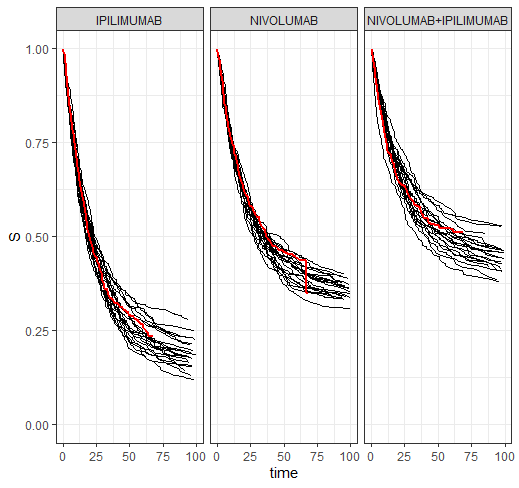
\includegraphics[width=0.4\linewidth, height=5cm]{post_pred_KM_exp_exp_os.png} }}%
    \qquad
    \subfloat[\centering PFS data]{{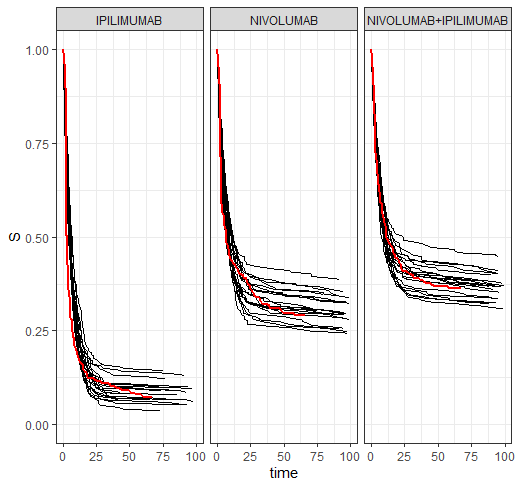
\includegraphics[width=0.4\linewidth, height=5cm]{post_pred_KM_exp_exp_pfs.png} }}%
    \caption{Posterior predictive values Kaplan-Meier curves for exponential OS and exponential PFS distributions with the hierarchical model. Black lines represent outcomes for 20 predicted cohorts and the red line is for the observed data.}%
%     \label{fig:ppv_km_exp}%
% \end{figure}

% \begin{figure}[H]
    \centering
    \subfloat[\centering OS data]{{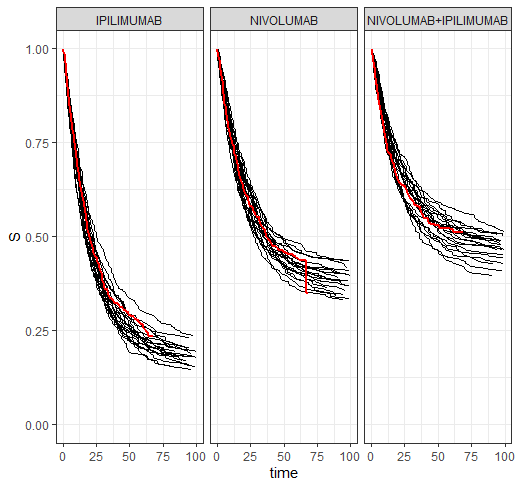
\includegraphics[width=0.4\linewidth, height=5cm]{post_pred_KM_weibull_weibull_os.png} }}%
    \qquad
    \subfloat[\centering PFS data]{{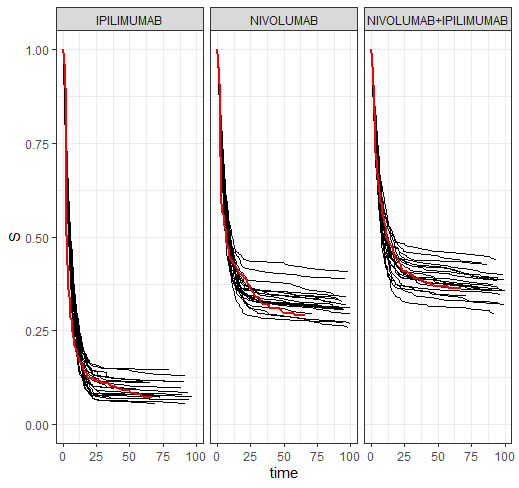
\includegraphics[width=0.4\linewidth, height=5cm]{post_pred_KM_weibull_weibull_pfs.png} }}%
    \caption{Posterior predictive values Kaplan-Meier curves for weibull OS and weibull PFS distributions with the hierarchical model. Black lines represent outcomes for 20 predicted cohorts and the red line is for the observed data.}%
%     \label{fig:ppc_km_wei}%
% \end{figure}

% \begin{figure}[H]
    \centering
    \subfloat[\centering OS data]{{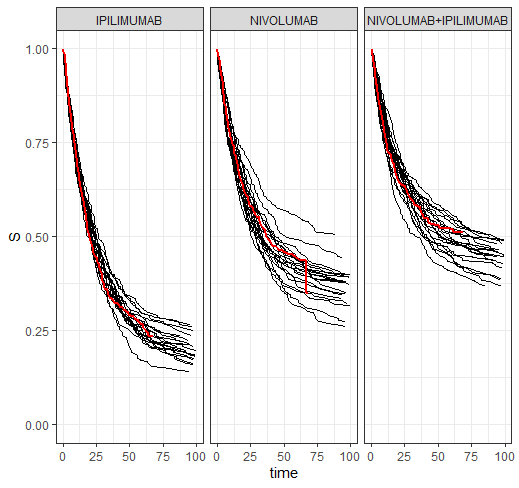
\includegraphics[width=0.4\linewidth, height=5cm]{post_pred_KM_gompertz_gompertz_os.png} }}%
    \qquad
    \subfloat[\centering PFS data]{{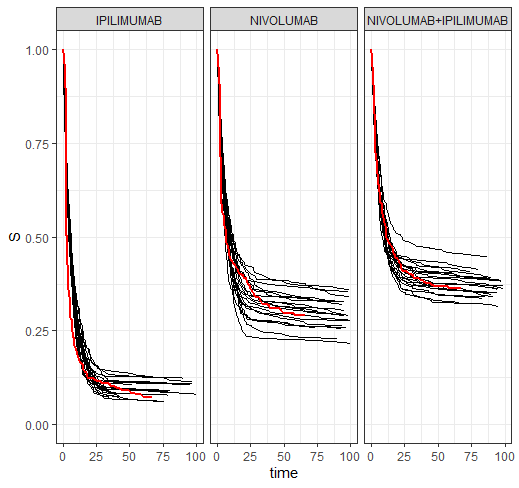
\includegraphics[width=0.4\linewidth, height=5cm]{post_pred_KM_gompertz_gompertz_pfs.png} }}%
    \caption{Posterior predictive values Kaplan-Meier curves for gompertz OS and gompertz PFS distributions with the hierarchical model. Black lines represent outcomes for 20 predicted cohorts and the red line is for the observed data.}%
    % \label{fig:ppv_km_gomp}%
\end{figure}

\newpage

% Stan?
% \begin{lstlisting}[caption = {Descriptive Caption Text}, label=DescriptiveLabel]
% for i:=maxint to 0 do
% \end{lstlisting}

% %\nocite{*}% Show all bib entries - both cited and uncited; comment this line for only cited entries
\bibliography{bibliography}

% \clearpage

% \section*{Author Biography}

% \begin{biography}{
\includegraphics[width=66pt,height=86pt,draft]{empty}}{\textbf{Author Name.} This is sample author is sample author biography text.}
% \end{biography}

\end{document}
